\documentclass{article}

% preamble
  \usepackage[a4paper, top=1in, bottom=1in, left=1in, right=1in]{geometry}
  \usepackage[utf8]{inputenc}
  \usepackage[english]{babel}

  \usepackage{tikz-cd, lipsum, bm, dcolumn}
  \usetikzlibrary{arrows}
  \usepackage{amsmath, amssymb, amsthm, mathrsfs, mathtools, centernot, hyperref, fancyhdr, lastpage}
  \usepackage{extarrows, esvect, esint, pgfplots}
  \pgfplotsset{compat=1.18}

  \setlength{\parindent}{0pt} % set no indent
  \hfuzz=5.0pt % ignore overfull hbox badness warnings below this limit

  \renewcommand{\thispagestyle}[1]{}

  \DeclareMathOperator{\Tr}{Tr}
  \DeclareMathOperator{\Sym}{Sym}
  \DeclareMathOperator{\Span}{span}
  \DeclareMathOperator{\im}{Im}
  \DeclareMathOperator{\Div}{div}
  \DeclareMathOperator{\curl}{curl}
  \DeclareMathOperator{\GL}{GL}
  \DeclareMathOperator{\SL}{SL}
  \DeclareMathOperator{\GA}{GA}
  \DeclareMathOperator{\std}{std}
  \DeclareMathOperator{\Cov}{Cov}
  \DeclareMathOperator{\Var}{Var}
  \DeclareMathOperator{\Corr}{Corr}
  \DeclareMathOperator{\Int}{Int}
  \DeclareMathOperator{\Id}{Id}
  \DeclareMathOperator{\Lie}{Lie}
  \DeclareMathOperator{\Hom}{Hom}
  \DeclareMathOperator{\Alt}{Alt}
  \DeclareMathOperator{\rank}{rank}
  \DeclareMathOperator{\conv}{conv}
  \DeclareMathOperator{\aff}{aff}
  \DeclareMathOperator{\arccot}{arccot}


  \newtheorem{theorem}{Theorem}[section]
  \newtheorem{proposition}[theorem]{Proposition}
  \newtheorem{lemma}[theorem]{Lemma}
  \newtheorem{example}{Example}[section]
  \newtheorem{corollary}{Corollary}[theorem]
  \theoremstyle{remark}
  \newtheorem*{remark}{Remark}
  \theoremstyle{definition}
  \newtheorem{definition}{Definition}[section]
  \renewcommand{\qed}{\hfill$\blacksquare$}
  \renewcommand{\footrulewidth}{0.4pt}% default is 0pt

\begin{document}
\pagestyle{fancy}

\lhead{Ordinary Differential Equations}
\chead{Muchang Bahng}
\rhead{\date{August 2021}}
\cfoot{\thepage / \pageref{LastPage}}

\title{Ordinary Differential Equations}
\author{Muchang Bahng}

\maketitle
\tableofcontents
\pagebreak 

\section{Systems}

  The theory of ordinary differential equations allows us to study all evolutionary processes satisfying three properties. 
  \begin{enumerate}
    \item Deterministic; that is, the entire past and future is determined by its present state. 
    \item Finite-dimensionality; that is, the number of parameters needed to describe any state is finite. 
    \item Differentiability; that is, the phase space of has the structure of a differentiable manifold. 
  \end{enumerate}
  The motion of a system in classical mechanics can be described using ordinary differential equations. However, quantum mechanics, impact theory, fluid mechanics, and heat transfer do not satisfy all three properties. 

  \subsection{Phase Spaces, Phase Flows}

    \begin{definition}
      Given a system that can be represented by a finite number of $1$-dimensional parameters $x_1, x_2, ..., x_n$, each in their respective spaces $X_1, X_2, ..., X_n$, respectively, the \textit{phase space} of the system is the set
      \[S \equiv \prod_{i=1}^n X_i\]
      Notice that each element $s \in S$ represents one specific state of the system. While obvious, it should explicitly be stated that 
      \[\dim{S} = n\]
    \end{definition}

    The abstract notion of a phase space is extremely useful, since we can now model states of the system as points in $S$. As stated before, we can form a general theory and treat $S$ as a differentiable manifold, but for simplicity, we will treat $S = \mathbb{R}^n$. 

    The motion of the entire system can be described by the motion of a point over a curve in the phase space. Since the system is deterministic, the entire motion over this curve is determined by the point itself. 
    \begin{definition}
    Therefore, we can assign a velocity vector at each point $s \in S$ that models the motion of the point, called the \textit{phase velocity vector}. The set of all phase velocity vectors in $S$ is called the \textit{phase velocity vector field} in the phase space $S$. This vector field defines the differential equation of the process. 
    \begin{center}
      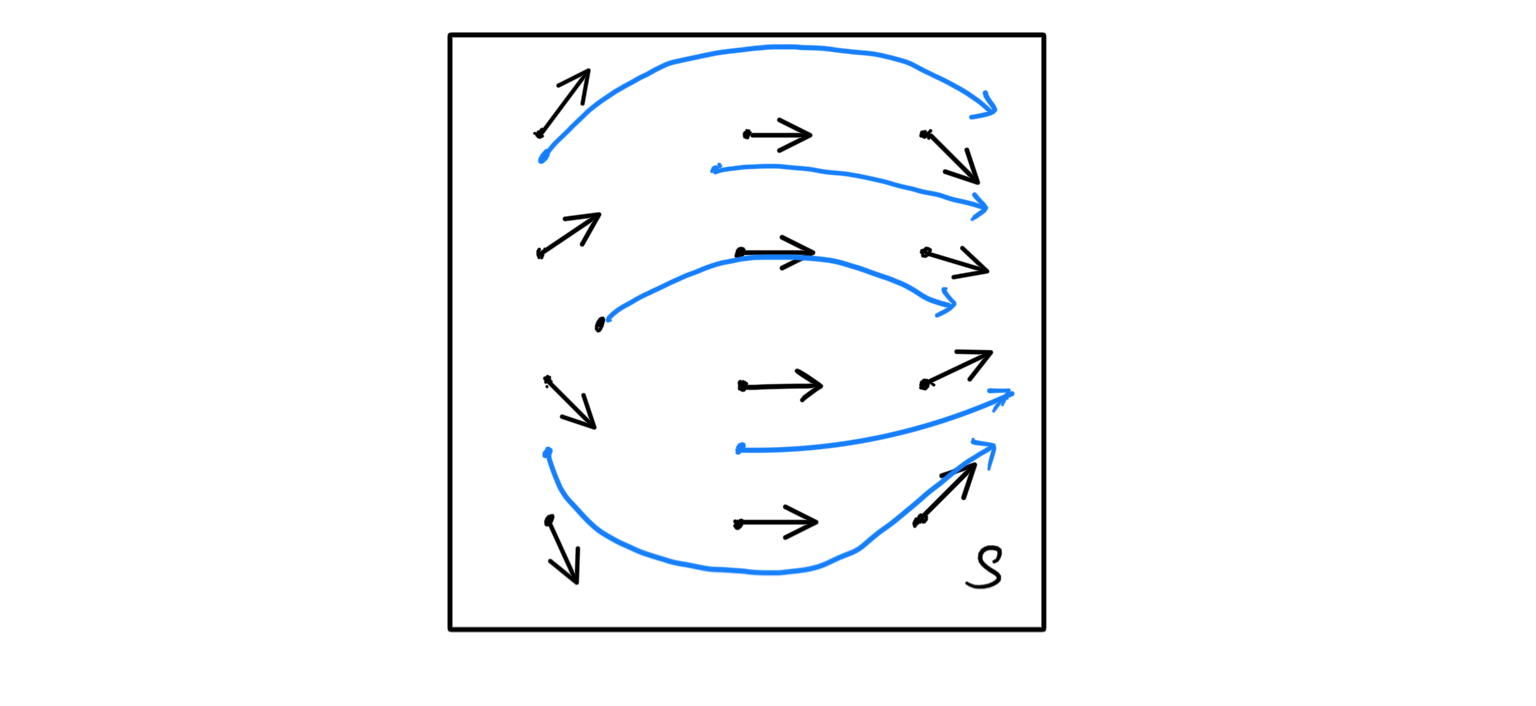
\includegraphics[scale=0.25]{img/Phase_Velocity_Vector_Field.PNG}
    \end{center}
    Since we are trying to model the motion of a point through $S$, it is often convenient to paramaterize the motion as a curve with the time parameter $t$. This creates a well-defined curve (blue curves in the figure above) in a new space that now has a time-axis. 
    \end{definition}


    \begin{definition}
      Given a phase space $S$, the \textit{extended phase space} of a system is the space 
      \[S \oplus \mathbb{R}\]
      where $\mathbb{R}$ represents the new time axis, with parameter $t$. Note that within this theory, negative values of $t$ are well-defined, and $\dim{(S \oplus \mathbb{R})} = n+1$. 
      \begin{center}
        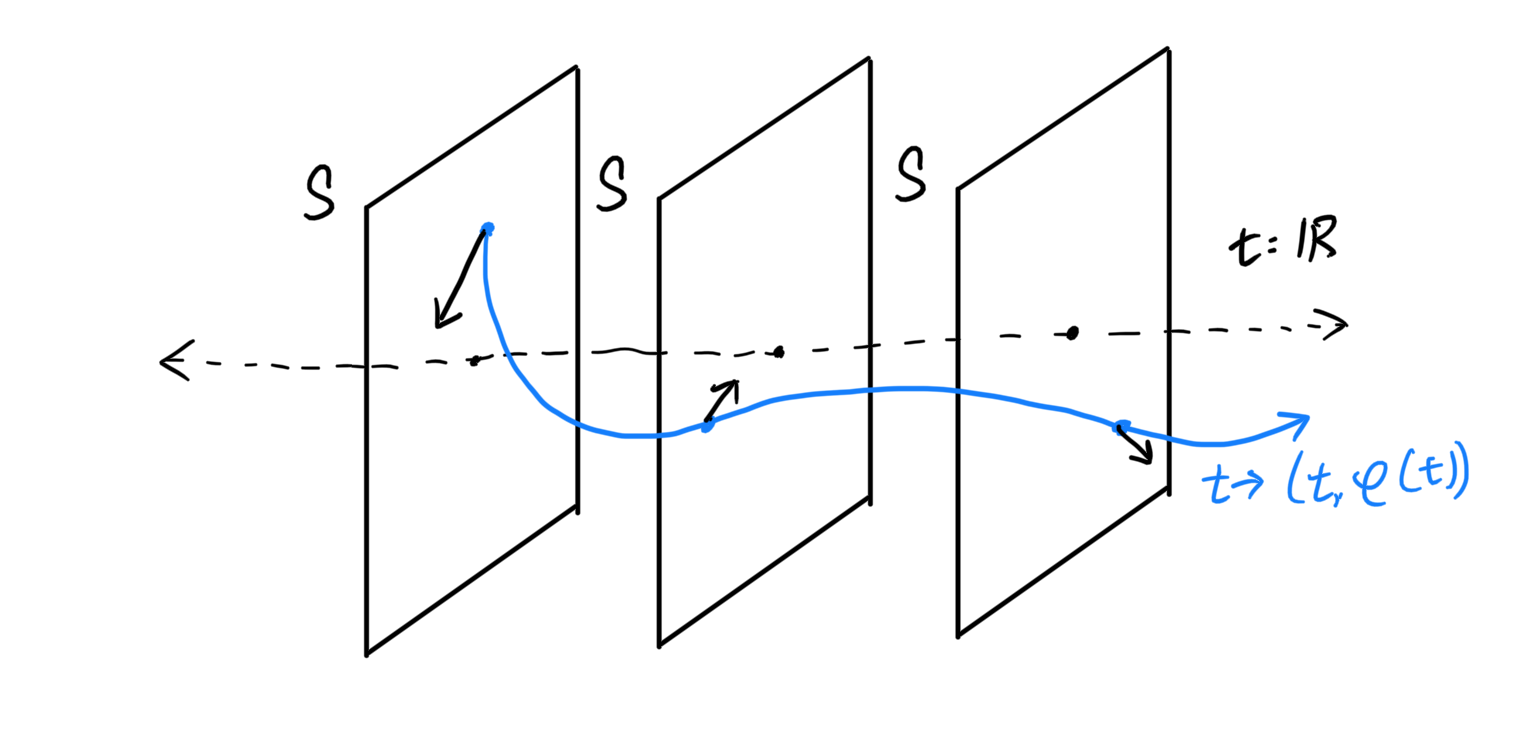
\includegraphics[scale=0.25]{img/Extended_Phase_Space.PNG}
      \end{center}
      The parameterized curve, called the \textit{integral curve}, is defined with the mapping
      \[t \mapsto \big( t, \varphi(t) \big)\]
      where $\varphi$ is the path of the particle through $S$. 
    \end{definition}

    But rather than focusing on the integral curve itself, it is useful to visualize the entire phase velocity field continuously (since we've assumed differentiability) "morphing" with respect to time. This represents a change in the entire system as time passes by. 
    \begin{center}
    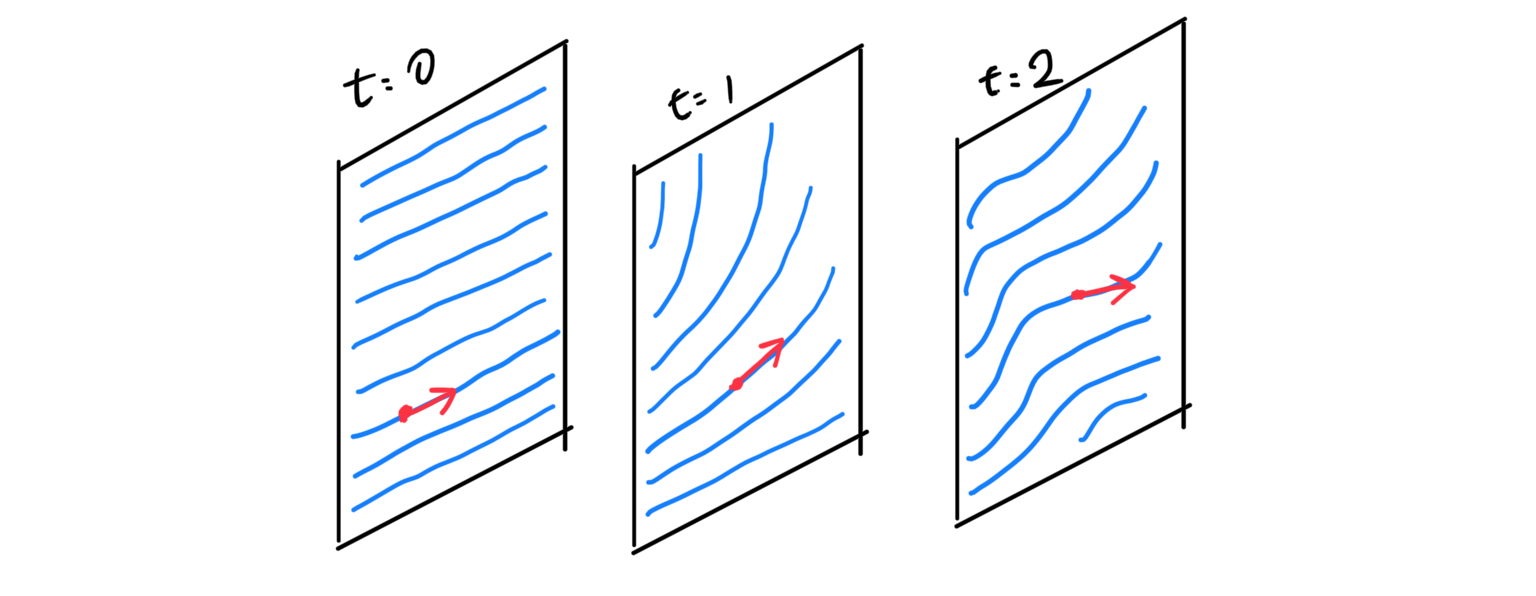
\includegraphics[scale=0.25]{img/Morphing_Field.PNG}
    \end{center}
    With this visual in mind, we can see that there may be multiple integral curves that can go through $S \oplus \mathbb{R}$. To determine a unique integral curve, it may be necessary to define an \textit{initial point} that represents an initial condition. 

    However, there may be some systems that are invariant under time. For example, swinging a pendulum or the movement of a particle is only dependent on the position and velocity of the pendulum and particle. Whether we let go of the pendulum at $t=0$ or $t=1$ does not matter. This is what we call an \textit{autonomous} system. 

    \begin{definition}
    An \textit{autonomous}, or \textit{time-homogeneous}, system is a system where the phase space does not have a time parameter. We can visualize this type of system as one where the phase velocity vector does not morph at all. 
    \begin{center}
        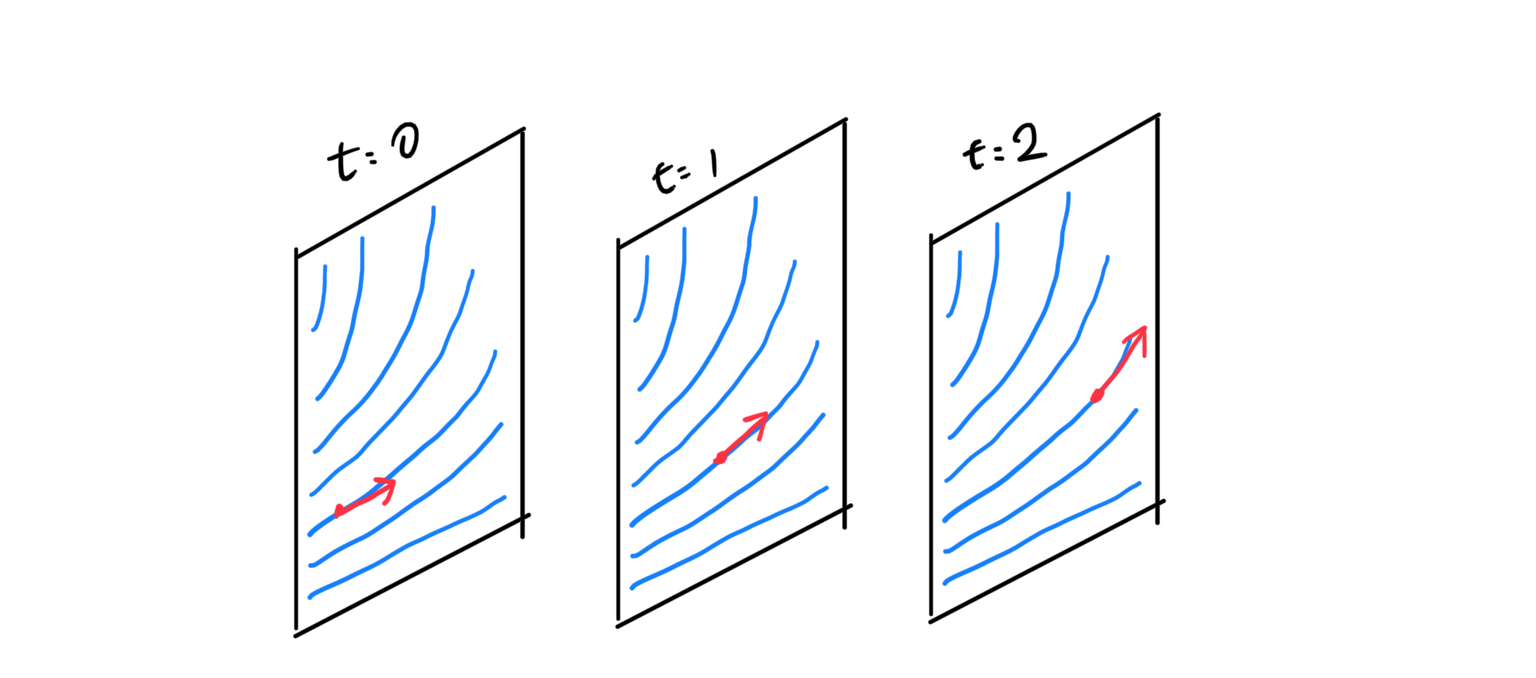
\includegraphics[scale=0.25]{img/Autonomous_Field.PNG}
    \end{center}
    \end{definition}

    \begin{example}[1-Dimensional Autonomous System]
    Another special type of system is one that produces a one dimensional \textit{constant} phase field that changes in the same way everywhere with respect to time. We can visualize it as a vector field in $\mathbb{R}$ that stays constant as time passes (left). Since it may be hard to visualize vectors in $\mathbb{R}$, we can view them as slopes. 
    \begin{center}
        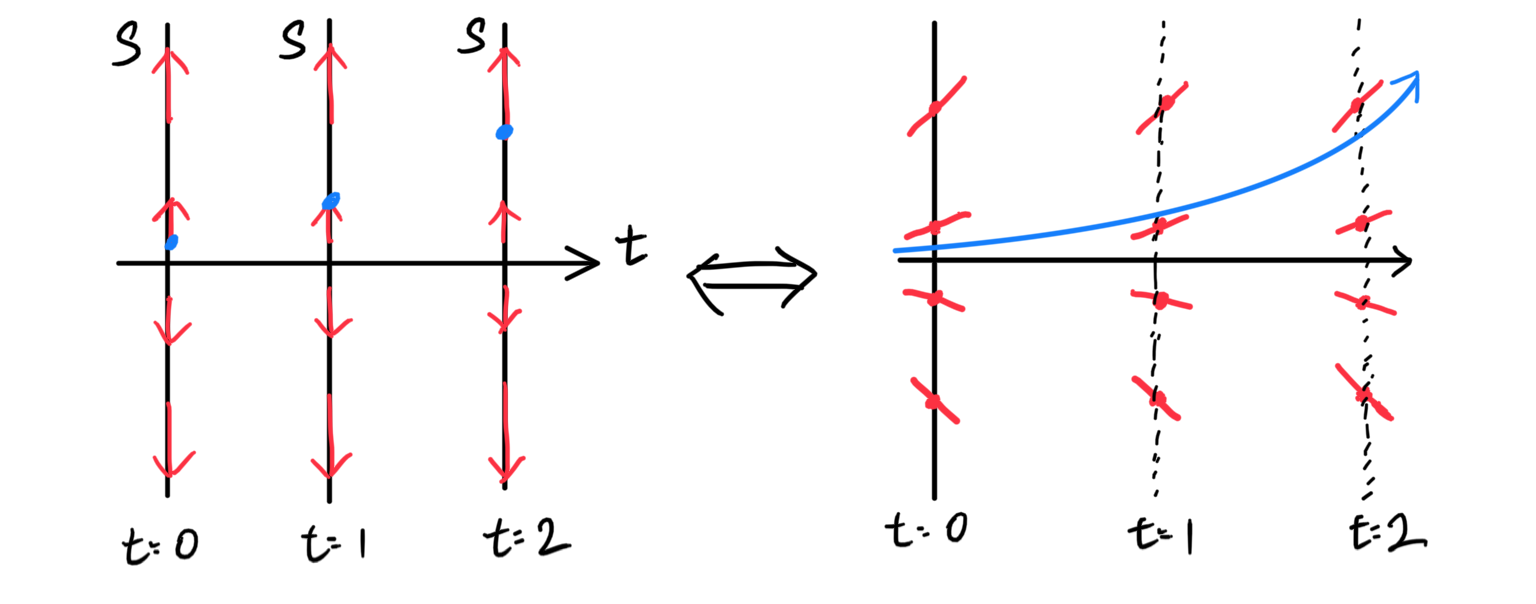
\includegraphics[scale=0.25]{img/One_dim_auto_system.PNG}
    \end{center}
    \end{example}

    \begin{example}[1-Dimensional General System]
    A one dimensional system can be visualized as the initial vector field of $\mathbb{R}$ at $t=0$ gradually morphing as time passes. 
    \begin{center}
        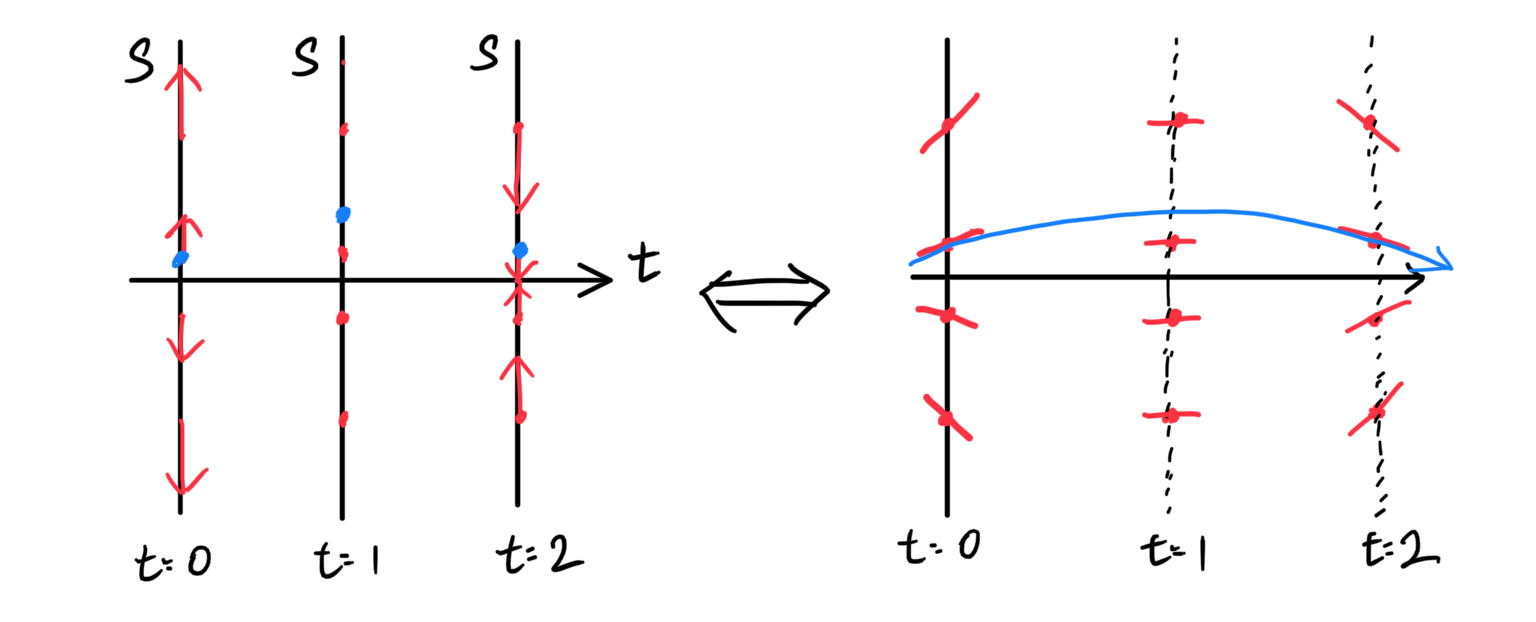
\includegraphics[scale=0.25]{img/One_dim_general_system.PNG}
    \end{center}
    \end{example}

    \begin{example}[1-Dimensional Non-Autonomous Constant System]
    Let $\nu$ be a constant, one-dimensional non-autonomous phase velocity field that changes with respect to time $t$. 
    \begin{center}
        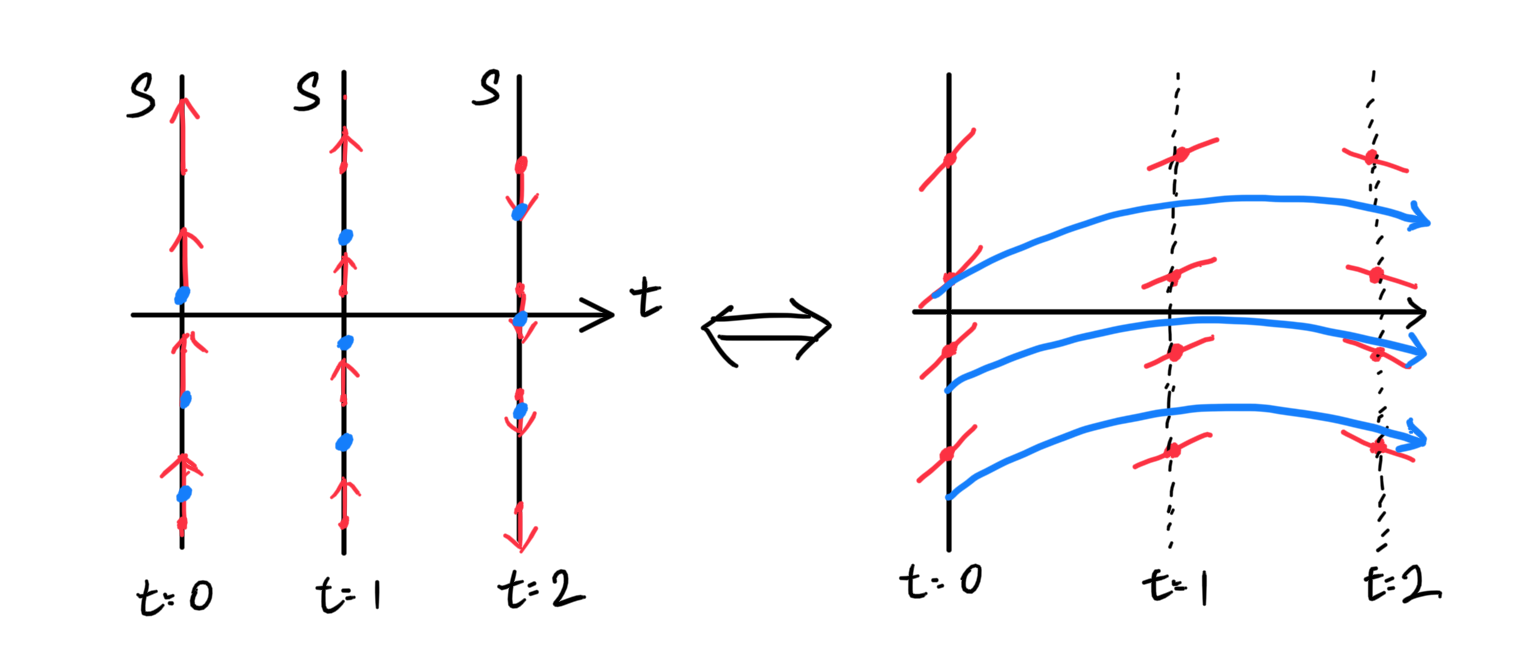
\includegraphics[scale=0.25]{img/Nonauto_constant_field.PNG}
    \end{center}
    Then, the function $\varphi$ in which its graph $\big( t, \varphi(t)\big)$ precisely overlaps the integral curves of $\nu$ can be computed by \textit{Barrow's formula}
    \[\varphi(t) = x_0 + \int_{t_0}^t \nu(\tau)\, d\tau\]
    Where $(t_0, x_0)$ is the initial condition of the system, and $\tau$ is a dummy variable representing time. 
    \end{example}

    It is also worthwhile to note that we can define the function to exist within a certain subset of the phase space and to be defined over a certain time interval within $\mathbb{R}$, rather than requiring it to be defined on the whole space itself. We will denote the time interval $I \subset \mathbb{R}$ and the subset $U \subset S$. 
    \begin{center}
        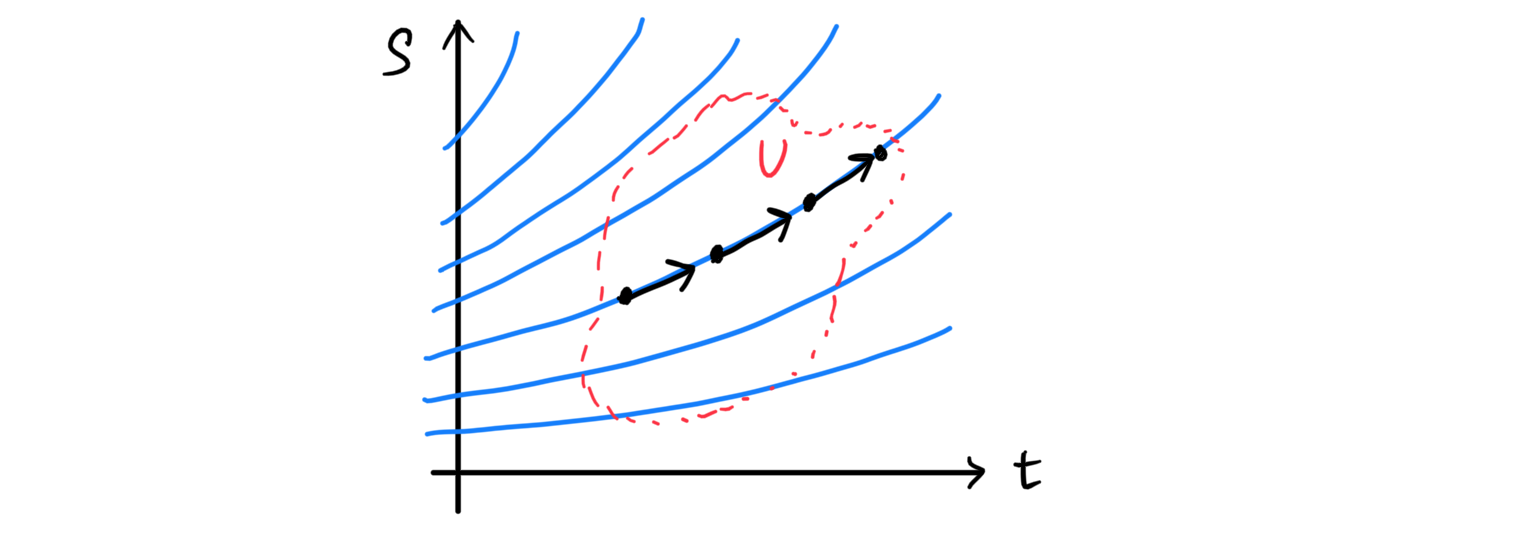
\includegraphics[scale=0.25]{img/ODE_in_open_set.PNG}
    \end{center}

    \subsubsection{Dimensionality vs Order}

      \begin{definition}[Dimensionality of a System]
      The \textit{dimensionality} of the phase space of a system is dependent upon many things: 
      \begin{enumerate}
          \item the dimension of the space that we are working in
          \item the number of particles or bodies that we observe
          \item other factors, like orientation, that may add extra parameters 
      \end{enumerate}
      But colloquially, the more things we have to keep track in the system, the higher the dimensionality. 
      \end{definition}

      \begin{definition}[Order of a System]
      Formally, the \textit{order} of a differential equation is the highest order derivative that is contained within the equation. It has nothing to do with how many moving parts there are (i.e. dimensionality) and more with the rule that each moving part follows. 
      \end{definition}


      \begin{example}
      We will state a couple examples of how many dimensions certain systems would have: 
      \begin{enumerate}
          \item A point particle moving in three dimensional space in a constant force field would have $3$ spatial dimensions (each represented by a second order differential equation). Note that a constant force field means that acceleration is also constant, so acceleration is not taken into account. 
          \begin{center}
              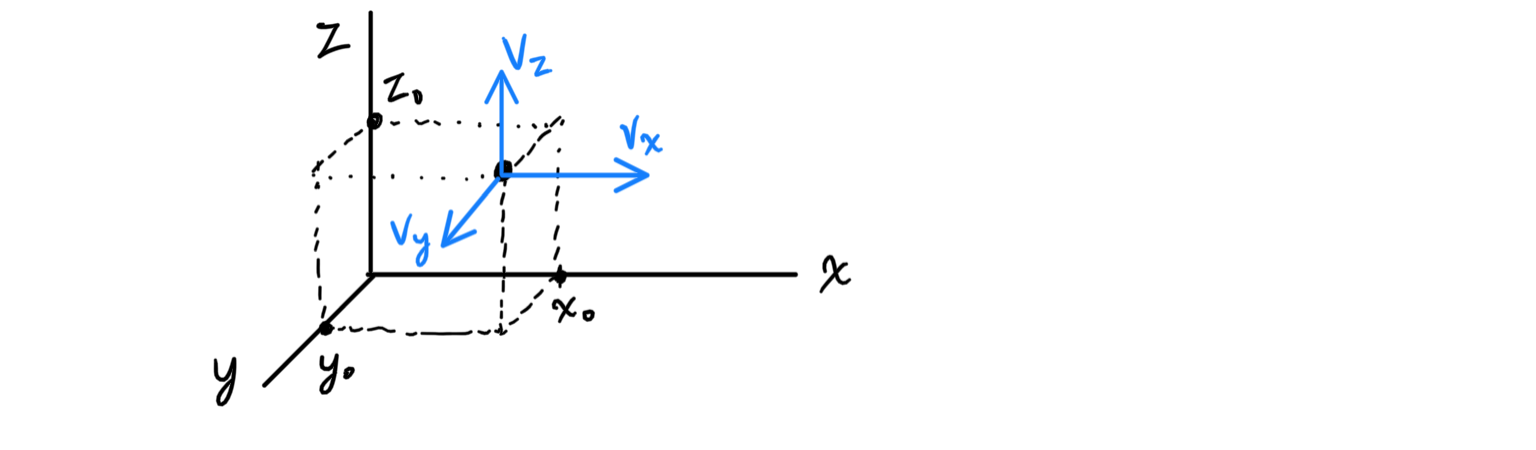
\includegraphics[scale=0.25]{img/Point_Moving_in_Space.PNG}
          \end{center}
          \item A rigid body in 3-space has 6 parameters (3 for its center of mass and 3 for its orientation). 
          \begin{center}
              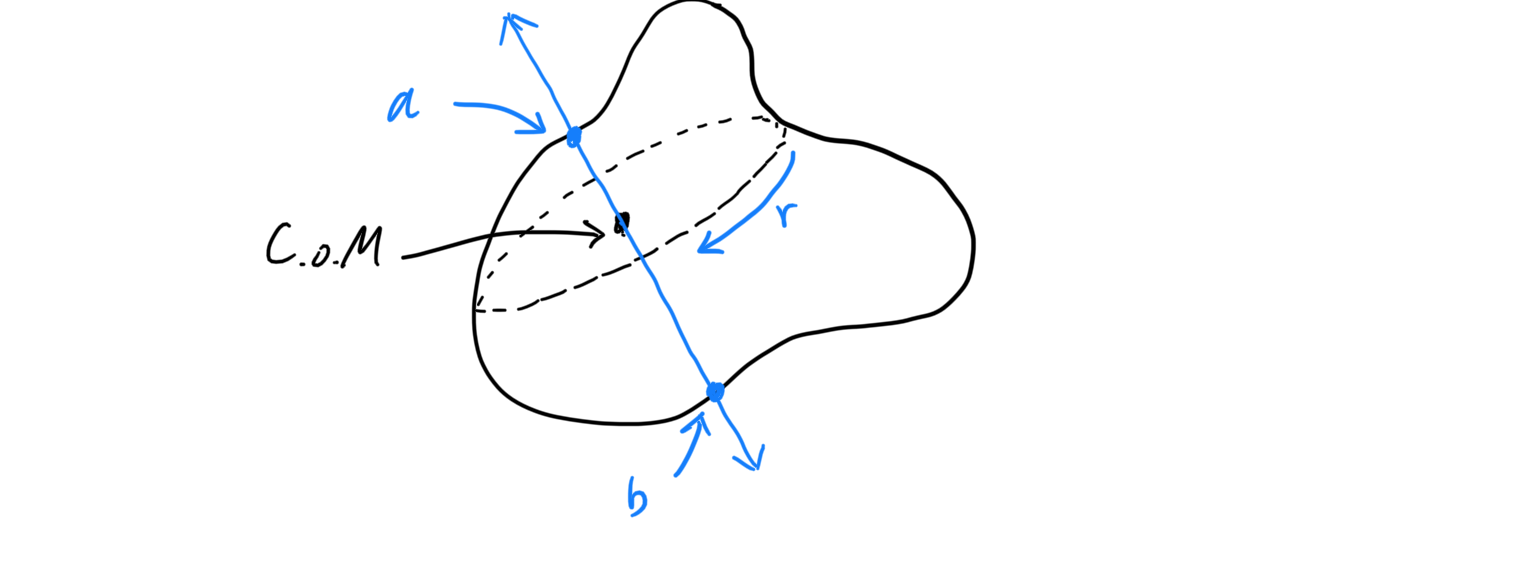
\includegraphics[scale=0.25]{img/Rigid_Body.PNG}
          \end{center}
          Therefore, a system of 3 rigid bodies in 3-space has a total of $6 \times 3 = 18$ dimensions, where each body is individually following $F = ma$ where the force $F$ is given by the gravitational force. This gives a second order differential equation for each body in terms of the positions of the other bodies. 
          \begin{center}
              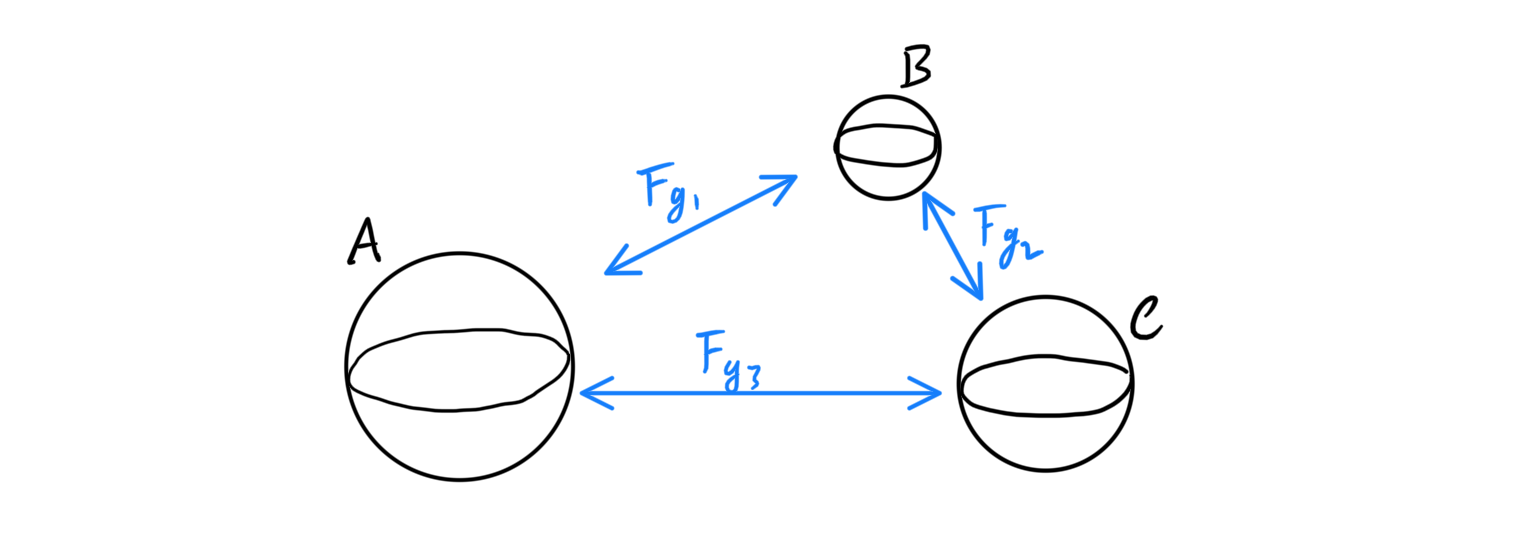
\includegraphics[scale=0.25]{img/System_of_3_Rigid_Bodies.PNG}
          \end{center}
      \end{enumerate}
      \end{example}

  \subsection{First Order Differential Equations}

    The simplest types of differential equations are systems that contain parameters displacement and first derivative (velocity). Note that this does not necessarily mean that the dimension of the phase space is $1$. 

    \begin{definition}[n-dimensional First Order Differential Equation]
    An \textit{n-dimensional first order differential equation} is an equation of the form
    \[y^\prime = f(t, y)\]
    where $y$ is an $n$-dimensional vector representing the displacement parameters of the system, $t$ is the time parameter, and
    \[f(t_0, \cdot) : \mathbb{R}^n \longrightarrow \mathbb{R}^n\]
    is an $n$-dimensional vector field that determines the phase velocity field of $S$ at time $t = t_0$. It can also be written explicitly as a system as 
    \[\begin{pmatrix}
    y_1^\prime \\ y_2^\prime \\ \vdots \\ y_n^\prime
    \end{pmatrix} = \begin{pmatrix}
    f_1 (t, y) \\ f_2 (t, y) \\ \vdots \\ f_n (t, y)
    \end{pmatrix}\]
    This equation defines an $n$-dimensional phase velocity field that morphs as time passes, which is used to model the movement of the $n$-dimensional system. Simply put, the velocity vector that determines the evolution of the system is completely dependent on the current state of the system (value of $y$) and the time (value of $t$). 

    The solution to this system is a smooth map $\varphi: I \subset \mathbb{R} \longrightarrow U \subset \mathbb{R}^n$ defined by the integral curve $t \mapsto (t, \varphi(t))$ in the extended phase space that satisfies the equation
    \[\varphi^\prime (t) = f\big( t, \varphi(t) \big)\]
    \end{definition}

    \subsubsection{Basic One-Dimensional Examples}

      \begin{example}[Normal Reproduction]
      Assume that the size of a biological population is $y$ and that the rate of reproduction is proportional to the number of organisms present. This is expressed by the first order differential equation of dimension 1 
      \[y^\prime = k y, \;\; k > 0\] 
      \begin{center}
          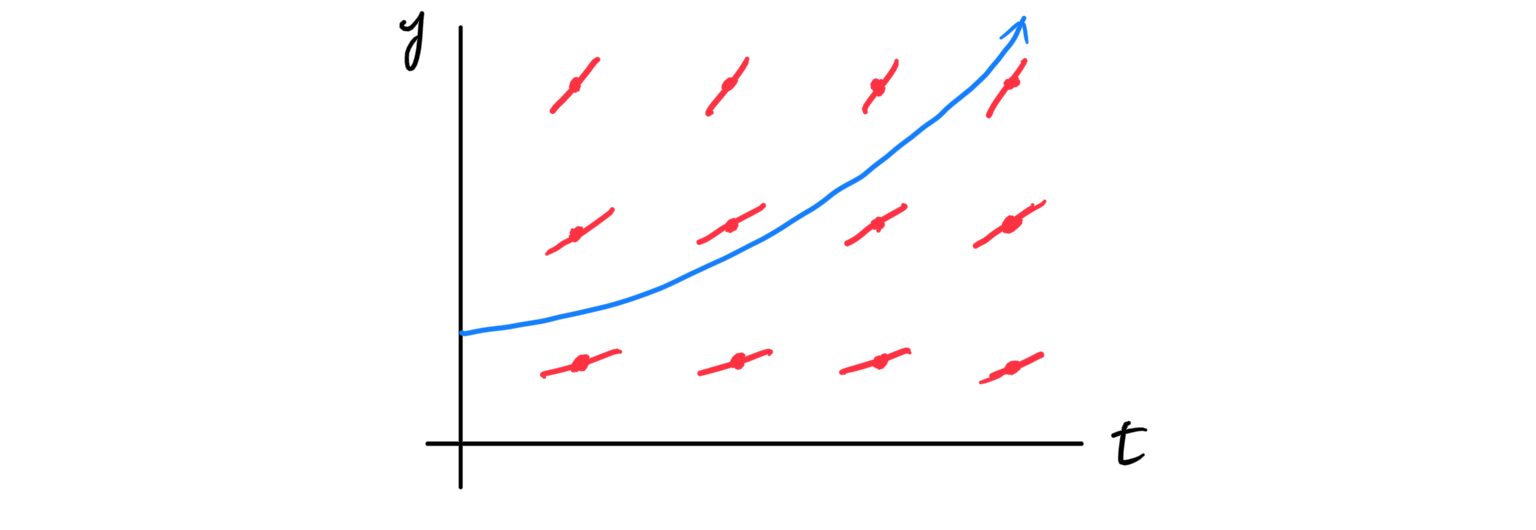
\includegraphics[scale=0.2]{img/Normal_Reproduction.PNG}
      \end{center}
      The solution to the equation, given initial conditions $(t_0, y_0)$ is 
      \[\varphi(t) = e^{k (t - t_0)} y_0\]
      \end{example}

      \begin{example}[Explosion Equation]
      If we assume that the rate of reproduction is proportional to the number of pairs of individuals, we get the differential equation 
      \[y^\prime = k y^2\]
      The integral curves of this equation shoot off to infinity in a finite time, while the integral curves of the normal reproduction system reaches infinite when $t$ is infinite. 
      \begin{center}
          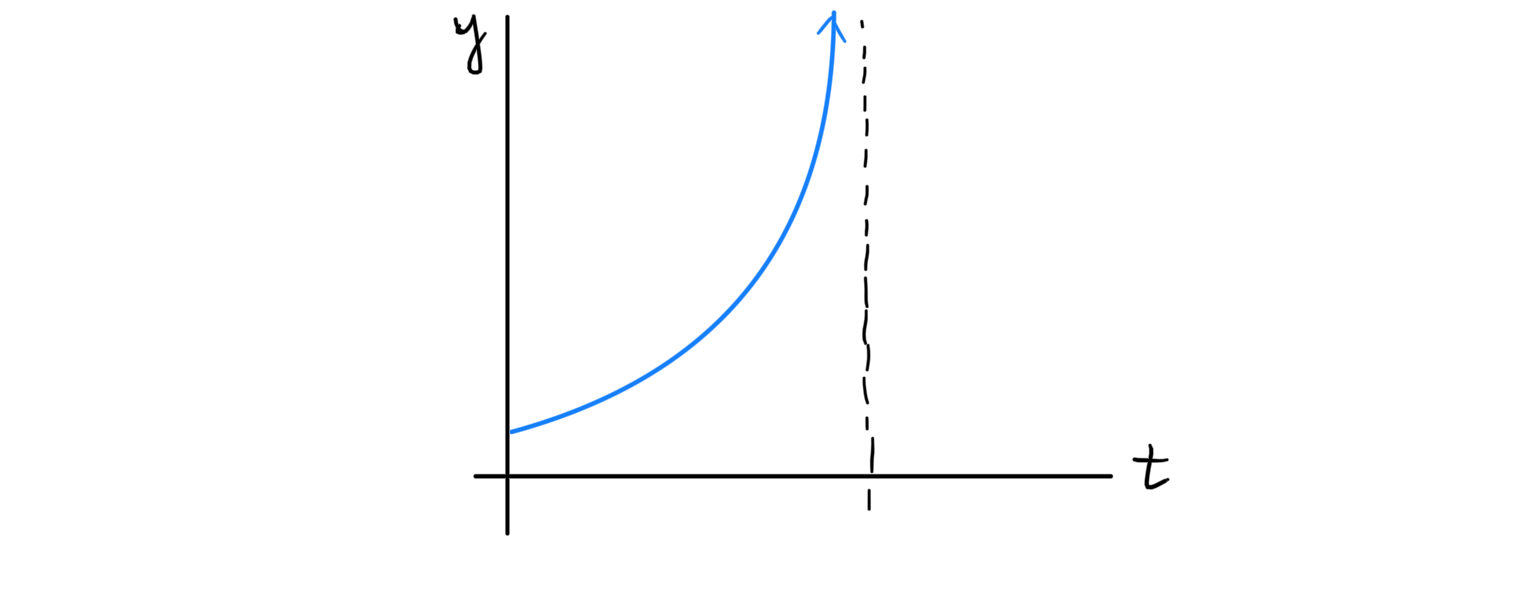
\includegraphics[scale=0.25]{img/Explosion_Equation.PNG}
      \end{center}
      \end{example}

      \begin{example}[Logistic Curve]
      Due to limiting factors that may restrict the rate of growth of a population, we modify the equation to the following \textit{logistic equation}. 
      \[x^\prime = (1 - x) x\]
      Both the direction field and the integral curves are shown. 
      \begin{center}
          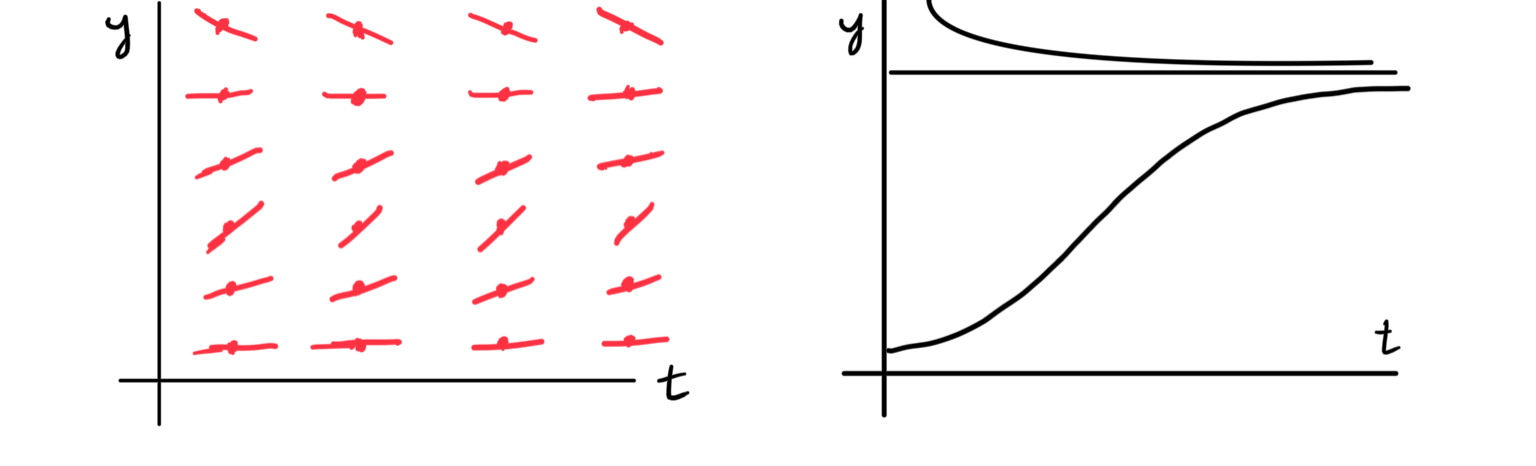
\includegraphics[scale=0.15]{img/Logistic_Curve.PNG}
      \end{center}
      \end{example}

      \begin{example}[Harvest Quotas]
      Now, we model a situation where we harvest a part of the population. Let us first assume that the rate of harvest is constant. This leads to the differential equation
      \[x^\prime = (1 - x) x - c\]
      The quantity $c$ represents the rate of harvesting and is called the \textit{quota}. For different values of $c$, this results in the integral curves. 
      \begin{center}
          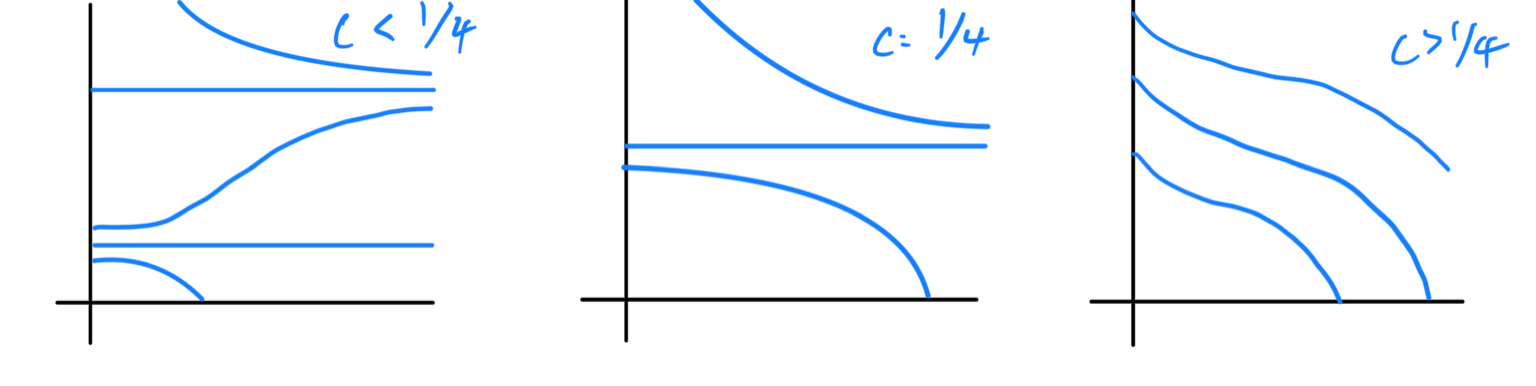
\includegraphics[scale=0.2]{img/Harvest_Quotas.PNG}
      \end{center}
      However, if we harvest with a relative quota, represented by the equation
      \[x^\prime = (1 - x) x - p x\]
      for $0 < p < 1$, this leads us to an integral curve with a stable equilibrium point. 
      \begin{center}
          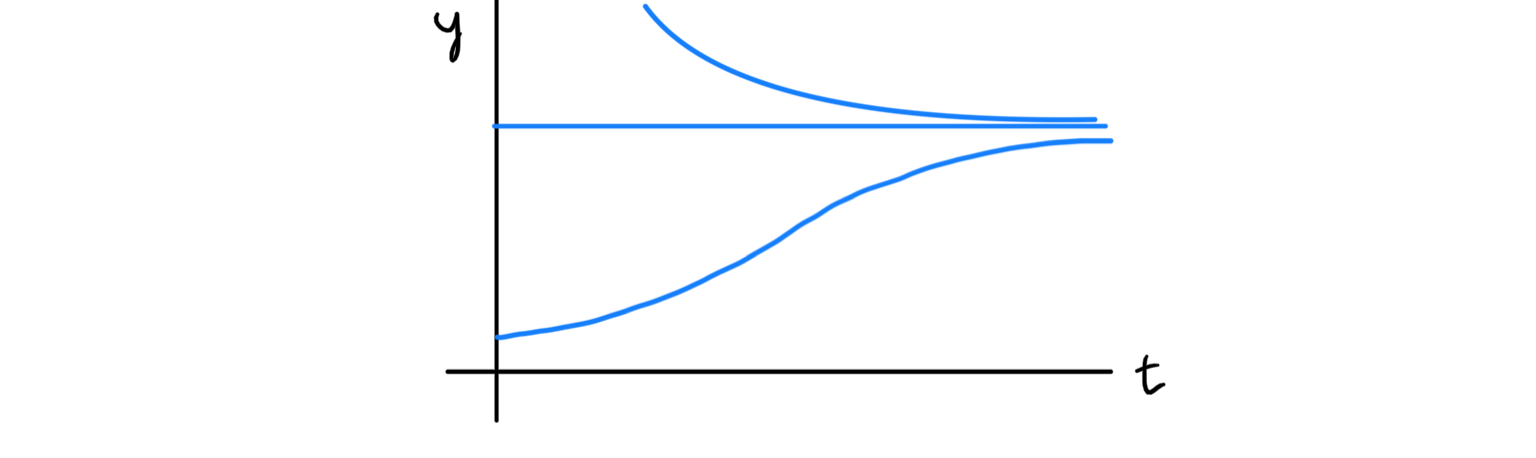
\includegraphics[scale=0.2]{img/Relative_Quota.PNG}
      \end{center}
      \end{example}

    \subsubsection{Additional Examples}

      \begin{example}[Lotka-Volterra Model]
      The simplest model describing the predator-prey relationship between two species is described by the system of differential equations (also a $2$-dimensional first order differential equation). 
      \begin{align*}
          & x^\prime = k x - a x y \\
          & y^\prime = - l y + b x y
      \end{align*} 
      The phase space with its velocity vector field can be defined by defining the vector 
      \[\begin{pmatrix}
      kx - axy \\ -ly + bxy
      \end{pmatrix}\]
      at each point in $\mathbb{R}^2$, labeled with the $x$ and $y$ axes. 
      \begin{center}
          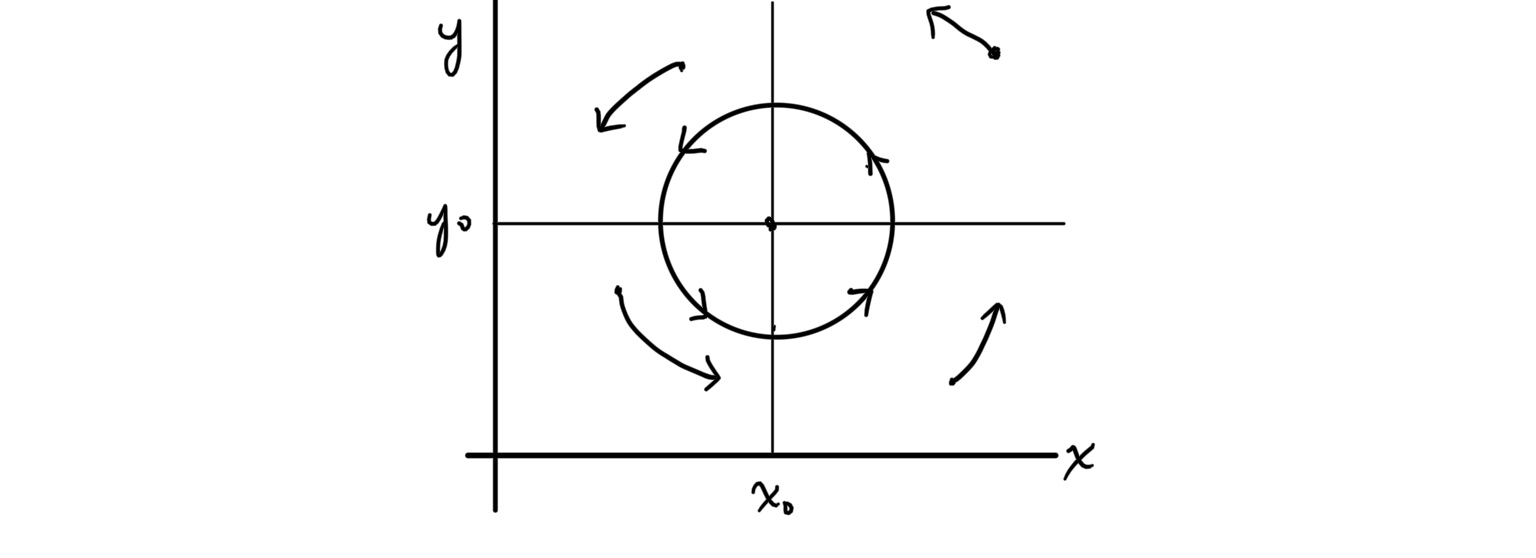
\includegraphics[scale=0.25]{img/Lotka_Volterra.PNG}
      \end{center}
      Note that we have graphed the model such that the two parameters $x, y$ are shown and not the time, but note that the time parameter $t$ very much exists in this autonomous model. 
      \begin{center}
          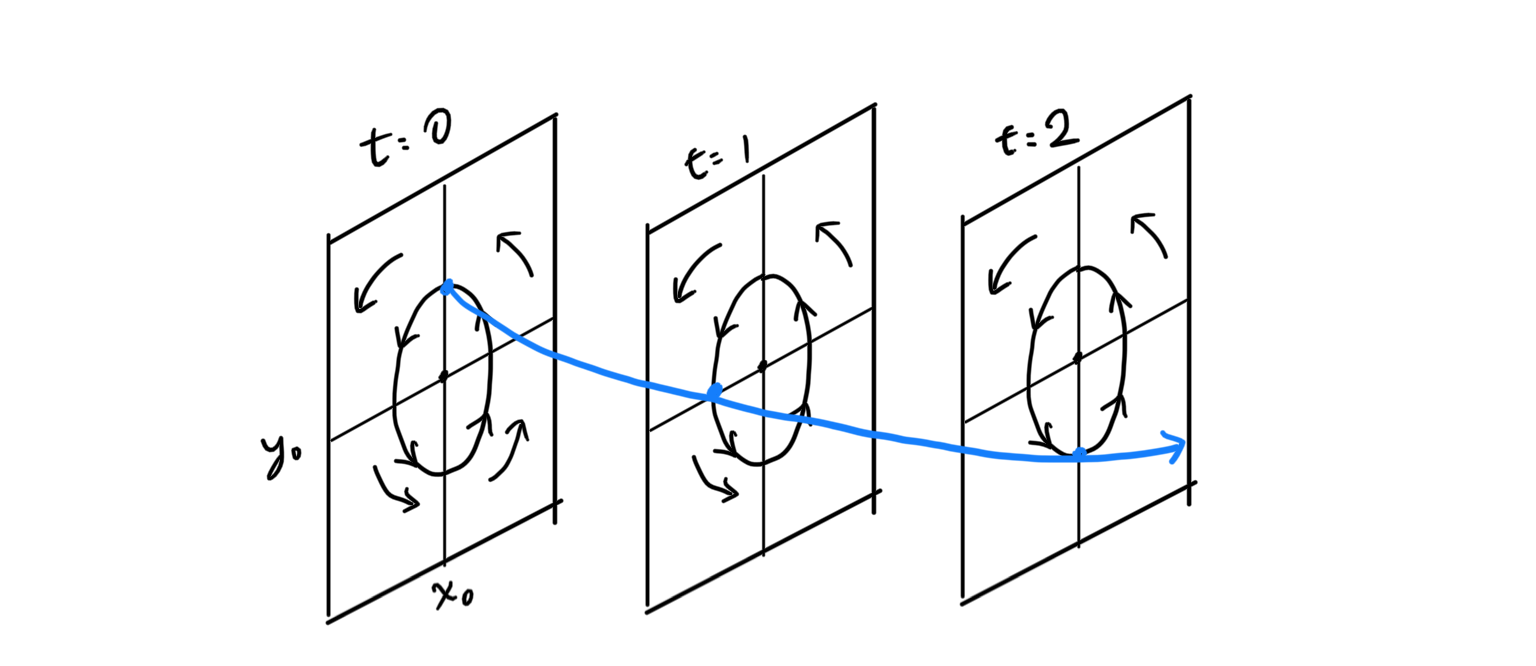
\includegraphics[scale=0.25]{img/Lotka_Autonomous.PNG}
      \end{center}
      The blue curve is the solution to this system, which describes the evolution of the autonomous system as time passes. 
      \end{example}

      \begin{example}[Pendulums]
      Small oscillations of a pendulum can be approximated, using Taylor approximations, to get the differential equation 
      \[x^{\prime \prime} = - k x\]
      By scaling the coefficient $k$, we can make it equal to $1$ to get
      \[x^{\prime \prime} = -x\]
      The phase space of this system is 2 dimensional, with parameters $x_1 = x$ and $x_2 = x^\prime$. This creates the autonomous system of first order differential equations
      \[x^\prime_1 = x_2, \; x_2^\prime = -x_1\]
      This leads to the phase velocity vector field shown below. 
      \begin{center}
          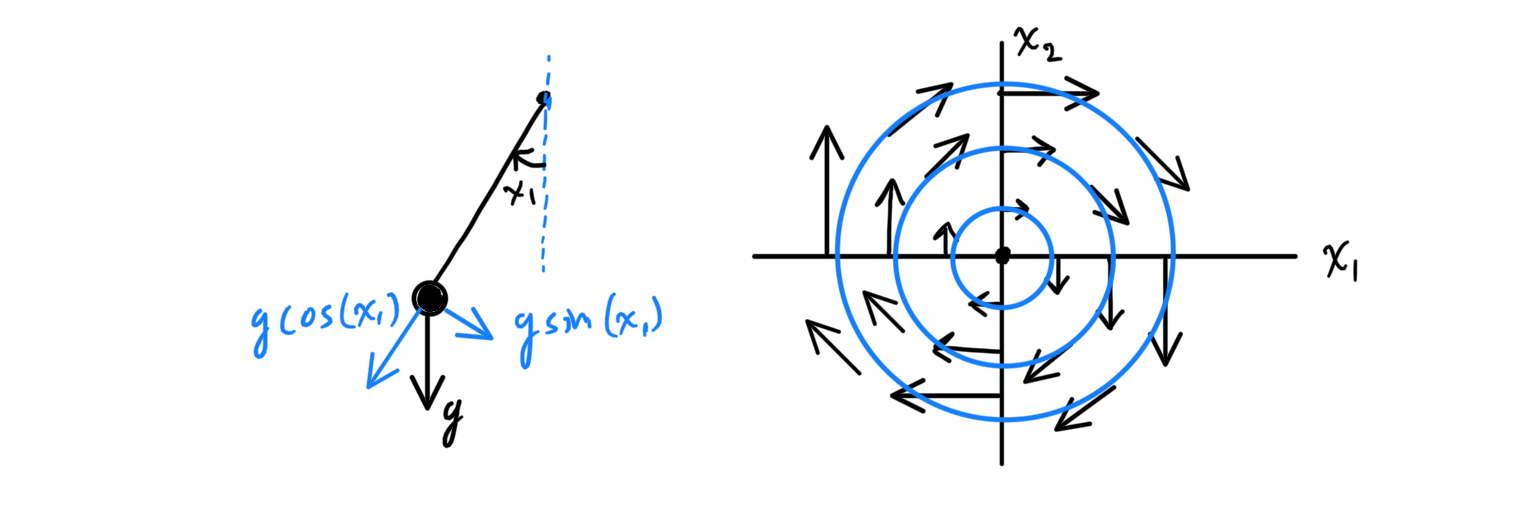
\includegraphics[scale=0.25]{img/Undampened_Simple_Pendulum.PNG}
      \end{center}
      A more accurate equation for the undampened pendulum system (by scaling $k$ again) is 
      \[\theta^{\prime \prime} = -\sin{\theta}\]
      Clearly, the solution to this system, given initial value of $(x_1^*, x_2^*)$, is a helix.
      \begin{center}
          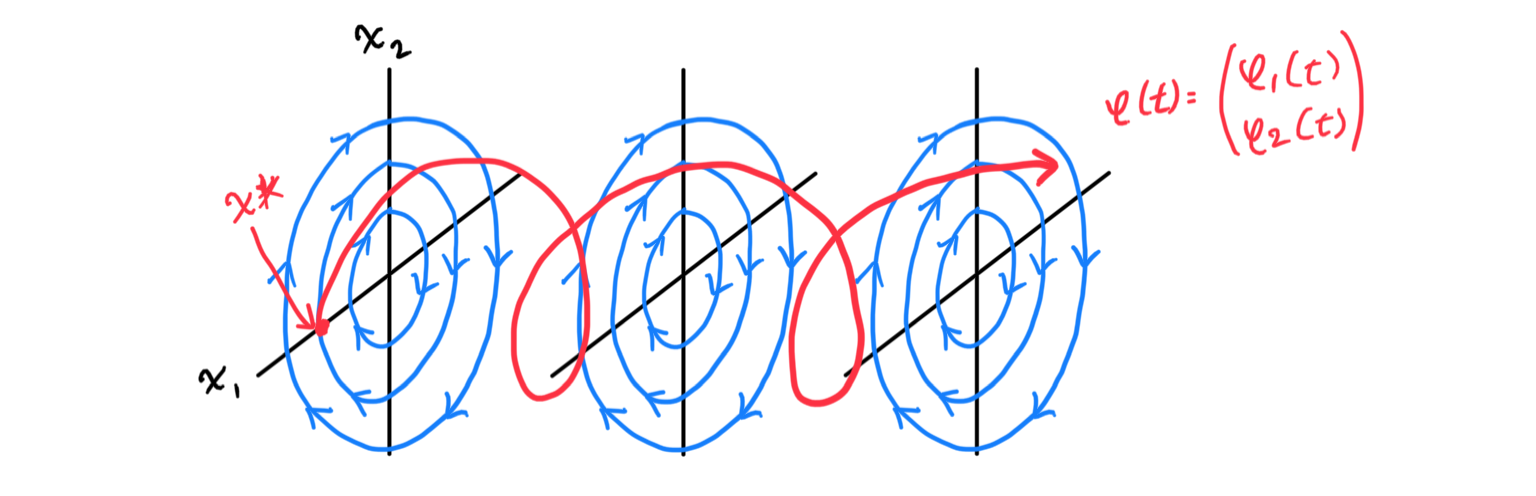
\includegraphics[scale=0.25]{img/Helix_Solution.PNG}
      \end{center}
      This equation can be represented as the autonomous system
      \[x_1^\prime = x_2, \; x_2^\prime = - \sin{x_1} \]
      which creates the phase velocity vector field
      \begin{center}
          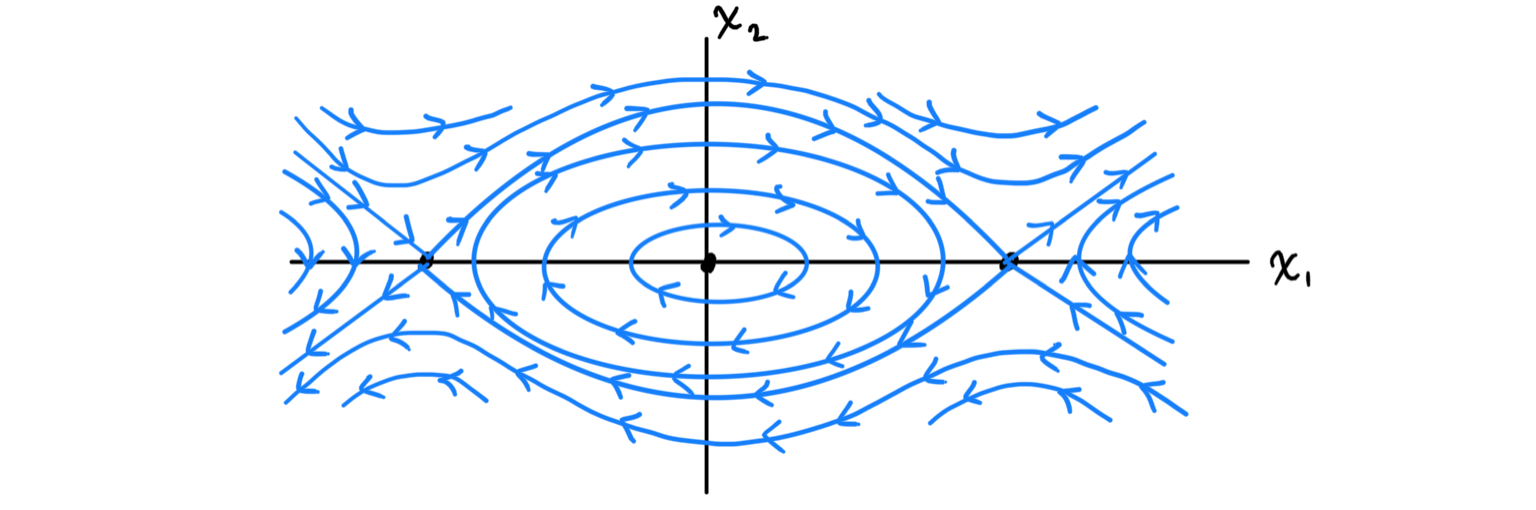
\includegraphics[scale=0.25]{img/Undampened_Accurate_Pendulum.PNG}
      \end{center}
      \end{example}

      \begin{example}[Small Oscillations of Spherical Pendulums]
      A spherical pendulum adds another dimension of movement (another dimension of angle and angular velocity), therefore inducing a system where the phase space is 4 dimensional. For small oscillations, the differential equations
      \[x^{\prime\prime} = -x, \; y^{\prime\prime} = - y\]
      is represented with the system
      \[x_1^\prime = x_2, \; x_2^\prime = -x_1, \; x_3^\prime = x_4, \; x_4^\prime = - x_3\]
      where $x_1 = x, x_2 = x^\prime, x_3 = y, x_4 = y^\prime$. 
      \end{example}

  \subsection{Existence Theory}

    Before we introduce methods to solve differential equations, we will state and prove conditions for existence and uniqueness of solutions. We will only prove existence in the simplest case. 
    \begin{theorem}[Existence of Solutions in a First-Order System with Phase Space Dimensionality of 1]
    Let $f$ and $\partial f / \partial y$ be $C^0$ functions in a given region $U \in \mathbb{R}^2$, with $(t_0, y_0) \in D$. This means that 

    Then, there exists an interval $I$ containing $t_0$ and exactly $1$ solution $\varphi$ of the differential equation 
    \[y^\prime = f(t, y)\]
    passing through $(t_0, y_0)$. The solution exists for values of $t$ for all points $\big(t, \varphi(t)\big) \in U$. $\varphi$ is also a continuous function with respect to $(t, t_0, y_0)$. 
    \end{theorem}
    In order to state the proof, we will introduce some lemmas. 

    \begin{lemma}
    $\varphi$ is a solution to $y^\prime = f(t, y)$ with $\varphi(t_0) = y_0$ on interval $I$ if and only if $\varphi$ satisfies the solution $y$ of the equation
    \begin{equation}
        y(t) = y_0 + \int_{t_0}^t f\big( s, y(s)\big) \,ds, \;\; t \in I
    \end{equation}
    \end{lemma}
    \begin{proof}
    $(\rightarrow)$ $\varphi$ is a solution of $y^\prime = f(t, y)$, with $\varphi(t_0) = y_0 \implies \varphi^\prime (t) = f \big(t, \varphi(t) \big)$
    \begin{align*}
        \implies & \int_{t_0}^t \varphi^\prime (s) \,ds = \int_{t_0}^t f \big( s, \varphi(s) \big) \, ds \\
        \implies & \varphi(t) = \varphi(t_0) + \int_{t_0}^t f\big(s, \varphi(s)\big) \,ds = y_0 + \int_{t_0}^t f \big( s, \varphi(s) \big) \,ds
    \end{align*}
    $(\leftarrow)$ $y(t)$ is a solution of (1) $\implies y(t)$ is continuous by the fundamental theorem of calculus. Since $f$ is also continuous, $y(t)$ is differentiable. 
    \[\implies y^\prime (t) = \frac{d}{dt} \bigg( y_0 + \int_{t_0}^t f\big( s, y(s) \big) \, ds \bigg) = f\big(t, y(t) \big)\]
    Putting $t=t_0, y (t_0) = y_0$, this implies that $y$ is a solution of $\varphi^\prime (t) = f(t, y)$. 
    \end{proof}

    The previous lemma allows us to establish the existence of a solution using (1), which is generally easier. We now define the Lipshitz inequality for functions of two variables. 

    \begin{definition}
    Let $f(t, y)$ be a continuous, bounded function in region $D$. For all $(t, y_1), (t, y_2) \in D$, if $f$ satisfies the inequality 
    \[|f(t, y_2) - f(t, y_1)| \leq K |y_2 - y_1|\]
    then $f$ is said to satisfy the \textit{Lipshitz condition} in $D$.
    \end{definition}

    Now, we define a series of successive approximations
    \[\varphi_0 (t) = y_0, \; \varphi_{j+1} (t) = y_0 + \int_{t_0}^t f\big(s, \varphi_j (s) \big) \, ds\]
    We hope that this sequence will eventually converge onto the actual $\varphi$, but we must propertly define the $\varphi_j$'s such that the points remain in the region $D$. 

    \begin{lemma}
    Let $\alpha = \min\{a, \frac{b}{M}\}$. Then, the successive approximations $\varphi_j$ are defined on the interval $I$ given by $|t - t_0| < \alpha$, and on this interval 
    \begin{equation}
        |\varphi_j (t) - y_0| \leq M |t - t_0| < b, \;\; j = 0, 1, 2, ...
    \end{equation}
    \end{lemma}
    \begin{proof}
    Clearly, $\varphi_0 (t)$ is defined on $I$ and satisfies (2). Now assuming that for $n \geq 1$, $\varphi_n$ is defined and satisfies (2) $\implies$ the point $\big( t, \varphi(t)\big) \in D$ for $t \in I$. To prove that $\big(t, \varphi_{n+1}(t)\big) \in D$, we already know $t \in I$, so we must show that $|\varphi_{n+1} (t) - y_0| < b$. Using the intermediate value theorem,
    \begin{align*}
        |\varphi_{n+1}(t) - y_0| & = \bigg| \int_{t_0}^t f\big(s, \varphi_j(s)\big) \, ds \bigg| \\
        & \leq \bigg| \int_{t_0}^t |f\big(s, \varphi_j (s)\big)|\, ds\bigg| \\
        & \leq M |t - t_0| < M\alpha < \leq b
    \end{align*}
    We specifically assign $\alpha$ because first, (2) implies that the successive approximations also have slopes bounded by the cone of the lines with slope $M$ and $-M$ through points $(t_0, y_0)$. The length $\alpha$ of $I$ depends on where these lines meet $D$. Either way, the $\varphi_j$'s remain in the rectangles.
    \end{proof}

    Now, we can prove an existence theorem. 

    \begin{theorem}
    Suppose $f$ and $\partial f/\partial y$ are continuous and bounded on the rectangle $D$ satisfying the Lipshitz condition. That is, 
    \[|f(t, y)| \leq M, \;\; \Big| \frac{\partial f}{\partial y} \Big| \leq K\]
    Then, the sucessive approximations $\varphi_j$ (defined previously) converge uniformly on the interval $I = (t_0 - \alpha, t_0 + \alpha)$ to a solution $\varphi$ of the differential equation $y^\prime = f(t, y)$ with $\varphi(t_0) = y_0$. 
    \end{theorem}
    \begin{proof}
    The second lemma shows that $\varphi_j$ are defined on the interval $I$. Now, we define the difference between $\varphi_j$ adn $\varphi_{j+1}$ in the interval $[t_0, t_0 + \alpha]$ and $[t_0 - \alpha, t_0]$. Using the Lipshitz condition, 
    \begin{align*}
        r_j (t) = |\varphi_{j+1} (t) - \varphi_j (t)| & = \bigg| \int_{t_0}^t f\big(s, \varphi_j (s)\big) - f\big(s, \varphi_{j-1} (s) \big) \,ds\bigg| \\
        & \leq \int_{t_0}^t |f\big(s, \varphi_j (s)\big) - f\big( s, \varphi_{j-1} (s)\big)|\,ds \\
        & \leq K \int_{t_0}^t \varphi_j (s) - \varphi_{j-1} (s) \,ds \\
        & = K \int_{t_0}^t r_{j-1} (s) \,ds, \;\; j = 1, 2, ...
    \end{align*}
    When $j=0$, 
    \begin{align*}
        r_0 (t) = |\varphi_1 (t) - \varphi_0 (t)| & = \bigg| \int_{t_0}^t f \big(s, \varphi(s)\big) \,ds \bigg| \\
        & \leq \int_{t_0}^t |f\big(s, \varphi(s)\big)\,ds \leq M (t - t_0) 
    \end{align*}
    Now, using induction, we prove that 
    \[r_j (t) \leq \frac{M K^j (t-t_0)^{j+1}}{(j+1)!}, \;\; j = 0, 1, 2, ...; t_0 \leq t \leq t_0 + \alpha\]
    The base case suffices. When $j=0$, 
    \[r_0 (t) \leq M (t-t_0)\]
    Now assume that the statement is true for $j=p-1$, for $p \geq 1$. Then, 
    \begin{align*}
        r_p (t) \leq K \int_{t_0}^t r_{p-1} (s) \, ds & \leq K \int_{t_0}^t \frac{M K^{p-1} (s - t_0)^p}{p!} \,ds \\
        & = \frac{M K^p}{p!} \cdot \bigg( \frac{(s-t_0)^{p+1}}{p+1} \bigg|_{t_0}^t \bigg) \\
        & = \frac{M K^p (s - t_0)^{p+1}}{(p+1)!}, \;\; t_0 \leq t \leq t_0 + \alpha
    \end{align*}
    \end{proof}
    Integrating this fact into the main proof, we have
    \begin{align*}
        r_j (t) \leq \frac{M K^j |t - t_0|^{j+1}}{(j+1)!} & = \frac{M (K |t - t_0|)^{j+1}}{K (j+1)!}\\
        & < \frac{M \alpha^{j+1} K^{j+1}}{K (j+1)!} \\
        & = \frac{M (K \alpha)^{j+1}}{K (j+1)!} 
    \end{align*}
    This implies that
    \begin{align*}
        \sum_{j=0}^\infty r_j (t) & = \frac{M}{K} \sum_{j=0}^\infty \frac{ (K \alpha)^{j+1}}{(j+1)!} \\
        & = \frac{M}{K} e^{\alpha K} \\
    \end{align*}
    This implies that 
    \[\sum_{j=0}^\infty \big( \varphi_{j+1} (t) - \varphi_{j} (t) \big)\]
    absolutely and uniformly converges in the interval $I$ where $|t - t_0| < \alpha$ to some function of $t$, determined arbitrarily by $\varphi (t)$. 

    To see the rate and error bound of convergence, we already defined
    \begin{align*}
        & \varphi(t) = \varphi_0 (t) + \sum_{n=0}^\infty \big(\varphi_{n+1} (t) - \varphi_n (t)\big) \\
        \implies & \varphi (t) - \varphi_j (t) = \sum_{n=0}^\infty \big(\varphi_{n+1} (t) - \varphi_n (t)\big) \\
        \implies & |\varphi(t) - \varphi_j (t)| \leq \sum_{n=j}^\infty |\varphi_{n+1} (t) - \varphi_n (t)| \\
        & \leq \sum_{n=j}^\infty r_n (t) \leq \frac{M}{K} \sum_{n=j}^\infty \frac{(K \alpha)^{n+1}}{(n+1)!} \\
        & \leq \frac{M}{K} \frac{(K \alpha)^{j+1}}{(j+1)!} \sum_{n=0}^\infty \frac{(K\alpha)^n}{n!} = \frac{M}{K} \frac{(K\alpha)^{j+1}}{(j+1)} e^{K \alpha}
    \end{align*}
    It is clear that 
    \[\epsilon_j = \frac{(K \alpha)^{j+1}}{(j+1)!} \rightarrow 0 \text{ as } j \rightarrow \infty\]
    To prove continuity of $\varphi(t)$ on $I$, we let $\epsilon > 0$ and assign 
    \begin{align*}
        \varphi(t+h) - \varphi(t) & = \varphi(t+h) - \varphi_j (t+h) + \varphi_j (t+h) - \varphi_j (t) + \varphi_j (t) - \varphi(t) 
    \end{align*}
    which, by the triangle inequality, implies that
    \begin{align*}
        \implies |\varphi(t+h) - \varphi(t)| & \leq |\varphi(t+h) \varphi_j  (t+h)| + |\varphi_j (t+h) - \varphi_j (t)| + |\varphi_j (t) - \varphi(t)| \\
        & \leq 2 \varepsilon_j + |\varphi_j (t+h) - \varphi_j (t)| 
    \end{align*}
    Choosing $j$ sufficiently large and $|h|$ sufficiently small, using 
    \[\lim_{j \rightarrow \infty} \varepsilon_j = 0\]
    and continuity of $\varphi_j (t)$, we can make
    \[|\varphi(t+h) - \varphi(t)| \leq |\varphi_j (t+h) - \varphi_j (t)| < \varepsilon, \;\; \text{as } h \rightarrow 0\]
    $\implies \varphi(t)$ is continuous since the limit exists at $t$ that matches the actual value. 

    To show that the $\varphi(t)$ satisfies the integral equation in the first lemma, we see that
    \begin{align*}
        \lim_{j \rightarrow \infty} \varphi_j (t) = \varphi(t) & \implies \lim_{j \rightarrow \infty} \int_{t_0}^t f\big( s, \varphi_j (s)\big) \, ds = \int_{t_0}^t f\big(s, \varphi(s)\big) \,ds \\
        & \implies \lim_{j \rightarrow \infty} \varphi_{j+1} (t) = \lim_{j \rightarrow \infty} \bigg( y_0 \int_{t_0}^t f \big(s, \varphi_j (s)\big) \,ds\bigg) \\
        & \implies \varphi (t) = y_0 + \int_{t_0}^t f\big(s, \varphi_ (s) \big) \, ds 
    \end{align*}
    Using the first lemma, we see that $\varphi$ therefore satisfies the differential equation $y^\prime = f(t, y)$ with initial conditions $\varphi(t_0) = y_0$. 

    \begin{corollary}
    The error committed by $\varphi_j (t)$ satisfies the estimate 
    \[|\varphi (t) - \varphi_j (t)| \leq \frac{M}{K} \frac{(K \alpha)^{j+1}}{(j+1)!} e^{K \alpha} \;\;\; \forall t \in I\]
    In fact, the conditions of this theorem implies the uniqueness of solutions of $y^\prime = f(t, y)$. However, we can prove existence without uniqueness. 
    \end{corollary}

    \begin{theorem}
    Suppose $f \in C^0$ in rectangle $R$ with $f$ bounded; that is, $|f(t, y)| \leq M$ for all $(t, y) \in R$. Let $\alpha = \min\{a, b /M\}$. Then, there exists a solution $\varphi$ of differential equation
    \[y^\prime = f(t, y)\]
    with $\varphi(t_0) = y_0$ existing on interval $|t - t_0| < \alpha$. 
    \end{theorem}

    Now, we prove the uniqueness of solutions. 
    \begin{lemma}[Gronwall Inequality]
    Let $K > 0$ be a constant, and $f, g \in C^0$ be nonnegative on interval $\alpha \leq t \leq \beta$ satisfying 
    \[f(t) \leq K + \int_\alpha^t f(s)\,g(s) \,ds \;\; \forall t \in [\alpha, \beta]\]
    Then, 
    \[f(t) \leq K \exp \bigg( \int_{\alpha}^t g(s) \,ds \bigg) \;\; \forall t \in [\alpha, \beta]\]
    \end{lemma}
    \begin{proof}
    Let 
    \[U(t) = K + \int_\alpha^t f(s) \, g(s) \, ds \implies U (\alpha) = K\]
    Then, $f(t) \leq U(t)$, which implies, by the fundamental theorem of calculus and $g(t) \geq 0$, that 
    \begin{align*}
        & U^\prime (t) = f(t)\,g(t) \leq U(t) \, g(t) \;\; (\alpha \leq t \leq \beta) \\
        \implies & U^\prime (t) - U(t) \, g(t) \leq 0
    \end{align*}
    which implies
    \begin{align*}
        & U^\prime (t) \bigg( - \exp \Big( \int_\alpha^t g(s) \, ds \Big)\bigg) - U(t) \, g(t) \bigg( - \exp \Big( \int_\alpha^t g(s) \, ds \Big)\bigg) \\
        & = \Bigg( U(t) \bigg( - \exp \Big( \int_\alpha^t g(s) \, ds \Big)\bigg) \Bigg)^\prime \leq 0 \\
        \implies & \int_\alpha^t \frac{d}{dr} \bigg( U(r) \bigg( - \exp \Big( \int_\alpha^r g(s) \, ds \Big)\bigg) \bigg) \,dr \\
        & = U(t) \, \exp \Big( -\int_\alpha^t g(s)\,ds \Big) - U(\alpha) \leq 0 \\
        \implies & f(t) \leq U(t) \leq U(\alpha) \, \exp \Big( \int_\alpha^t g(s)\,ds \Big) = K \exp \Big( \int_\alpha^t g(s) \, ds\Big) 
    \end{align*}
    \end{proof}

    \begin{theorem}
    Let $f, \partial f/ \partial y \in C^0$ be bounded in rectangle $R \equiv \{(t, y) \;|\; |t-t_0| < \alpha, |y - y_0| < b\}$. Then there exists at most one solution of $y^\prime = f(t, y)$ satisfying $\varphi(t_0) = y_0$. 
    \end{theorem}
    \begin{proof}
    Since the hypothesis of this theorem establishes the existence of at least one solution $\varphi$, it suffices to prove that any two solutions are equal. Assume that $\varphi_1, \varphi_2$ are two different solutions on a common interval $J$. By the first lemma, we have for all $t \in J$
    \begin{align*}
        &\varphi_1 (t) = y_0 + \int_{t_0}^t f\big(s, \varphi_1 (s)\big) \,ds \\
        &\varphi_2 (t) = y_0 + \int_{t_0}^t f\big(s, \varphi_2 (s)\big) \,ds
    \end{align*}
    which implies (using the Lipshitz condition) that
    \begin{align*}
        & \varphi_2 (t) - \varphi_1 (t) = \int_{t_0}^t f\big(s, \varphi_2 (s)\big) - f\big(s, \varphi_1 (s)\big) \, ds \\
        \implies & |\varphi_2 (t) - \varphi_1 (t)| \leq \bigg|\int_{t_0}^t |f\big(s, \varphi_2 (s)\big) - f\big(s, \varphi_1 (s)\big)| \, ds\bigg| \\
        & \leq K \bigg| \int_{t_0}^t |\varphi_2 (s) - \varphi_1 (s) | \bigg|
    \end{align*}
    Using Gronwall's inequality and setting $K=0, g(s) = 1$, and $f(t) = |\varphi_2 (t) - \varphi_1 (t)|$, we have
    \[\leq K \bigg| \int_{t_0}^t |\varphi_2 (s) - \varphi_1 (s) | \bigg| \leq 0 \cdot \exp \bigg( \int_{\alpha}^t 1\,ds \bigg) = 0\]
    $\implies |\varphi_2 (t) - \varphi_1 (t)| = 0 \implies \varphi_1 = \varphi_2$, a contradiction. 
    \end{proof}

    Finally, we prove continuity of $f$ with respect to initial conditions. 
    \begin{theorem}
    let $f, \partial f/ \partial y \in C^0$ be bounded in region $D$ and satisfy the Lipshitz condition. Let $\varphi$ be the solution of $y^\prime = f(t, y)$ with $\varphi(t_0) = y_0$ and let $\psi$ be the solution of $y^\prime = f(t, y)$ with $\psi(\hat{t}_0) = \hat{y}_0$. Assume that $\varphi$ and $\psi$ both exist on interval $[a, b]$. Then for each $\varepsilon > 0$, there exists a $\delta > 0$ such that if $|t - \hat{t}| < \delta$ and $|y - \hat{y}| < \delta$, then 
    \[|\varphi(t) - \psi(\hat{t})| < \varepsilon, \;\; a < t, \hat{t} < b\]
    \end{theorem}

\section{Methods of Solution}

  \subsection{Basic Methods for First Order Scalar-Valued DEQs}

    \subsubsection{Variables Separable}

      \begin{definition}[Separable DEQs and Solution]
      A differential equation in the form
      \[y^\prime = g(t) h(y)\]
      is called a \textit{variables-separable equation}. 

      Assume that given solution $\varphi$, $h\big( \varphi(t)\big) \neq 0$ for all $t \in I$. Then, we rearrange the equation and integrate either indefinitely or definitely, where $y = \varphi(t)$. Note that there is no difference between finding solutions using indefinite or definite integration. 
      \[\varphi^\prime (t) = g(t) h(\varphi(t)) \implies \frac{y^\prime}{h(y)} = g(t)\]
      \begin{enumerate}
          \item Indefinitely, we can use substitution $y = \varphi(t)$ to get
          \[\int \frac{\varphi^\prime (t)}{h(\varphi(t))} \, dt = \int g (t) \, dt \implies \int \frac{1}{h(y)} \,dy = \int g(t)\,dt\]
          This can be remembered with the mnemonic
          \[\frac{dy}{dt} = g(t) h(y) \implies \frac{1}{h(y)} dy = g(t) dt \implies \int \frac{1}{h(y)} dy = \int g(t) dt\]
          \item Definitely, we can use the same substitution $y = \varphi(s)$, where $y_0 = \varphi(t_0)$, to get
          \[\int_{t_0}^t \frac{\varphi^\prime (s)}{h(\varphi(s))} \, ds = \int_{t_0}^t g(t)\, dt \implies \int_{y_0}^y \frac{1}{h(\Tilde{y})} \, d\Tilde{y} = \int_{t_0}^t g(\Tilde{t})\, d\Tilde{t}\]
          where we can treat $\Tilde{y}$ and $\Tilde{t}$ as dummy variables. 
      \end{enumerate}
      Both methods define the solution implicitly, but it may or may not be possible to solve it explicitly as $y = \varphi(t)$. However, by the implicit function theorem, we can guarantee the existence of a function $y = \varphi(t)$ within a neighborhood of $(t_0, y_0)$. 
      \end{definition}

    \subsubsection{First Order Linear Equations}

      \begin{definition}[First-Order Linear DEQ and Solution]
      A differential equation of the form 
      \[y^\prime + a_1 (t) y = b(t)\]
      is called a \textit{first order linear differential equation}. 

      To solve this, we assume that there is a function $\mu (t)$, called the \textit{integrating factor}, with the property that 
      \[\mu(t) a_1 (t) = \mu^\prime (t)\]
      This can be calculated with the following derivation =
      \begin{align*}
          \frac{\mu^\prime (t)}{\mu (t)} = a_1 (t) & \implies \big( \ln{\mu(t)}\big)^\prime = a_1 (t) \\
          & \implies \ln{\mu(t)} = \int a_1 (t) \, dt + k \\
          & \implies \mu(t) = e^{\int a_1(t)\,dt + k} = k e^{\int a_1 (t) \,dt}
      \end{align*}
      Okay, now what? Well multiplying this integrating factor on both sides conveniently gives us a left hand side in the form of the product rule of differentiation. 
      \begin{align*}
           \mu(t) b(t) & = \mu(t) y^\prime + \mu(t) a_1 (t) y \\
           & = \mu(t) y^\prime + \mu^\prime (t) y \\
           & = \big( \mu(t) y(t) \big)^\prime
      \end{align*}
      Integrating both sides gives us 
      \[\mu(t) y(t) = \int \mu(t) b(t) \,dt + c\]
      Summarizing, the solution, if it exists, has explicit form of
      \[y(t) = \frac{1}{\mu(t)} \bigg(\int \mu(t) b(t) \,dt + c\bigg), \;\;\; \mu(t) = k e^{\int a_1 (t)\,dt}\]
      \end{definition}

    \subsubsection{Exact Equations}

      \begin{definition}[Exact DEQs and Solutions]
      Let $\psi: \mathbb{R}^2 \longrightarrow \mathbb{R}$ be a $C^1$ function with partial derivatives $\psi_t$ and $\psi_y$. A differential equation of the form 
      \[\psi_t (t, y) + \psi_y (t, y) y^\prime = 0\]
      is called an \textit{exact differential equation}. The left hand side can be transformed as such: 
      \[\psi_t (t, y) + \psi_y (t, y) y^\prime = \frac{d}{dt} \psi \big( t, y(t)\big) = 0\]
      This implies that the solution can be written implicitly as 
      \[\psi \big(t, y(t)\big) = c\]
      \end{definition}

    \subsubsection{Bernoulli Differential Equations}

      \begin{definition}[Bernoulli DEQs and Solutions]
      A differential equation of the form 
      \[y^\prime + p(t)\,y = q(t)\, y^{n}\]
      is called a \textit{Bernoulli differential equation}. To solve this, we first divide by $y^n$ to get
      \[y^{-n} y^\prime + p(t)\,y^{1-n} = q(t)\]
      and use the substitution $v = y^{1-n}, v^\prime = (1-n)y^{-n} y^\prime$ to plug into the equation and get
      \[\frac{1}{1-n} v^\prime + p(t) v = q(t)\]
      This is a first order linear differential equation that we can solve for $v$ and solve back for $y$. 
      \end{definition}

  \subsection{2nd Order Equations Solvable by 1st Order Methods}

    A small class of 2nd order differential equations, which have the general form 
    \[y^{\prime \prime} = f(t, y, y^\prime)\]
    can be reduced by substitution to a system of first order differential equations. There are two types of equations: 
    \begin{enumerate}
      \item Equation of form $y^{\prime \prime} = g(t, y^\prime)$ can be solved with the substitution $p = y^\prime$ to create the new equation 
      \[p^\prime = g(t, p)\]

      which may be solved for $p$ using any of the first order methods. We can then integrate $p$ again to find $y$, adjusting the extra constant to satisfy the initial conditions $\varphi(t_0) = y_0$. That is, if $p = \psi(t)$ is the solution, 

        \[\varphi (t) = y_0 + \int_{t_0}^t \psi (s) \,ds\]

      \item Equation of form $y^{\prime \prime} = h(y, y^\prime)$ can be transformed into a pair of first order equations (i.e. a first order vector-valued equation). That is, let $\varphi$ be the solution such that $\varphi(0) = y_0, \varphi^\prime(0) = z_0$. We substitute 

        \[p(t) = \varphi^\prime (t) \implies p^\prime (t) = \varphi^{\prime \prime} (t)\]

      Assuming we found a solution $y = \varphi(t)$, suppose we can invert it to a function of $y$. That is, $t = s(y)$. This implies that
        \[y^\prime = \varphi^\prime (t) = p(t) = p\big( s(y) \big) \equiv q(y)\]

      Then,
        \[\varphi^{\prime \prime} (t) = p^\prime (t) = \frac{d q}{d y} \varphi^\prime (t) = \frac{d q}{d y} p(t) = \frac{d q}{d y} q(y)\]

      which implies that the equation can be decomposed to the following system of linear equations
        \begin{align*}
          & \frac{d q}{d y} q (y) = h\big(y, q(y)\big) \\
          & y^\prime = q(y)
        \end{align*}

      We first find the solution of the first equation (which may not always be possible). If $z_0 = 0$, $q \equiv 0$ may be a solution $\implies \varphi(t) = y_0$. If $q \equiv 0$ is not a solution, we find $q = \psi (t)$, substitute it into the second equation to find the solution (using variables separable), and then verify it by substituting $\varphi$ into the original second order differential equation. 
    \end{enumerate}

  \subsection{Numerical Methods: Euler's Algorithm}

    \begin{definition}[Euler's Algorithm]
    Given a differential equation $y^\prime = f(t, y)$, we follow these steps to create an approximation graph passing through $(t_0, y_0)$. 
    \begin{enumerate}
        \item Let the interval be $[t_0, t_0 + \alpha]$. Divide the interval into $n$ (not necessarily equally spaced) sub-intervals $[t_i, t_{i+1}]$ (for simplicity, assume equally spaced). 
        \item At each point $(t_i, y_i)$, calculate the slope of the graph $m_i$ by plugging the values into the equation $f(t_i, y_i)$. 
        \item From each point $(t_i, y_i)$, calculate $(t_{i+1}, y_{i+1})$ using the straight-line graph 
        \[y_{i+1} = y_i + m_i (t_{i+1} - t_i) = y_i + f(t_i, y_i) (t_{i+1} - t_i)\]
    \end{enumerate}
    This create a piecewise linear function that serves as an approximation for the true integral curve. 
    \begin{center}
        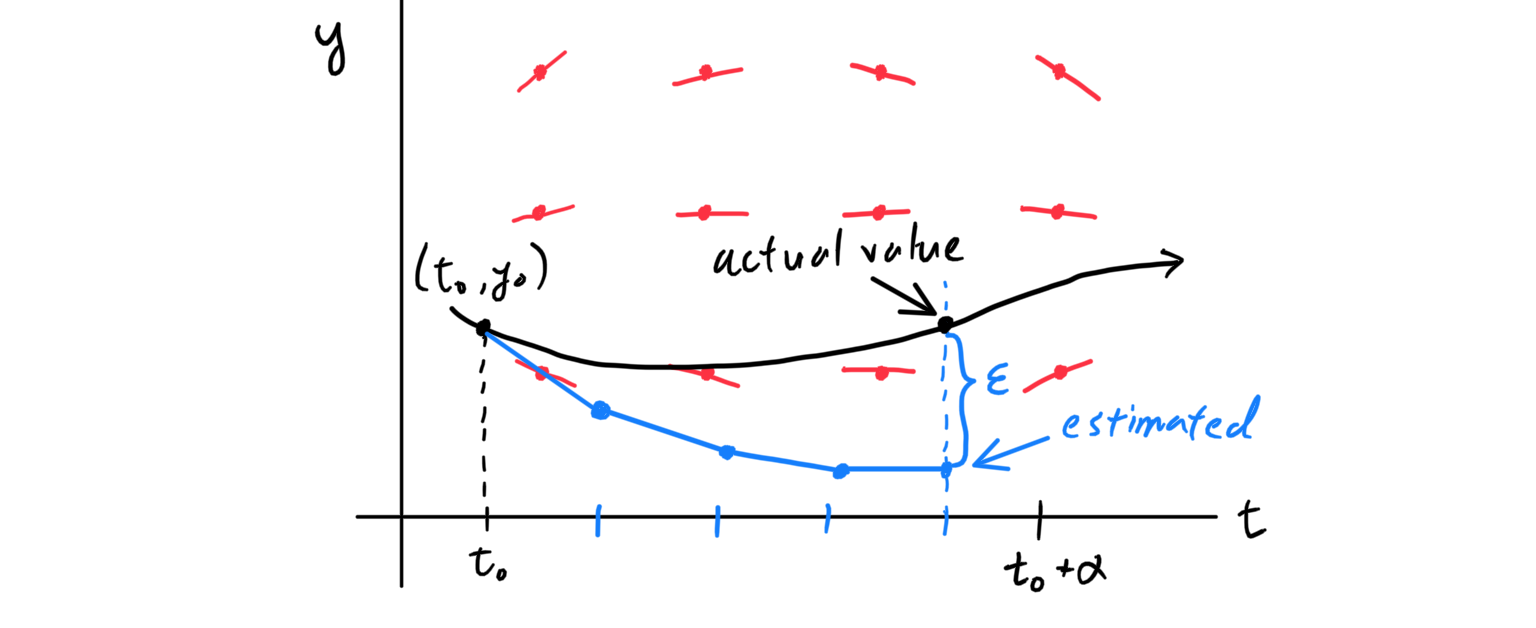
\includegraphics[scale=0.27]{img/Euler_Algorithm.PNG}
    \end{center}
    \end{definition}

    \begin{theorem}[Error Bound for Euler's Algorithm]
    The cumulative error bound for Euler's algorithm is
    \[\sum_{k=1}^n |T_k| = \frac{1}{2} M h^2 n = \frac{1}{2} \alpha M h\]
    \end{theorem}
    \begin{proof}
    Let $\varphi(t)$ be the exact solution. At $(t_k, y_k)$ and $(t_{k+1}, y_{k+1})$, 
    \[\varphi(t_{k+1}) = \varphi(t_k) + \int_{t_k}^{t_{k+1}} f\big(t, \varphi(t)\big) \, dt\]
    The formula for the approximate solution is
    \[y_{k+1} = y_k + (t_{k+1} - t_k) f(t_k, y_k)\]
    Therefore, the local error per point is 
    \begin{align*}
        T_k & \equiv |\varphi(t_{k+1}) - y_{k+1}| \\
        & = \bigg| \int_{t_k}^{t_{k+1}} f\big(t, \varphi(t)\big)\, dt - (t_{k+1} - t_k) f(t_k, y_k) \bigg| 
    \end{align*}
    We wish to establish an upper bound on $T_k$. For convenience of notation, let us denote $F(t) = f\big(t, \varphi(t)\big)$. This means that 
    \[T_k = \bigg| \int_{t_k}^{t_{k+1}} F(t)\,dt - (t_{k+1} - t_k ) F(t_k) \bigg| \]
    The mean value theorem says that there exists some $s_k \in (t_k, t)$ such that 
    \[F(t) - F(t_k) = (t - t_k) F^\prime (s_k)\]
    which implies that
    \begin{align*}
        \int_{t_k}^{t_{k+1}} F(t)\, dt & = \int_{t_k}^{t_{k+1}} F(t_k) + (t - t_k) F^\prime (s_k)\,dt \\
        & = \int_{t_k}^{t_{k+1}} (t - t_k) F^\prime (s) \, dt + (t_{k+1} - t_k) F (t_k) \\
        \implies & T_k = \bigg| \int_{t_k}^{t_{k+1}}  (t - t_k) F^\prime (s_k)\, dt \bigg|
    \end{align*}
    Let 
    \[M \equiv \max_{t_0 \leq t \leq t_0 + \alpha} \big| F^\prime (t) \big|\]
    Then, 
    \begin{align*}
        F^\prime (t) & = \frac{\partial F}{\partial t} \big(t, \varphi(t)\big) + \bigg( \frac{\partial F}{\partial y} \big(t, \varphi(t)\big) \bigg) \cdot \varphi^\prime (t) \\
        & = \frac{\partial F}{\partial t} \big(t, \varphi (t)\big) + \bigg(\frac{\partial F}{\partial y} \big(t, \varphi(t)\big) \bigg) f \big(t, \varphi(t)\big)
    \end{align*}
    Using the triangle inequality, we get
    \[M \leq \max_R \Big| \frac{\partial F}{\partial t} (t, y)\Big| + \max_R \Big| \frac{\partial F}{\partial y} (t, y)\Big| \cdot \max_R \Big| f(t, y) \Big|\]
    This means that the bound for $M$ can be calculated explicitly with the inequality above. It can be checked that
    \[M \leq \int_{t_k}^{t_{k+1}} (t - t_k) \, dt = \frac{M}{2}(t_{k+1} - t_k)^2 \]
    Assuming equal subdivisions, we can let $t_{k+1} - t_k = h = \frac{\alpha}{n}$ and conclude that 
    \[T_k \leq \frac{1}{2} M h^2\]
    Therefore, the cumulative error bound is 
    \[\sum_{k=1}^n |T_k| = \frac{1}{2} M h^2 n = \frac{1}{2} \alpha M h\]
    \end{proof}

\section{Linear Differential Equations}

  \begin{definition}[nth Order Linear DEQ]
  A \textit{$n$th order linear differential equation} has the form
  \[a_0 (t) y^{(n)} + a_1 (t) y^{(n-1)} + \ldots + a_{n-1} (t) y^\prime + a_n (t) y = f(t)\]
  where $a_0, a_1, \ldots, a_n, f \in C^0$ over interval $I \subset \mathbb{R}$. Using the linear operator 
  \[\mathcal{L}_n : C^n (\mathbb{R}) \longrightarrow C^0 (\mathbb{R}), \; \mathcal{L}_n (y) \equiv a_0 y^{(n)} + a_1 y^{(n-1)} + \ldots + a_{n-1} y^\prime + a_n y\]
  where 
  \[\mathcal{L}_n (y) (t) \equiv \bigg( \sum_{i=0}^n a_i y^{(n-i)} \bigg) (t) = \sum_{i=0}^n a_i (t) y^{(n-i)} (t)\]
  the DEQ can be written as
  \[\mathcal{L}_n (y) (t) = f(t), \text{ or } \mathcal{L}_n (y) = f\]
  The DEQ is said to be \textit{homogeneous} iff $f = 0$ and \textit{inhomogeneous} iff $f \neq 0$. 
  \end{definition}

  In general linear differential equations are important since it is often the case that we reduce nonlinear differential equations to linear ones with approximations. For example, the equation for the pendulum is approximated as
  \[\frac{d^2 \theta}{d t^2} + \frac{g}{L} \sin{\theta} = 0 \implies \frac{d^2 \theta}{d t^2} + \frac{g}{L} \theta = 0\]
  for small $\theta$. 

  \begin{example}
  Consider the equation 
  \[t y^{\prime \prime} + \cos{(t)} y^\prime + \Big( 1 - \frac{1}{1+t}\Big) y = 2t\]
  $1 - \frac{1}{1+t}$ is discontinuous at $t_0 = -1$, and this equation is not of second order at $t=0$. Therefore, valid intervals $I$ must be a subset of 
  \[(-\infty, -1) \cup (-1, 0) \cup (0, \infty)\]
  for which there exists a unique solution. 
  \end{example}

  \subsection{Solving Homogeneous Linear DEQs}

    This entire section is grounded in this theorem. 
    \begin{theorem}[The Fundamental Set]
    It can be seen that the set of functions $y = \varphi(t)$ that are solutions to the homogeneous equation $\mathcal{L}_n (y) = 0$ is simply just the kernel of $\mathcal{L}_n$, which is a subset of $C^n (\mathbb{R})$. Then, 
    \[\dim \ker{\mathcal{L}} = n \]
    The basis of $\ker{\mathcal{L}}$ is called the \textit{fundamental set}, and given that $\{\varphi_1, \varphi_2, \ldots, \varphi_n\}$ is this basis, the general solution is a linear combination of them. 
    \[\varphi = \sum_i k_i \varphi_i, \;\;\; k_i \in \mathbb{R}\]
    \end{theorem}

    This reduces the problem of finding a general solution to just finding $n$ linearly independent ones. 

    \begin{definition}[Wronskian]
    Let $f_1, f_2, \ldots, f_n$ be of class $C^{n-1} (\mathbb{R})$ in interval $I \subset \mathbb{R}$. Then, the \textit{Wronskian} is defined
    \[W(f_1, f_2, \ldots, f_n) \equiv \det{\begin{pmatrix}
    f_1&\ldots&f_n\\
    \vdots&\ddots&\vdots\\
    f_1^{(n-1)}&\ldots&f_n^{(n-1)}
    \end{pmatrix}}\]
    \end{definition}

    A simple application of the Wronskian is shown. 
    \begin{theorem}
    Let $\varphi_1, \varphi_2, \ldots, \varphi_n$ be any $n$ special solutions of the $n$th order linear homogeneous equation $\mathcal{L}(y) = 0$. Then, the set is linearly independent if and only if 
    \[W(\varphi_1, \ldots, \varphi_n) \neq 0\]
    Note that this theorem only works when the $\varphi_i$'s are known to be solutions. 
    \end{theorem}
    \begin{proof}
    Suppose that $W(\varphi_1, \ldots, \varphi_n) (t) \neq 0$ for all $t \in I$ and that $\varphi_1, \ldots, \varphi_n$ are linearly dependent. This means that there exists a nontrivial linear combination summing up to $0$, and differentiating the equation on both sides gives the following (by abuse of notation, we will denote $W$ as the Wronskian matrix, not the determinant): 
    \begin{align*}
        W(\varphi_1, \ldots, \varphi_n) \begin{pmatrix}
        b_1 \\ b_2 \\ \vdots \\ b_n \end{pmatrix} = \begin{pmatrix}
        0 \\ 0 \\ \vdots \\ 0 \end{pmatrix} \iff
        \begin{cases}
        b_1 \varphi_1 (t) + b_2 \varphi_2 (t) + \ldots + b_n \varphi_n (t) = 0 \\
        b_1 \varphi^\prime_1 (t) + b_2 \varphi^\prime_2 (t) + \ldots + b_n \varphi^\prime_n (t) = 0 \\
        \ldots \\
        b_1 \varphi^{(n-1)}_1 (t) + \ldots + b_n \varphi^{(n-1)}_n (t) = 0 
        \end{cases}
    \end{align*}
    For each fixed $t \in I$, by hypothesis $W$ is nonsingular, meaning that the only solution satisfying $W b = 0$ is when $b = 0$ itself. But this contradicts our assumption that $b \neq 0$, and so we have proved that
    \[W(\varphi_1, \ldots, \varphi_n) \neq 0 \implies \varphi_1, \ldots, \varphi_n \text{ linearly independent}\]
    Now, given that $W(\varphi_1, \ldots, \varphi_n) (t) = 0$ for some $t_0 \in I$, assume that $\varphi_1, \ldots, \varphi_n$ are linearly independent. $W(\varphi_1, \ldots, \varphi_n)(t_0)$ (interpreted as a matrix) is singular, the kernel of $W(\varphi_1, \ldots, \varphi_n)(t_0)$ is nontrivial; that is, there exists a nontrivial solution $b \neq 0$ to 
    \[W(\varphi_1, \ldots, \varphi_n)(t_0) \begin{pmatrix}
    b_1 \\ \vdots \\ b_n \end{pmatrix}= \begin{pmatrix} 
    0 \\ \vdots \\ 0 \end{pmatrix}\]
    To show linear dependence of the $\varphi_i$'s, we define a solution $\psi$ of the DEQ above as
    \[\psi (t) = b_1 \varphi_1 (t) + b_2 \varphi_2 (t) + \ldots + b_n \varphi_n (t)\]
    where $(b_1, \ldots, b_n)^T$ is any solution of $W(t_0) b = 0$ above. Since the system above tells us that
    \[\psi(t_0) = 0, \psi^\prime (t_0) = 0, \ldots, \psi^{(n-1)} (t_0) = 0\]
    it follows that $\psi= 0$ for all $t \in I$ is a solution. This means that we have found $b_1, \ldots, b_n$ such that 
    \[\psi = \sum_{i=1}^n b_i \varphi_i (t) = 0\]
    contradicting the assumption that $\varphi_i$'s were linearly independent. Therefore, 
    \[W(\varphi_1, \ldots, \varphi_n) = 0 \text{ for some } t_0 \in I \implies \varphi_1, \ldots, \varphi_n \text{ linearly dependent}\]
    \end{proof}

    \subsubsection{Homogeneous Equations with Constant Coefficients}

      Let us have the $n$th order linear homogeneous equation with constant coefficients $k_i \in \mathbb{R}$. 
      \[\mathcal{L}_n (y) \equiv k_0 y^{(n)} + k_1 y^{(n-1)} + \ldots + k_{n-1} y^\prime + k_n y = 0\]
      Now, assume that a solution in the form $e^{zt}$ is valid for $z \in \mathbb{C}$ (explained later). Then, 
      \begin{align*}
          \mathcal{L}(e^{zt}) & = k_0 (e^{zt})^{(n)} + k_1 (e^{zt})^{(n-1)} + \ldots + k_{n-1} (e^{zt})^\prime + k_n (e^{zt}) \\
          & = k_0 z^n e^{zt} + k_1 z^{n-1} e^{zt} + \ldots + k_{n-1} z e^{zt} + k_n e^{zt} \\
          & = e^{zt} \big( k_0 z^n + k_1 z^{n-1} + \ldots + k_{n-1} z + k_n \big) = 0
      \end{align*}

      \begin{definition}[Characteristic Polynomial]
      Given the linear DEQ $\mathcal{L}_n (y) = 0$, the \textit{characteristic polynomial} of $\mathcal{L}_n$ is 
      \[\sum_{i=0}^n k_i z^{n-i}\]
      \end{definition}

      Since $e^{zt} \neq 0$ for all values of $z$, we must find all zeroes of the characteristic polynomial. By the fundamental theorem of algebra, there exists $n$ solutions in $\mathbb{C}$, but it turns out that we can turn them into real solutions using the following lemma. 

      \begin{lemma}
      Given that we have complex valued solution $\varphi$ to $\mathcal{L}(y) = 0$, where
      \[\varphi = e^{z^* t} = e^{(\alpha + \beta i) t} = e^{\alpha t} \big(\cos{\beta t} + i \sin{\beta t}\big)\]
      and $z^*$ is a complex solution to the characteristic polynomial, the functions 
      \begin{align*}
          \text{Re}(\varphi) & = e^{\alpha t} \cos{\beta t} \\
          \text{Com}(\varphi) & = e^{\alpha t} \sin{\beta t} 
      \end{align*}
      are real solutions to the DEQ. 
      \end{lemma}
      \begin{proof}
      Since $z^* = \alpha + \beta i$ is a zero of the polynomial, its complex conjugate $\overline{z^*} = \alpha - \beta i$ is also a zero, meaning that the following two functions are solutions. 
      \begin{align*}
          \varphi & = e^{(\alpha + \beta i)t} = e^{\alpha t} \big( \cos{\beta t} + i \sin{\beta t}\big) \\
          \overline{\varphi} & = e^{(\alpha - \beta i)t} = e^{\alpha t} \big(\cos{\beta t} - i \sin{\beta t}\big) 
      \end{align*}
      By linearity of $\ker{\mathcal{L}}$, the following are also solutions
      \[\text{Re}(\varphi) = \frac{\varphi + \overline{\varphi}}{2}, \;\; \text{Com}(\varphi) = \frac{\varphi - \overline{\varphi}}{2}\]
      \end{proof}

      \begin{lemma}
      Given differential equation $\mathcal{L}(y) = 0$, let its characteristic polynomial have real root $z^*$ with multiplicity $m > 1$. Then, all the following are also real solutions of the DEQ:  
      \[e^{z^* t}, t e^{z^* t}, t^2 e^{z^* t}, \ldots, t^{m-1} e^{z^* t}\]
      If this root $z^*$ is complex then its complex conjugate $\overline{z^*}$ must also be a root of multiplicity $m$, and so in addition to $e^{z^* t}, \ldots, t^{m-1} e^{z^* t}$, the following are also (complex) solutions of $\mathcal{L}(y) = 0$. 
      \[e^{\overline{z^*} t} = \overline{e^{z^* t}}, \; t e^{\overline{z^*} t} = \overline{t e^{z^* t}}, \; t^2 e^{\overline{z^*} t} = \overline{t^2 e^{z^* t}}, \; \ldots, t^{m-1} e^{\overline{z^*} t} = \overline{t^{m-1} e^{z^* t}}\]
      and we can construct a basis of real-valued functions from these $2 (m-1)$ functions. 
      \begin{align*}
          &\text{Re}(e^{z^* t}), \text{Re}(t e^{z^* t}), \text{Re}(t^2 e^{z^* t}), \ldots,  \text{Re}(t^{m-1} e^{z^* t}) \\
          &\text{Com}(e^{z^* t}), \text{Com}(t e^{z^* t}), \text{Com}(t^2 e^{z^* t}), \ldots, \text{Com}(t^{m-1} e^{z^* t})
      \end{align*}
      \end{lemma}

      We can summarize all this in the following theorem. 

      \begin{theorem}[Solving Homogeneous Linear DEQs with Constant Coefficients]
      Let
      \[L_n (y) \equiv \sum_{i=0}^n a_i y^{(n-i)} = a_0 y^{(n)} + a_1 y^{(n-1)} + ... + a_{n-1} y^\prime + a_n y = 0, \; a_i \in \mathbb{R} \]
      be a $n$th order linear DEQ with constant coefficients and let
      \[p_n (z) = a_0 z^n + a_1 z^{n-1} + \ldots + \ldots + a_{n-1} z + a_n\]
      be its characteristic polynomial with distinct roots $z_1, z_2, \ldots, z_s (s \leq n)$, each root $z_i \in \mathbb{C}$ having multiplicity $m_i$. Note that $\sum_j m_j = n$ and 
      \[p_n (z) = \prod_{i=1}^s (z - z_i)^{m_i}\]
      Then, the $n$ functions form the complex fundamental set of the solutions of $\mathcal{L}_n (y) = 0$. 
      \begin{align*}
          \{ e^{z_1 t}, t e^{z_1 t}, ..., t^{m_1 - 1} e^{z_1 t},  \\
          e^{z_2 t}, t e^{z_2 t}, ..., t^{m_2 - 1} e^{z_2 t}, \\
          ................................... \\
          e^{z_s t}, t e^{z_s t}, ..., t^{m_s - 1} e^{z_s t}
      \end{align*}
      If any function $t^w e^{z_v t}$ (for $0 \leq w \leq m_s - 1, 1 \leq v \leq s$) is complex, then its conjugate $\overline{t^w e^{z_v t}}$ is also in the fundamental set and we can change the basis of the span of complex functions into the following basis of real functions having the same span:
      \[\{t^w e^{z_v t}, \overline{t^w e^{z_v t}}\} \implies \{\text{Re}(t^w e^{z_v t}), \text{Com}(t^w e^{z_v t})\}\]
      \end{theorem}

      \begin{example}
      The solutions to the equation $y^{\prime \prime} + y^\prime + y = 0$ is 
      \[\varphi_1 (t) = \exp \Big(\frac{-1+i\sqrt{3}}{2} t \Big), \;\; \varphi_2 (t) = \exp \Big( \frac{-1 - i \sqrt{3}}{2} t\Big) \]
      This implies, by the previous theorem, that the fundamental set of real solutions is
      \begin{align*}
          Re \big(\varphi_1 (t)\big) & = Re \bigg( e^{-\frac{1}{2} t} \Big( \cos{\Big(\frac{\sqrt{3}}{2}\Big)} + i \sin{\Big(\frac{\sqrt{3}}{2}\Big)}\Big) t\bigg) \\
          & = e^{-\frac{1}{2} t} \cos{\Big(\frac{\sqrt{3}}{2} t\Big)}  \\
          Com \big(\varphi_1 (t)\big) & = e^{-\frac{1}{2} t} \sin{\Big(\frac{\sqrt{3}}{2} t\Big)} 
      \end{align*}
      \end{example}

      We state the 2nd-order case separately since it is seen often in physical phenomena. 

      \begin{corollary}[Solutions to 2nd-Order Linear DEQs]
      Every solution $\varphi$ of $y^{\prime\prime} + py^\prime + q y = 0$ with $p, q \in \mathbb{R}$ and $p^2 \neq 4 q$ is defined on $-\infty < t < \infty$ and has the form 
      \[\varphi(t) = c_1 e^{z_1 t} + c_2 e^{z_2 t}\]
      where $z_1, z_2$ are roots of the equation $z^2 + p z + q = 0$. Furthermore, 
      \begin{enumerate}
          \item If $p^2 > 4q$, then $z_1, z_2 \in \mathbb{R}$ and are distinct. 
          \item If $p^2 < 4q$, then $z_1, z_2 \in \mathbb{C}$ with $z_1 = \bar{z_2} \implies$ if $z_1 = \alpha +\beta i$ is a solution, a general solution can be expressed 
      \[\varphi(t) = e^{\alpha t} \big( a_1 \cos{\beta(t)} + a_2 \sin{\beta(t)}\big)\]
          \item If $p^2 = 4q$, then $z^2 + p q + p = 0$ has a double root at $z = -\frac{p}{2} \implies$ a solution is $e^{- \frac{p}{2} t}$. The other solution is of the form, $t e^{- \frac{p}{2} t}$, making the general solution 
          \[(a_1 + a_2 t) e^{-\frac{p}{2} t}\]
      \end{enumerate}
      \end{corollary}
      \begin{proof}
      (1) and (2) are quite trivial. For (3), we know that $\varphi(t) = e^{-\frac{p}{2} t}$ is a solution, and we will try to construct another linearly independent solution. This important process that we will employ is analogous to the \textit{reduction of order} process that will be explained later. We assume that the second solution is of form
      \[\psi (t) = e^{-\frac{p}{2} t} w (t)\]
      Assume that $\psi (t)$ is a solution of $y^{\prime\prime} + p y^\prime + q y = 0$. Then manually differentiating, we get 
      \begin{align*}
          \psi (t) & = e^{-\frac{p}{2}t} w(t) \\
          \psi^\prime (t) & = e^{-\frac{p}{2} t} w^\prime (t) - \frac{p}{2} e^{-\frac{p}{2} t} w(t) \\
          \psi^{\prime\prime} (t) & = e^{-\frac{p}{2} t} w^{\prime \prime} (t) - p e^{-\frac{p}{2} t} w^\prime (t) + \frac{p^3}{4} e^{-\frac{p}{2} t} w(t) 
      \end{align*}
      Plugging these into the differential equation and simplifying gives us
      \begin{align*}
          \psi^{\prime\prime} (t) + p \psi^\prime (t) + q \psi (t) & = e^{-\frac{p}{2} t} \bigg( w^{\prime\prime} (t) + \Big( q - \frac{p^2}{4} \Big) w(t) \bigg) \\
          & = e^{-\frac{p}{2} t} w^{\prime\prime} (t) = 0
      \end{align*}
      Note that by hypothesis, $p^2 = 4q$. Since $e^{-\frac{p}{2} t} \neq 0$, 
      \[w^{\prime\prime} (t) = 0 \implies w (t) = a_1 + a_2 t \implies \psi(t) = e^{-\frac{p}{2} t} (a_1 + a_2 t)\]
      \end{proof}

    \subsubsection{Reduction of Order}

      We elaborate on the method used in the previous section and introduce the reduction of order method. 

      \begin{theorem}[Reduction of Order of 2nd-Order Linear DEQs]
      Given the homogeneous linear differential equation with nonconstant coefficients 
      \[\mathcal{L}_2 (y) = a_0 (t) y^{\prime\prime} + a_1 (t) y^\prime + a_2 (t) y = 0\]
      where $a_0, a_1, a_2$ are $C^0$ on $I$ and $a_0 (t) \neq 0$ on $I$, assume that we know a solution $\varphi_1$. Then, the second solution is
      \[\varphi_2 (t) = \varphi_1 (t) \int_{t_0}^t \frac{1}{\varphi_1^2 (\sigma)} \exp \bigg(- \int_{t_0}^\sigma \frac{a_1 (s)}{a_0 (s)}\,ds \bigg) \, d\sigma\]
      \end{theorem}
      \begin{proof}
      Since we know solution $\varphi_1$, we assume that the second solution is of form $\varphi_2 (t) = w (t) \varphi_1 (t)$ and try to find a nonconstant function satisfying the DEQ. Since,
      \begin{align*}
          \varphi_2 & = w \varphi_1 \\
          \varphi_2^\prime & = w^\prime \varphi_1 + w \varphi_1^\prime \\
          \varphi_2^{\prime\prime} & = w^{\prime\prime} \varphi_1 + 2 w^\prime \varphi_1^\prime + w \varphi_1^{\prime\prime}
      \end{align*}
      We have
      \[\mathcal{L}_2 (\varphi_2) = a_0 \varphi_1 w^{\prime\prime} + (2 a_0 \varphi_1^\prime + a_1 \varphi_1) w^\prime + w \mathcal{L}_2 (\varphi_1) \text{ for all } t \in I\]
      But since $\mathcal{L}_2 (\varphi_1) = 0$, 
      \[\mathcal{L}_2 (\varphi_2) = a_0 \varphi_1 w^{\prime\prime} + (2 a_0 \varphi_1^\prime + a_1 \varphi_1) w^\prime\]
      But notice that this is a first-order linear equation in $w^\prime$! What we have essentially done is use the fact that $\mathcal{L}_2 (\varphi_1) = 0$ to "reduce" the the DEQ from a second-order equation to a first-order one. Letting $v = w^\prime$ gives 
      \[v^\prime + \bigg( 2 \frac{\varphi_1^\prime}{\varphi_1} + \frac{a_1}{a_0} \bigg) v = 0\]
      Separating variables we obtain the solution
      \[v(t) = \frac{1}{\varphi_1^2 (t)} \exp \bigg(- \int_{t_0}^t \frac{a_1(s)}{a_0 (s)} \,ds \bigg) \implies w(t) = \int_{t_0}^t \frac{1}{\varphi_1^2 (\sigma)} \exp \bigg(- \int_{t_0}^\sigma \frac{a_1(s)}{a_0 (s)} \,ds \bigg) \,d\sigma \]
      \end{proof}

      This process can be repeated for higher order equations, we show it for 3rd-order equations. 

      \begin{theorem}[Reduction of Order of 3rd-Order DEQs]
      Given the homogeneous linear differential equation with nonconstant coefficients
      \[\mathcal{L}_3 (y) = a_0 (t) y^{\prime\prime\prime} + a_1 (t) y^{\prime\prime} + a_2 (t) y^\prime + a_3 (t) y = 0\]
      where $a_0, a_1, a_2, a_3$ are $C^0$ on $i$ and $a_0 (t) \neq 0$ on $I$, assume that we know a solution $\varphi_1$. Then, the second and third solutions are
      \[\varphi_2 = \varphi_1 \int_{t_0}^t \gamma_1(s)\,ds, \;\;\varphi_3 = \varphi_1 \int_{t_0}^t \gamma_2(s)\,ds\]
      where $\gamma_1, \gamma_2$ are the solutions of differential equation
      \[a_0 \varphi_1 v^{\prime\prime} + (3a_0 \varphi_1^\prime + a_1 \varphi_1) v^\prime + (3 a_0 \varphi_1^{\prime\prime} + 2a_1 \varphi_1^\prime + a_2 \varphi_1) v = 0\]
      \end{theorem}
      \begin{proof}
      We assume that the second solution is of form $\varphi_2 (t) = w(t) \varphi_1(t)$ and compute the derivatives 
      \begin{align*}
          \varphi_2 & = w \varphi_1 \\
          \varphi_2^\prime & = w^\prime \varphi_1 + w \varphi_1^\prime \\
          \varphi_2^{\prime\prime} & = w^{\prime\prime} \varphi_1 + 2 w^\prime \varphi_1^\prime + w \varphi_1^{\prime\prime} \\
          \varphi_2^{\prime\prime\prime} & = w^{\prime\prime\prime} \varphi_1 + 3 w^{\prime\prime} \varphi_1^\prime + 3 w^\prime \varphi_1^{\prime\prime} + w \varphi_1^{\prime\prime\prime}
      \end{align*}
      Substituting these into $\mathcal{L}_3 = 0$ and simplifying gives
      \[\mathcal{L}_3 (\varphi_2) = a_0 \varphi_1 w^{\prime\prime\prime} + (3a_0 \varphi_1^\prime + a_1\varphi_1) w^{\prime\prime} + (3 a_0 \varphi_1^{\prime\prime} + 2a_1 \varphi_1^\prime + a_2 \varphi_1) w^\prime + w \mathcal{L}_3 (\varphi_1) \text{ for all } t\in I\]
      Again, since $\mathcal{L}_3 (\varphi_1) = 0$, we get
      \[\mathcal{L}_3 (\varphi_2) = a_0 \varphi_1 w^{\prime\prime\prime} + (3a_0 \varphi_1^\prime + a_1\varphi_1) w^{\prime\prime} + (3 a_0 \varphi_1^{\prime\prime} + 2a_1 \varphi_1^\prime + a_2 \varphi_1) w^\prime\]
      which is really just a 2nd order equation in $w^\prime$. Substituting $v = w^\prime$ gives us
      \[\mathcal{L}_3 (\varphi_2) = a_0 \varphi_1 v^{\prime\prime} + (3a_0 \varphi_1^\prime + a_1 \varphi_1) v^\prime + (3 a_0 \varphi_1^{\prime\prime} + 2a_1 \varphi_1^\prime + a_2 \varphi_1) v \]
      Therefore, we have successfully reduced the order of this DEQ. Upon finding the two solutions $\gamma_1, \gamma_2$, the solution will be of form 
      \[\varphi_2 = \varphi_1 \int_{t_0}^t \gamma_1(s)\,ds, \;\;\varphi_3 = \varphi_1 \int_{t_0}^t \gamma_2(s)\,ds\]
      \end{proof}

    \subsubsection{Cauchy-Euler's Equation}

      \begin{definition}
      A \textit{Cauchy-Euler equation of order $n$} has the form 
      \[t^n y^{(n)} + a_1 t^{n-1} y^{(n-1)} + a_2 t^{n-2} y^{(n-2)} + ... + a_{n-1} t y^\prime + a_n y = 0, \;\; a_i \in \mathbb{R}\]
      \end{definition}

      There are two ways we can explicitly solve for this equation. Since the most common Cauchy-Euler equation is the second-order one, we will solve the following 
      \[t^2 y^{\prime \prime} + a t y^\prime + b y = 0\]
      \begin{enumerate}
          \item A trial solution $y = t^m$ can be used to directly solve for basic solutions (guess and check method). We assume a trial solution $y = t^m$. Differentiating it gives
          \[y^\prime (t) = m t^{m-1}, \;\; y^{\prime\prime} (t) = m (m-1) t^{m-2}\]
          Substituting into the original equation and simplifying gives: 
          \[t^2 \big( m(m-1)t^{m-2}\big) + at \big( m t^{m-1}\big) + b \big( t^m \big) = 0 \implies m^2 + (a-1) m + b = 0\]
          There are three possible cases: 
          \begin{enumerate}
              \item Two distinct roots $m_1, m_2$: 
              \[y = c_1 x^{m_1} + c_2 x^{m_2}\]
              \item One repeated root $m$: 
              \[y = c_1 x^m \ln{x} + c_2 x^m\]
              Note that this solution is found using the reduction of order. 
              \item Complex conjugate roots $\alpha \pm \beta i$: 
              \[y = c_1 x^{\alpha} \cos(\beta \ln{x}) + c_2 x^\alpha \sin(\beta \ln{x})\] 
              This can be easily derived by using Euler's formula. 
          \end{enumerate}
          \item 
      \end{enumerate}


      Consider the equation of the form 

      We can use substitution $|t| = e^s$ to reduce the equation to have constant coefficients. 


      \begin{enumerate}
          \item $t > 0, t = e^s \implies s = \log(t), y(t) = y(e^s) = w(s) = w \big( \log(t)\big)$. This implies that
          \begin{align*}
              & \frac{d y}{d t} = \frac{dw}{ds} \frac{ds}{dt} = \frac{1}{t} \frac{dw}{ds} \\
              \implies & \frac{d^2 y}{dt^2} = -\frac{1}{t^2} \frac{dw}{ds} + \frac{1}{t} \frac{d}{dt} \bigg( \frac{dw}{ds}\bigg) = \frac{1}{t^2} \bigg( \frac{d^2 w}{ds^2} - \frac{dw}{ds} \bigg) \\
              \implies & \text{substituting, } \frac{d^2 w}{ds^2} - \frac{dw}{ds} + a_1 \frac{dw}{ds} + a_2 w(s) = 0 \\
              \implies & w^{\prime\prime} + (a_1 - 1) w^\prime + a_2 w = 0
          \end{align*}
          \item When $t<0$, the procedure is similar. 
      \end{enumerate}
      This results in the equation $L(w) =0$ having the general solution 
      \[\begin{cases}
      c_1 e^{z_1 s} + c_2 e^{z_2 s} & z_1 \neq z_2 \text{ roots of } z^2 + (a_1 - 1) z + a_2 = 0 \\
      (c_1 + c_2 s) e^{z_1 s} & z_1 = z_2 \text{ roots of ''}
      \end{cases}\]
      This means that the solution of $L(y) = 0$ is one of
      \[\begin{cases}
      \varphi(t) = c_1 |t|^{z_1} + c_2 |t|^{z_2} \\
      \varphi(t) = (c_1 + c_2 \log|t|) |t|^{z_1}
      \end{cases}\]
      If $t \in \mathbb{C}$, $e^{z \log|t|} = |t|^2$, assuming that $z = \alpha + \beta i$. This means that 
      \begin{align*}
          |t|^2 = e^{(\alpha + \beta i) \log|t|} & = e^{\alpha \log|t|} \big( \cos{(\beta \log|t|)} + i \sin{(\beta \log|t|)}\big) \\
          & = |t|^\alpha \big( \cos{(\beta \log|t|)} + i \sin{(\beta \log|t|)}\big)
      \end{align*}

  \subsection{Solving Inhomogeneous Linear DEQs}

    \begin{definition}[Inhomogeneous Linear DEQ]
    An \textit{inhomogeneous linear equation} is a linear differential equation in the form
    \[\mathcal{L}_n (y) = f\]
    where $f \neq 0$. $f \neq 0$ usually denotes that there is an external force acting on the system. 
    \end{definition}

    \begin{example}[Dampened Linear Mass-Spring System with Periodic External Force]
    The dampened linear mass-spring system subjected to given periodic external force $A \cos{\omega t}$ is represented by the linear DEQ
    \[y^{\prime \prime} + by^\prime + \frac{k}{m} y = \frac{A}{M} \cos{\omega t}\]
    \end{example}

    The following theorem provides insight into the structure of the solutions for these systems. 
    \begin{theorem}
    Suppose $\psi_p$ is a particular solution of $\mathcal{L}_n (y) = f$ on $I$ and suppose $\varphi_1, \varphi_2, ..., \varphi_n$ are $n$ linearly independent solutions of the homogeneous equation 
    \[\mathcal{L}_n (y) = 0\]
    Then, every solution $\psi$ of $\mathcal{L}_n (y) = f$ has general form
    \[\psi = \psi_p + \sum_{i=1}^n c_i \varphi_i\]
    That is, the set of all solutions is an $n$ dimensional affine subspace within the space of all continuous functions. 
    \end{theorem}
    \begin{proof}
    Let $\psi_p$ be a particular solution of $\mathcal{L}_n (y) = f$ and $\psi_0$ be any solution of $\mathcal{L}_n (y) = 0$. Then, $\psi_0 \in \ker{\mathcal{L}_n}$, which means that by linearity of $\mathcal{L}_n$, 
    \[\mathcal{L}_n (\psi_p + k \psi_0) = \mathcal{L}_n (\psi_p) + k \mathcal{L}_n (\psi_0) = f + 0 = f\]
    \end{proof}

    We have reduced the problem of solving inhomogeneous DEQs into solving the homogeneous version and finding a particular solution. 

    \subsubsection{Variation of Constants}

      We now attempt to find a particular solution $\psi_p$ for a second order linear inhomogeneous equation. The great thing about the method below is that as long as the functions $a_0 \neq 0, a_1, a_2, f$ are continuous over certain interval $I \subset \mathbb{R}$, it always provides us with a specific solution. 

      \begin{theorem}[Variation of Constants Formula for 2nd-Order Linear DEQs]
      Given inhomogeneous linear DEQ
      \[\mathcal{L}_2(y) = a_0 (t) y^{\prime \prime} + a_1 (t) y^\prime + a_2 (t) y = f\]
      where $a_0, a_1, a_2, f$ are all continuous on $I$, assume that we have the general solution $\varphi = c_1 \varphi_1 + c_2 \varphi_2$ for $\mathcal{L}_2(y) = 0$. Then, a particular solution $\psi_p$ for $\mathcal{L}_2 (y) = f$ is given by the \textit{Variation of Constants formula} 
      \begin{align*}
          \psi_p & = \varphi_1 (t) \Bigg( - \int_{t_0}^t \frac{f(s)\,\varphi_2 (s)}{ a_0 (s) W(\varphi_1, \varphi_2) (s)}\,ds \Bigg) + \varphi_2 (t) \Bigg( \int_{t_0}^t \frac{f(s)\,\varphi_1 (s)}{ a_0 (s) W(\varphi_1, \varphi_2) (s)}\,ds \Bigg) \\
          & = \psi_p (t) = \int_{t_0}^t \frac{f(s) \, \big( \varphi_2 (t) \varphi_1 (s) - \varphi_1(t) \varphi_2 (s)\big)}{a_0 (s) \, W(\varphi_1, \varphi_2) (s)}\,ds
      \end{align*}
      \end{theorem}
      \begin{proof}
      We assume that the particular solution is of the form 
      \[\psi_p = u_1 \varphi_1 + u_2 \varphi_2\]
      and that we have found these functions $u_1, u_2$. This assumption is quite arbitrary, but we will see why this works later. This implies that
      \begin{align*}
          &\psi_p^\prime = (u_1 \varphi_1 + u_2 \varphi_2)^\prime  = u_1 \varphi_1^\prime + u_2 \varphi_2^\prime + u_1^\prime \varphi_1 + u_2^\prime \varphi_2 \\
          & \psi_p^{\prime \prime} = u_1 \varphi_1^{\prime \prime} + u_2 \varphi_2^{\prime \prime} + 2 u_1^\prime \varphi_1 + 2 u_2^\prime \varphi_2^\prime + u_1^{\prime \prime} \varphi_2 + u_2^{\prime \prime} \varphi_2
      \end{align*}
      With these derivatives, we can expand out the equation $\mathcal{L}_2 (\psi_p) = f$ to get
      \begin{align*}
          \mathcal{L}_2(\psi_p) = \mathcal{L}_2 (u_1 \varphi_1 + u_2 \varphi_2) & = a_0 (u_1 \varphi_1 + u_2 \varphi_2)^{\prime\prime} + a_1 (u_1 \varphi_1 + u_2 \varphi_2)^{\prime} + a_0 (u_1 \varphi_1 + u_2 \varphi_2) \\
          & = ... \\
          & = a_0 \big( (\varphi_1 u_1^{\prime\prime} + \varphi_2 u_2^{\prime \prime}) + 2(\varphi_1^\prime u_1^\prime + \varphi_2^\prime u_2^\prime)\big) + a_1 (\varphi_1 u_1^\prime + \varphi_2 u_2^\prime) = f
      \end{align*}
      We would like to obtain some sort of relation from this last equation. If we assume that 
      \[\varphi_1 u_1^\prime + \varphi_2 u_2^\prime = 0\]
      for all $t \in I$, then $(\varphi_1 u_1^\prime + \varphi_2 u_2^\prime)^\prime = \varphi_1 u_1^{\prime\prime} + \varphi_2 u_2^{\prime\prime} + \varphi_1^\prime u_1^{\prime} + \varphi_2^\prime u_2^{\prime} = 0$ and thus
      \[a_0 \big( (\varphi_1 u_1^{\prime\prime} + \varphi_2 u_2^{\prime \prime}) + 2(\varphi_1^\prime u_1^\prime + \varphi_2^\prime u_2^\prime)\big) + a_1 (\varphi_1 u_1^\prime + \varphi_2 u_2^\prime) = f \implies \varphi_1^\prime u_1^\prime + \varphi_2^\prime u_2^\prime = \frac{f}{a}\]
      Notice our line of reasoning so far: Assuming the existence of a solution of form $\psi_p = u_1 \varphi_1 + u_2 \varphi_2$ (and that $\varphi_1 u_1^\prime + \varphi_2 u_2^\prime = 0$) implies that $\varphi_1^\prime u_1^\prime + \varphi_2^\prime u_2^\prime = \frac{f}{a}$. However, we can reason backwards and state this: If we can find two equations $u_1, u_2$ satisfying $\varphi_1 u_1^\prime + \varphi_2 u_2^\prime = 0$ and $\varphi_1^\prime u_1^\prime + \varphi_2^\prime u_2^\prime = \frac{f}{a}$, then $\varphi_p = u_1 \varphi_2 + u_2 \varphi_2$ satisfies $\mathcal{L}_2 (\varphi_p) = f$ on $I$. So assume that there exists $u_1, u_2$ such that (written in matrix form)
      \[\begin{pmatrix}
      \varphi_1 & \varphi_2 \\
      \varphi_1^\prime & \varphi_2^\prime
      \end{pmatrix} \begin{pmatrix}
      u_1^\prime \\u_2^\prime
      \end{pmatrix} = \begin{pmatrix}
      0 \\ f / a_0
      \end{pmatrix}\]
      Using Cramer's rule, we solve for $u_1^\prime, u_2^\prime$ and integrate to get $u_1, u_2$. 
      \begin{align*}
          u_1^\prime = \frac{1}{W(\varphi_1, \varphi_2)} \det{\begin{pmatrix} 0 & \varphi_2 \\ f / a_0 & \varphi_2^\prime
          \end{pmatrix}} = \frac{-f \varphi_2}{a_0 W(\varphi_1, \varphi_2)} \implies u_1 (t) = \int_{t_0}^t \frac{-f(s)\,\varphi_2 (s)}{ a_0 (s) W(\varphi_1, \varphi_2) (s)}\,ds \\
          u_2^\prime = \frac{1}{W(\varphi_1, \varphi_2)} \det{\begin{pmatrix} \varphi_1 & \varphi_1^\prime \\ 0 & f / a_0
          \end{pmatrix}} = \frac{f \varphi_1}{a_0 W(\varphi_1, \varphi_2)} \implies u_2 (t) = \int_{t_0}^t \frac{f(s)\,\varphi_1 (s)}{ a_0 (s) W(\varphi_1, \varphi_2) (s)}\,ds
      \end{align*}
      Therefore, 
      \[\psi_p (t) = u_1 (t) \varphi_1 (t) + u_2 (t) \varphi_2 (t) = \int_{t_0}^t \frac{f(s) \, \big( \varphi_2 (t) \varphi_1 (s) - \varphi_1(t) \varphi_2 (s)\big)}{a_0 (s) \, W(\varphi_1, \varphi_2) (s)}\,ds\]
      \end{proof}


      \begin{theorem}[Variation of Constants Formula]
      For an $n$th order linear differential equation 
      \[\mathcal{L}_n (y) = a_0 (t) y^{(n)} + a_1 (t) y^{(n-1)} + \ldots + a_{n-1} (t) y^\prime + a_n (t) y = f\]
      Let the fundamental set of its homogeneous counterpart $\mathcal{L}_n (y) = 0$ be $\varphi_1, \ldots, \varphi_n$. Then, upon solving the system 
      \[\begin{pmatrix}
      \varphi_1 & \varphi_2 & \ldots & \varphi_n \\
      \varphi_1^\prime & \varphi_2^\prime & \ldots & \varphi_n^\prime\\
      \vdots & \vdots & \ddots & \vdots \\
      \varphi_1^{(n-1)} & \varphi_2^{(n-1)} & \ldots & \varphi_n^{(n-1)} 
      \end{pmatrix} \begin{pmatrix}
      u_1^\prime \\ u_2^\prime \\ \vdots \\ u_n^\prime 
      \end{pmatrix} = \begin{pmatrix}
      0 \\ \vdots \\ 0 \\ f / a_0
      \end{pmatrix}\]
      for $u_1^\prime, u_2^\prime, \ldots, u_n^\prime$, we find $\psi_p$ to be
      \[\psi_p (t) = \sum_{i=1}^n u_i (t) \varphi_i(t) = \sum_{i=1}^n \Big( \int_{t_0}^t u_i^\prime (s)\,ds \Big) \varphi_i (t)\]
      \end{theorem}

\section{Series Solutions of Linear Equations}

  A wider class of differential equations has solutions that can be expanded into a power series than ones that can be solved in closed form (that is, expressed in terms of elementary functions). 

  \begin{example}
  Given the differential equation
  \[y^{\prime \prime} = -\sin{(y)} - y^\prime, \; \varphi(0) = \frac{\pi}{4}, \varphi^\prime (0) = 0\]
  Assuming that $\varphi$ is an analytic function, we can write the Taylor series 
  \[\varphi(t) = \varphi(0) + \varphi^\prime (0) t + ... = \sum_{j=0}^\infty \frac{\varphi^{(j)} (0)}{j!} t^j\]
  We can solve for each derivative manually by plugging it into the equation
  \begin{align*}
      & \varphi^{\prime\prime} (0) = -\sin{\big( \varphi(0)\big)} - \varphi^\prime (0) = - \frac{\sqrt{2}}{2} \\
      & \varphi^{\prime\prime\prime} (0) = -\cos{\big(\varphi(0)\big)} \varphi^{\prime\prime}(0) - \varphi^{\prime\prime} (0) = \frac{\sqrt{2}}{2} \\
      & \varphi^{(4)} (0) = \sin{\Big(\varphi(0)\big)} \big( \varphi^\prime (0)\big)^2 - \cos{\Big(\varphi(0)\big)} \varphi^{\prime\prime} (0) - \varphi^{(3)} (0) = \frac{1-\sqrt{2}}{2}
  \end{align*}
  Doing this recursively, the expansion of the solution $\varphi$ begins with the terms 
  \[\varphi(t) = \frac{\pi}{4} - \frac{\sqrt{2}}{2} \frac{t^2}{2!} + \frac{\sqrt{2}}{2} \frac{t^3}{3!} + \frac{1-\sqrt{2}}{2} \frac{t^4}{4!} + ...\]
  \end{example}

  \subsection{Review of Power Series}

    Every power series 
    \[\sum_{n=0}^\infty c_n t^n\]
    has a radius of convergence $R \geq 0$ over $\mathbb{C}$. Some more properties: 
    \begin{enumerate}
        \item The series converges absolutely for $|t| < R$. 
        \item Assigning $f(t) = \sum c_n t^n$ for $|t| < R, f \in C^\infty$, then 
        \[f^{(k)}(t) = \sum_{n=k}^\infty \frac{n!}{k!} c_n t^{n-k}\]
        with radius of convergence also $R$.
        \item If $[a, b]$ is the interval of convergence, then 
        \[\int_a^b f(s) \,ds = \sum_{n=0}^\infty c_n \int_a^b s^n \, ds\]
        In particular, 
        \[\int_0^t f(s)\,ds = \sum_{n=0}^\infty \frac{c_n}{n+1} t^{n+1}\]
        which also has a radius of convergence $R$. 
        \item Identity theorem for power series. If $g(t) = \sum d_n t^n$ is another power series with ROC $= \Tilde{R}$, and $f(t) = g(t)$ on some interval in which the series both converge, then $d_n = c_n$ for all $n$. In particular, if the sum of a power series is $0$ for all $t \in I$, then every coefficient in the series must be $0$. 
        \item $f, g$ converge $\implies f+g$ converges within the ROC of both $f$ and $g$. 
        \item $f, g$ converges $\implies fg$ converges within the ROC of both $f$ and $g$. 
    \end{enumerate}

    \begin{definition}
    $f$ is \textit{analytic at $t=a$} if and only if it can be expanded into a Taylor series 
    \[f(t) = \sum_{n=0}^\infty c_n (t-a)^n, \;\; c_n = \frac{f^{(n)}(n)}{k!}\]
    with radius of convergence $R > 0$. 
    \end{definition}
    It is assumed that the reader is familiar with basic convergence tests such as the ratio test and the comparison test. 

    \begin{lemma}
    Let $f, g$ be analytic functions. That is, they can be expressed
    \[f(t) = \sum_{n=p}^\infty c_n (t-a)^n, \;\;\; g(t) = \sum_{n=q}^\infty d_n (t-a)^n\]
    Without loss of generality, suppose $p < q$ and $d_q \neq 0$. Then, $f$ and $g$ are linearly independent on every interval $I$ in which $f, g$ converges. 
    \end{lemma}
    \begin{proof}
    This proof is trivial using linear algebra since $f$ is expressed using more basis vectors. 
    \end{proof}

  \subsection{2nd Order Linear Equations w/ Analytic Coefficients}

    \begin{example}
    Despite what we have learned, the differential equation 
    \[y^{\prime\prime} (t) - t y = 0, \;\; \varphi(t_0) = a, \varphi^\prime (t_0) = b\]
    cannot be solved with any of the previous methods, but there does exist unique solutions for all $t$. We wish to find a solution using a new method. Assume that $\varphi(t)$ is analytic at $t= t_0$. That is, it can be expanded
    \[\varphi(t) = c_0 + c_1 (t-t_0) + c_2 (t-t_0)^2 + \ldots = \sum_{k=0}^\infty c_k (t-t_0)^k\]
    that converges in an interval $|(t-t_0)| < A$ (we will not worry about convergence yet). We can calculate
    \begin{align*}
        \varphi^{\prime\prime} (t) - t \varphi(t) & = \sum_{k=2}^\infty k(k-1) c_k (t-t_0)^{k-2} - \sum_{k=0}^\infty c_k (t-t_0)^{k+1} \\
        & = 2 c_2 + \sum_{k=3}^\infty \big( k(k-1) c_k - c_{k-3}\big) (t-t_0)^{k-2} = 0
    \end{align*}
    if and only if $\varphi(t)$ is a solution of $y^{\prime\prime} - t y = 0$. This implies that 
    \begin{align*}
        & 2 c_2 = 0, k(k-1) c_k - c_{k-3} = 0 \\
        \implies & c_2 = 0, c_3 = \frac{1}{2 \cdot 3} c_0, c_4 = \frac{1}{3 \cdot 4} c_1, c_5 = \frac{1}{4 \cdot 5} c_2, ... \\
        \implies & \begin{cases}
        c_{3m} = \frac{(1)(4)...(3m-2)}{(3m)!} c_0 \\
        c_{3m+1} = \frac{(2)(5)(8)...(3m-1)}{(3m+1)!} c_1 \\
        c_{3m+2} = 0
        \end{cases}
    \end{align*}
    which proves us an explicit definition of $\varphi$ dependent on initial conditions $a = \varphi(0) = c_0, b = \varphi^\prime (0) = c_1$. Therefore, a candidate for a solution is
    \begin{align*}
        \varphi(t) & = a \varphi_1 (t) + b \varphi_2 (t) \\
        & = a \bigg( 1 + \sum_{m=1}^\infty \frac{(1)(4)...(3m-2)}{(3m)!} (t-t_0)^{3m} \bigg) + b \bigg( 1 + \sum_{m=1}^\infty \frac{(2)(5)...(3m-1)}{(3m+1)!} (t-t_0)^{3m+1} \bigg)
    \end{align*}
    We can see that this infinite series converges for $|(t-t_0)| < \infty$. 
    \end{example}

    \begin{theorem}[Existence of Analytic Solutions of 2nd-Order Linear DEQs of Analytic Coefficients]
    Given equation (with leading coefficient $1$)
    \[y^{\prime\prime} + p(t) y + q(t) y = f(t)\]
    If $p, q, f$ are analytic at $t_0$, then there exists a unique solution $\varphi$ satisfying $\varphi (t_0) = a, \varphi^\prime (t_0) = b$. This solution is analytic at $t = t_0$, with expansion
    \[\varphi(t) = \sum_{k=0}^\infty c_k (t-t_0)^k\]
    converging for at least those values of $t$ converging on $p, q$ and $f$. The coefficients $c_k$ can be determined recursively by direct substitution into the differential equation. 
    \end{theorem}

    Notice that this series method can be very useful computationally. For values close to $t_0$, we can calculate the series up to a certain number of coefficients to gain a good approximation of the actual function. 

    \begin{example}[Legendre Equation]
    Given the equation
    \[(1 - t^2) y^{\prime \prime} - 2 t y^\prime + \alpha (\alpha + 1) y = 0\]
    with $\alpha$ a given constant. In order to determine whether this differential equation has a series solution about $t=0$, we use the previous theorem. We modify the equation to
    \begin{align*}
        y^{\prime\prime} - \frac{2 t}{1 - t^2} y^\prime + \frac{\alpha (\alpha + 1)}{1 - t^2} y = 0 \;\;\; (t \neq \pm 1) 
    \end{align*}
    The coefficient functions are indeed analytic. That is, 
    \begin{align*}
        & - \frac{2t}{1 - t^2} = -2 t (1 + t^2 + t^4 + ... ) = -2t \sum_{k=0}^\infty t^{2k} \\
        & \frac{\alpha(\alpha+1)}{1 - t^2} = \alpha (\alpha + 1) \sum_{k=0}^\infty t^{2k}
    \end{align*}
    with a radius of convergence of $1$. Therefore, the conditions of the theorem are satisfied, and the Legendre equation has a unique analytic solution satisfying $\varphi(0) = a, \varphi^\prime (0) = b$ for all $a, b$. 
    \end{example}

  \subsection{Singular Points of Linear Equations}

    Many differential equations which arise in applications, the so-called equations of mathematical physics, fail to satisfy the hypotheses of the theorem stating the existence of analytic solutions. That is, there are points $t = t_0$ where the coefficients are not analytic (usually because it is unbounded). They usually pop up when we divide the entire equation by the leading coefficient $a_0 (t)$, which leads to one of the non-leading coefficients to become un-analytic when it is of the form 
    \[\frac{a_i(t)}{a_0 (t)} \]
    We formalize this below 

    \begin{definition}[Singular Point]
    $t = t_0$ is a \textit{singular point} of the differential equation
    \[\mathcal{L}_n (y) = a_0 (t) y^{(n)} + a_1 (t) y^{(n-1)} + \ldots + a_{n-1} (t) y^\prime + a_n (t) y = 0\]
    if $a_0, a_1, \ldots, a_n$ are analytic at $t_0$ and $a_0 (t_0) = 0$, but $a_1, \ldots, a_n$ are not all zero at $t_0$. A point that is not a singular point is called an \textit{ordinary point}. 
    \end{definition}

    In relation to the theorem on the existence of analytic solutions, we would like to clarify that given singular point $t_0$ and non-singular point $t_1$, 
    \begin{align*}
        \text{At } t = t_1 & \implies \text{Analytic solution exists (theorem)} \\
        \text{At } t = t_0 & \implies \text{Analytic solution could exist or not} 
    \end{align*}
    That is, the theorem tells us that given equation
    \[y^{\prime\prime} + p(t) y + q(t) y = f(t)\]
    where $p, q, f$ are analytic at $t_1$ (i.e. $t_1$ is ordinary), we are guaranteed the existence of a analytic solution in a neighborhood of $t_1$. However, if $p, q$ are somehow not analytic, then there \textit{may or may not} be an analytic solution. This will be elaborated in the following example. 

    \begin{example}[Nonexistence of Analytic Solutions in 1st-Order Cauchy-Euler Equation]
    Consider the first-order Cauchy-Euler equation centered around $t = t_0$
    \[(t - t_0) y^\prime + a y = 0\]
    where $a$ is a constant. Then, there cannot be an analytic solution to this DEQ at $t = t_0$ since the coefficients of the equivalent, equation
    \[y^\prime = -\frac{a}{t-t_0} y\]
    A special solution for this DEQ is $y = (t - t_0)^{-a}$, which is graphed (along with the phase velocity vector space/slope field) for when $a > 0, a = 0$, and $a < 0$. 
    \begin{center}
        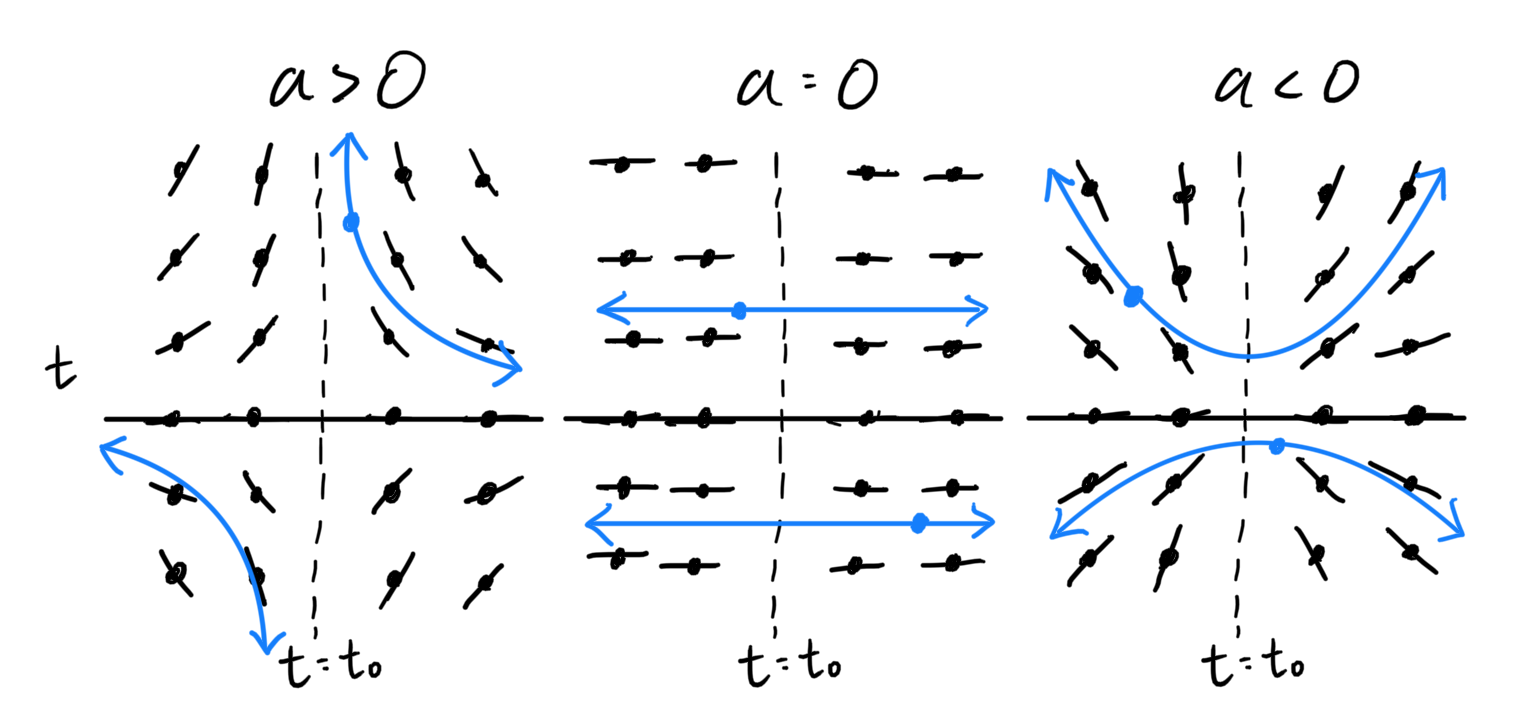
\includegraphics[scale=0.25]{img/Singular_Point_of_1st_Cauchy_Euler.PNG}
    \end{center}
    Given that $a > 0$, we can see that the solution is clearly unbounded at $t = t_0$, so there does not exist an analytic function. However, if $a \leq 0$, then there does exist an analytic function. 
    \end{example}

    \begin{example}[Nonexistence of Analytic Solutions in 2nd-Order Cauchy-Euler Equation]
    Consider the second-order Cauchy-Euler equation centered around $t = t_0$
    \[(t - t_0)^2 y^{\prime\prime} + (t - t_0) a_1 y^\prime + a_2 y = 0\]
    where $a_1, a_2$ are constants. Then, we can see that there cannot be analytic solutions to this DEQ at $t= t_0$ since the coefficients of the equivalent, normalized equation
    \[y^{\prime\prime} + \frac{a_1}{t - t_0} y^\prime + \frac{a_2}{(t-t_0)^2} y = 0\]
    are unbounded at $t = t_0$. However, in a neighborhood of any point $t_1 \neq t_0$, there does exist analytic solutions. Assuming $a_1 = a_2 = 1$, we can see that the solution $y = \varphi(t) = \cos(\ln{(t-t_0)}) + \sin(\ln{(t - t_0)})$ oscillates infinitely as $t \rightarrow t_0$. 
    \begin{center}
        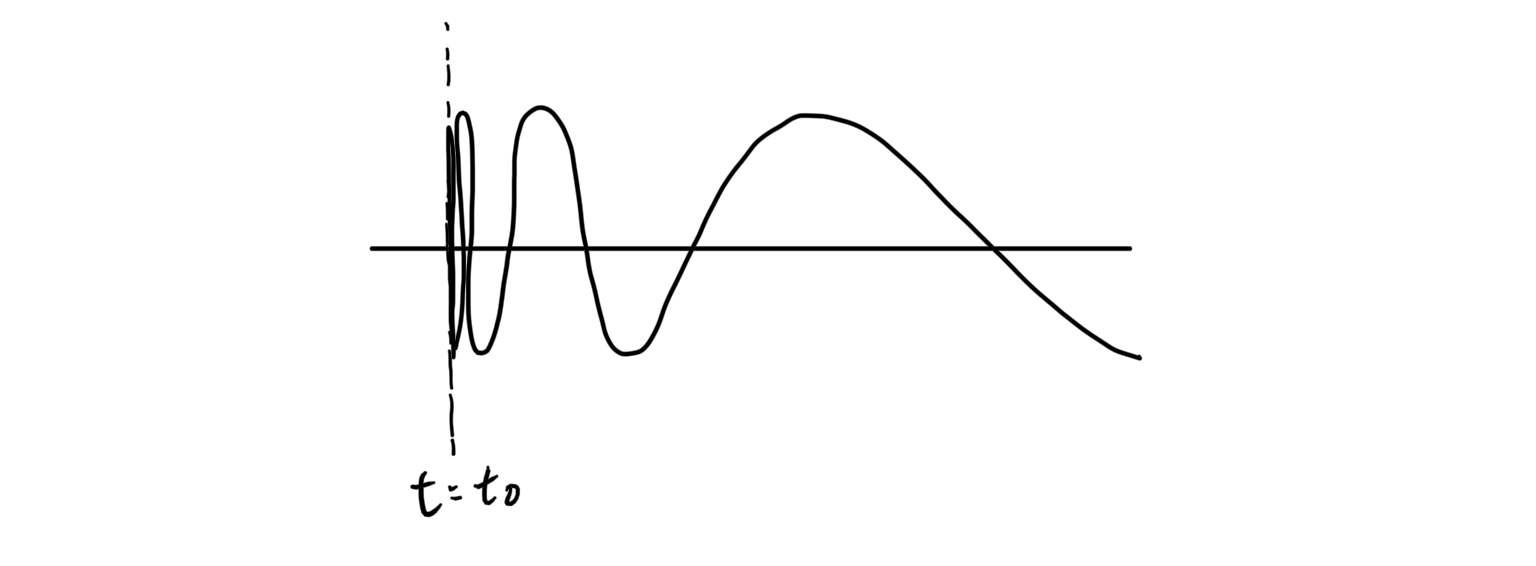
\includegraphics[scale=0.25]{img/Oscillates_Infinitely.PNG}
    \end{center}
    Furthermore, by setting this up as a system of first order equations using $y = y, x = y^\prime$, we get
    \begin{align*}
        y^\prime & = x \\
        x^{\prime} & = y^{\prime\prime} = - \frac{a_1}{t - t_0} x - \frac{a_2}{(t - t_0)^2} y
    \end{align*}
    Normalizing $a_1 = a_2 = 1$, we give the phase velocity vector field for the three time periods $t = t_0 - 1, t_0, t_0 + 1$. 
    \begin{center}
        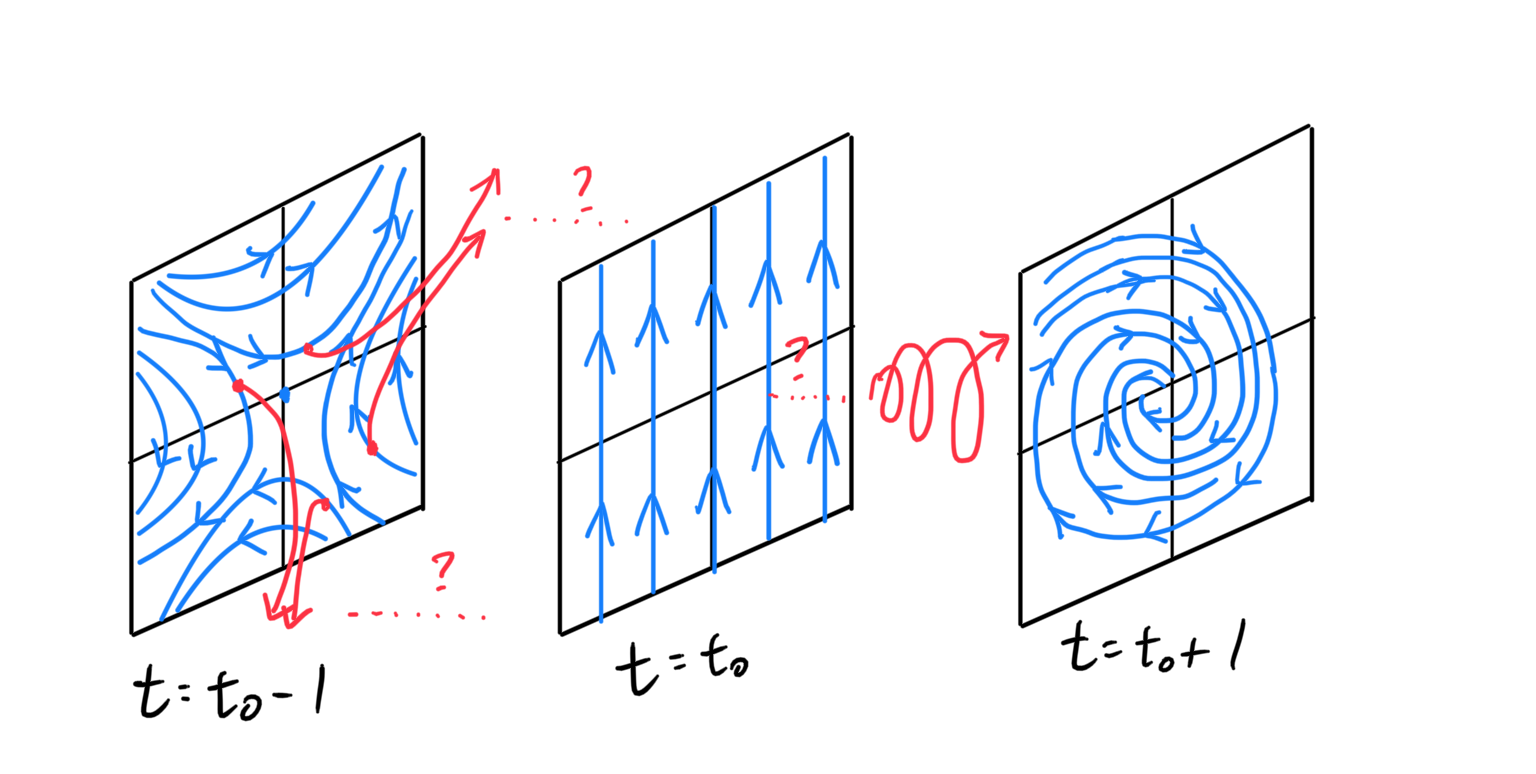
\includegraphics[scale=0.25]{img/Singular_Point_of_2nd_Cauchy_Euler.PNG}
    \end{center}
    \end{example}

    The behavior of the solutions near the singular point $t_0$ (whether it is actually analytic or not) depends on how rapidly $a_0 (t)$ approaches zero as $t \rightarrow t_0$. For this reason, we distinguish two different types of singular points, with the first being the regular one. 

    \begin{definition}[Regular Singular Point]
    The point $t_0$ is called a \textit{regular singular point} of the equation 
    \[\mathcal{L}_n (y) = a_0 (t) y^{(n)} + a_1 (t) y^{(n-1)} + \ldots + a_{n-1} (t) y^\prime + a_n (t) y = 0\]
    if it is a singular point and if 
    \[p_1 (t) = \frac{a_1 (t)}{a_0 (t)}, \; p_2 (t) = \frac{a_2 (t)}{a_0 (t)}, \ldots, p_n (t) = \frac{a_n (t)}{a_0 (t)}\]
    have the property that $(t - t_0) p_1 (t), (t - t_0)^2 p_2 (t), \ldots, (t - t_0)^n p_n (t)$ are all analytic at $t_0$. It immediately follows that the equation $\mathcal{L}_n (y) = 0$ has a regular singular point at $t = t_0$ if and only if it can be written in the form:
    \begin{align*}
        & a_0 (t) y^{(n)} + a_1 (t) y^{(n-1)} + \ldots + a_{n-1} (t) y^\prime + a_n (t) y = 0\\
        \implies & y^{(n)} + \frac{a_1 (t)}{a_0 (t)} y^{(n-1)} + \ldots + \frac{a_{n-1}}{a_0 (t)} (t) y^\prime + \frac{a_n (t)}{a_0 (t)} y = 0 \\
        \implies & (t - t_0)^n y^{(n)} + (t - t_0)^n \frac{a_1 (t)}{a_0 (t)} y^{(n-1)} + \ldots + (t - t_0)^n \frac{a_{n-1}}{a_0 (t)} (t) y^\prime + (t - t_0)^n \frac{a_n (t)}{a_0 (t)} y = 0 \\
        \implies & (t - t_0)^n y^{(n)} + (t - t_0)^{n-1} \bigg((t-t_0) \frac{a_1 (t)}{a_0 (t)}\bigg) y^{(n-1)} + \ldots + \bigg( (t-t_0)^n \frac{a_n (t)}{a_0 (t)} \bigg) y = 0 \\
        \implies & (t - t_0)^n y^{(n)} + (t - t_0)^{n-1} \alpha_1 (t) y^{(n-1)} + \ldots + (t - t_0) \alpha_{n-1} (t) y^\prime + \alpha_n (t) y = 0
    \end{align*}
    Therefore, the equation $\mathcal{L}_n (y) = 0$ has a regular singular point if it can be written in the form
    \[\sum_{i=0}^n (t - t_0)^{n-i} \alpha_i (t) y^{(n-i)} = 0, \;\;\;\; \alpha_i (t) = (t - t_0)^i \frac{a_i (t)}{a_0 (t)}\]
    where the $\alpha_i$'s are analytic at $t = t_0$. If a singular point $t = t_0$ is not regular, then it is called an \textit{irregular singular point}. 
    \end{definition}

    \begin{example}
    We list three examples of equations and their corresponding singular points. 
    \begin{enumerate}
        \item The Euler equation 
        \[(t - t_0)^2 y^{\prime\prime} + (t - t_0) a_1 y^\prime + a_2 y = 0\]
        is the simplest example of an equation which has a regular singular point at $t = t_0$. 
        \item The equation 
        \[t^2 y^{\prime\prime} + \frac{3}{2} t y^\prime + ty = 0\]
        has $t = 0$ as a regular singular point because $p(t) = \frac{3}{2t}, q(t) = \frac{1}{t}$ have the property that $t p(t) = \frac{3}{2}, t^2 q(t) = t$ are both analytic everywhere.
        \item The equation 
        \[(t-1)^3 y^{\prime\prime} + 2(t-1)^2 y^\prime - 7ty = 0\]
        does not have a regular singular point at $t = 1$. 
    \end{enumerate}
    \end{example}

    \subsubsection{Change of Basis}

      To simplify the process, we can perform a change of basis 
      \[t \mapsto x = t - t_0\]
      which allows us to transform the singular point $t_0$ to the origin without changing the form of the equation in any essential way. Therefore, we would let 
      \[\overline{\alpha}_i (x) = \alpha_i (t_0 + x) \text{ for all } i = 1, 2, \ldots, n\]
      which are analytic at $x = 0$ since $\alpha_i$ is analytic at $t = t_0$. Furthermore, we define
      \[\overline{y}(x) = y (t_0 + x)\]
      and by the chain rule, we have
      \[\frac{d \overline{y}}{dx} = y^\prime (t_0 + x) = y^\prime (t), \frac{d^2 \overline{y}}{dx^2} = y^{\prime\prime} (t_0 + x) = y^{\prime\prime} (t), \ldots, \frac{d^n \overline{y}}{dx} = y^{(n)} (t_0 + x) = y^{(n)} (t)\]
      Therefore, the equation simplifies as such: 
      \begin{align}
          & (t - t_0)^n y^{(n)} + (t - t_0)^{n-1} \alpha_1 (t) y^{(n-1)} + \ldots + (t - t_0) \alpha_{n-1} (t) y^\prime + \alpha_n (t) y = 0 \\
          \implies & x^n \bar{y}^{(n)}(x) + x^{n-1} \bar{\alpha}_1(x) \bar{y}^{(n-1)} (x) + \ldots + x \bar{\alpha}_{n-1} (x) \bar{y}^\prime (x) + \bar{\alpha}_n (x) \bar{y} = 0
      \end{align}
      Therefore, if $\bar{y}(x)$ is a solution of the second equation with regular singular point $x = 0$, then the function $y(t) = \bar{y} (t - t_0)$ is a solution of the first equation with regular singular point $t = t_0$. 

      Therefore, we will assume that such a preliminary simplification has been made, and without loss of generality, we will consider a $n$th order homogeneous linear differential equation with regular singular point (changed accordingly to be at $t = 0$) to be of form
      \[t^n y^{(n)} + t^{n-1} \alpha_1 (t) y^{(n-1)} + \ldots + t^2 \alpha_{n-2} (t) y^{\prime\prime} + t \alpha_{n-1} (t) y^\prime + \alpha_n (t) y = 0\]
      where the $\alpha_i$'s are given functions analytic at $t = 0$ and having power series expansions 
      \[\alpha_i (t) = \sum_{k=0}^\infty \alpha_{ik} t^k\]
      which converge in some interval $|t|<r$. 

    \subsubsection{Examples}

      \begin{example}
      The following DEQ can be changed as such
      \begin{align*}
          2ty^{\prime\prime} + y^\prime + ty & = 0 \implies t^2 y^{\prime\prime} + \frac{1}{2} ty^\prime + \frac{1}{2} t^2 y = 0 \\
          & = t^2 y^{\prime\prime} + t \alpha_1 (t) y^\prime + \alpha_2 (t) y = 0
      \end{align*}
      where
      \[\alpha_1 (t) = \frac{1}{2}, \;\; \alpha_2 (t) = \frac{1}{2} t^2\]
      which are both analytic at $t = 0$, making $t = 0$ a regular singular point. If both $\alpha_1, \alpha_2$ were constants, this following equation would be the Euler equation, making one of the solutions to be of form $|t|^z$. But since $\alpha_2$ is not a constant, we attempt to find a solution of form 
      \[|t|^z \sum_{k=0}^\infty c_k t^k, \;\;\; c_0 \neq 0\]
      where the constants $z, c_k$ are determined by substitution into the differential equation within some interval of convergence around $t = 0$. Since $t = 0$ is a singular point, we separate the cases $t>0$ and $t<0$. We first consider the case $t>0$ and try the following solution of $\varphi$ and its derivatives (assuming $\varphi \in C^2$): 
      \begin{align*}
          \varphi (t) & = t^z \sum_{k=0}^\infty c_k t^k = \sum_{k=0}^\infty c_k t^{z+k} \\
          \varphi^\prime (t) & = \sum_{k=0}^\infty c_k (z+k) t^{z+k-1} \\
          \varphi^{\prime\prime} (t) & = \sum_{k=0}^\infty c_k (z+k)(z+k-1) t^{z+k-2} 
      \end{align*}
      We substitute this into the equation and simplify it, where we set the indicial polynomial as $f(z) = z (z - \frac{1}{2})$ (we can find this by looking at the quadratic term in $z$ having coefficient $c_0$). 
      \begin{align*}
          0 & = t^2 \varphi^{\prime\prime} (t) + \frac{1}{2} t \varphi^\prime (t) + \frac{1}{2} t^2 \varphi (t) \\
          & = c_0 z \bigg(z - \frac{1}{2}\bigg) t^z + c_1 (z+1) \bigg( z+\frac{1}{2}\bigg) t^{z+1} + \sum_{k=0}^\infty \bigg( (z+k) \Big(z+k-\frac{1}{2} \Big) c_k + \frac{1}{2} c_{k-2}\bigg) t^{z+k}\\
          & = t^z \Bigg( c_0 f(z) + c_1 f(z+1) t + \sum_{k=2}^\infty \bigg( f(z+k) c_k + \frac{1}{2} c_{k-2} \bigg)\Bigg) 
      \end{align*}
      The equality implies that every coefficient of every power of $t$ vanishes on the right hand side. Since we assumed $c_0 \neq 0$, we have
      \begin{align*}
          &f(z) = 0 \\
          &c_1 f(z+1) = 0 \\
          &f(z+k) c_k + \frac{1}{2} c_{k-2} = 0 \text{ for } k = 2, 3, 4, \ldots 
      \end{align*}
      $f(z) = 0 \implies z = 0$ or $z = \frac{1}{2}$. 
      \begin{enumerate}
          \item When $z = \frac{1}{2}$, this must mean that $c_1 = 0$ in order to satisfy the equation $c_1 f(z+1) = 0$. We can rewrite the relation $f(z+k) c_k + \frac{1}{2} c_{k-2} = 0$ as
          \[c_k = \frac{-1}{2 f(k + \frac{1}{2})} c_{k-2} = -\frac{1}{2k (k+\frac{1}{2})} c_{k-2}\]
          Remember that $c_0 \neq 0$ is arbitrary and that $c_1 = 0$, so we can manually calculate 
          \begin{align*}
              c_{2m-1} & = 0 \\
              c_{2m} & = (-1)^m \frac{c_0}{2 \cdot 4 \cdot 6 \ldots 2m \cdot 5 \cdot 9 \ldots (4m+1)} = (-1)^m c_0 \bigg( \prod_{i=1}^m 2i (4i + 1) \bigg)^{-1}
          \end{align*}
          for $m = 1, 2, \ldots $. Substituting these quantities into the series $\varphi(t) = t^z \sum_{k=0}^\infty c_k t^k$ gives
          one candidate for a solution of the differential equation for $t>0$:
          \[\varphi_1 (t) = t^{1/2} \Bigg( 1 + \sum_{m=1}^\infty (-1)^m \bigg( \prod_{i=1}^m 2i (4i + 1) \bigg)^{-1} t^{2m} \Bigg) \]
          Note that the $c_0$, which is just a constant factor, has been normalized to $1$. 
          \item When $z = 0$, we find that $c_1 = 0$ ($c_0$ still arbitrary), but we rewrite the relation $f(z+k) c_k + \frac{1}{2} c_{k-2} = 0$ as 
          \[c_k = \frac{-1}{2 f(k)} c_{k-2} = -\frac{1}{2k (k-\frac{1}{2})} c_{k-2}\]
          Leading to
          \begin{align*}
              c_{2m-1} & = 0 \\
              c_{2m} & = (-1)^m \frac{c_0}{2 \cdot 4 \cdot 6 \ldots 2m \cdot 3 \cdot 7 \ldots (4m-1)} = (-1)^m c_0 \bigg( \prod_{i=1}^m 2i (4i - 1) \bigg)^{-1}
          \end{align*}
          for $m = 1, 2, \ldots $. Substituting and normalizing $c_0 = 1$, we obtain the second candidate for a solution of the DEQ when $t>0$ as
          \[\varphi_2 (t) = 1 + \sum_{m=1}^\infty (-1)^m \bigg( \prod_{i=1}^m 2i (4i - 1) \bigg)^{-1} t^{2m}\]
      \end{enumerate}
      Using the ratio test, we can find out that for the series $\varphi_1, \varphi_2$, 
      \[\bigg|\frac{a_{m+1}}{a_{m}}\bigg| \rightarrow 0 \text{ as } m \rightarrow \infty\]
      where $a_m$ is the $m$th term of the series. Therefore, both $\varphi_1, \varphi_2$ converges within $(-\infty, \infty)$. Therefore, we have found solutions of the form 
      \[|t|^z \sum_{k=0}^\infty c_k t^k\]
      for when $t>0$ (the value $t=0$ must be omitted because the differential equation has no meaning at the singular point $t=0$). It is easy to prove that $\varphi_1$ and $\varphi_2$ are linearly independent. The above calculations are all valid for $t<0$ if $t^z$ is replaced by $|t|^z = e^{z \log{|t|}}$, and still leads to the same solutions $\varphi_1, \varphi_2$ for the interval $(-\infty, 0)$.
      \end{example}

      Therefore, we can see that the assumption that a given DEQ has a solution of the form 
      \[|t|^z \sum_{k=0}^\infty c_k t^k\]
      leads to a quadratic equation in $z$, the indicial equation, and each root of the indicial equation leads to two linearly independent solutions of the differential equation. However, an indicial polynomial may have a double root, which will require extra work to find the second solution. 

      \begin{example}
      The differential equation $t y^{\prime\prime} + y^\prime + y = 0$, which may be written as 
      \[t^2 y^{\prime\prime} + t y^\prime + ty = 0\]
      Clearly, $t=0$ is a regular singular point. Assuming the existence of solution of the form $\varphi(t) = |t|^z \sum_{k=0}^\infty c_k t^k$ on some interval, we consider the case $t>0$. With some steps omitted, we have
      \[t^2 \varphi^{\prime\prime} (t) + t \varphi^\prime (t) + t \varphi(t) = t^z \bigg( f(z) c_0 + \sum_{k=1}^\infty \big( f(k+z) c_k + c_{k-1} \big) t^k \bigg)\]
      where the indicial polynomial is $f(z) = z^2$, having a double root $z=0$. Since every term on the right hand side vanishes, we have
      \begin{align*}
          f(k+z) c_k + c_{k-1} = 0 & \implies c_k = -\frac{c_{k-1}}{k^2}, \;\;\;\; k = 1, 2, 3, \ldots \\
          & \implies c_k = c_0 \prod_{i=1}^k -\frac{1}{i^2}
      \end{align*}
      By substituting in the $c_k$'s, we have (for $t>0$)
      \[\varphi(t) = 1 + t^z \sum_{k=1}^\infty \bigg(\prod_{i=1}^k -\frac{1}{i^2}\bigg) t^k\]
      Similar calculations show that the same solution pops up for $t<0$. The ratio test tells us that the interval of convergence for $\varphi(t)$ is $(-\infty, \infty)$. We will talk about how to find the second solution later. 
      \end{example}

      Note in the previous example that although the differential equation makes no sense at the singular point $t = 0$, the function defined by the series 
      \[\sum_{k=0}^\infty c_k t^k\]
      is well defined 

      \begin{example}
      The DEQ $t y^{\prime\prime} + ty^\prime - y = 0$, which can be rewritten as
      \[t^2 y^{\prime\prime} + t^2 y^\prime - ty = 0\]
      has $t = 0$ has a regular singular point. When $t>0$, we calculate
      \[^2 y^{\prime\prime} + t^2 y^\prime - ty =  = t^z \bigg( f(z) c_0 + \sum_{k=1}^\infty \big( f(k+z) c_k + (k+z-2) c_{k-1}\big) t^k \bigg)\]
      where $f(z) = z (z-1)$. For every term to vanish, $z = 0$ or $z = 1$. 
      \begin{enumerate}
          \item Taking $z = 1$, we have 
          \[c_k = -\frac{(k-1) c_{k-1}}{k (k+1)}, \;\; k = 1, 2, \ldots\]
          which gives $c_k = 0$ and taking $c_0 = 1$, have have solution $\varphi_1 (t) = |t|$, which is clearly convergent. 
          \item When $z=0$, the recursion formula becomes
          \[k(k-1) c_k + (k-2) c_{k-1} = 0, \;\; k = 1, 2, \ldots\]
          But taking $k=1$, $c_1$ must be determined from the relation 
          \[0 \cdot c_1 - c_0 = 0\]
          But since $c_0 \neq 0$, this is impossible and there can be no solution of the assumed form corresponding to the root $z=0$. However, a solution of a different form does exist. 
      \end{enumerate}
      \end{example}

    \subsubsection{Regular Singular Point Theorem}

      We can neatly summarize our theory of finding solutions of equation with singular points with the following theorem. 

      \begin{theorem}[Regular Singular Point Theorem of 2nd-Order Homogeneous Linear DEQs]
      Consider the differential equation
      \[t^2 y^{\prime\prime} + t \alpha_1 (t) y^\prime + \beta (t) y = 0\]
      where $\alpha_1, \beta$ are analytic at regular singular point $t = 0$ and have expansions
      \[\alpha (t) = \sum_{k=0}^\infty \alpha_k t^k, \;\;\; \beta(t) = \sum_{k=0}^\infty \beta_k t^k\]
      which converge for $|t|<r$ for some $r>0$. Let $z_1, z_2$ be the roots of the indicial equation
      \[f(z) = z(z-1) + \alpha_0 z + \beta_0 = 0\]
      with Re$(z_1) \geq$ Re$(z_2)$. Then, there is always a solution of the form 
      \[\varphi_1 (t) = |t|^{z_1} \sum_{k=0}^\infty c_k t^k \;\;\;\;\; (c_0 = 1)\]
      in the punctured interval $0<|t|<r$ whose coefficients $c_k$ can be determined recursively from the equations
      \[f(z_1 + k) c_k = - \sum_{j=0}^{k-1} \big((j+z)\alpha_{k-j} + \beta_{k-j}\big) c_j, \;\;\;\;\; k = 1, 2, \ldots\]
      As for the second solution, there are three possible cases: 
      \begin{enumerate}
          \item If $z_1 \neq z_2, z_1 - z_2 \not\in \mathbb{Z}$, then there is a second, linearly independent solution of the form 
          \[\varphi_2 (t) = |t|^{z_2} \sum_{k=0}^\infty \hat{c}_k t^k \;\;\;\;\; (\hat{c}_0 = 1)\]
          also in the punctured interval $0 < |t| < r$. The coefficients $\hat{c}_k$ can also be solved using the recursive formula above, with $z_1$ replaced by $z_2$ and $c_k$ replaced by $\hat{c}_k$. 
          \item If $z_1 = z_2$, then the second (linearly independent) solution is of form
          \[\varphi_2 (t) = |t|^{z_1 + 1} \bigg( \sum_{k=0}^\infty b_k t^k\bigg) + \varphi_1 (t) \log{|t|}\]
          valid for $0<|t|<r$, whose coefficients $b_k$ can be determined by direct substitution into the DEQ. 
          \item If $z_1 - z_2 \in \mathbb{N}$, then there is a second linearly independent solution of form 
          \[\varphi_2 (t) = |t|^{z_2} \bigg( \sum_{k=0}^\infty b_k t^k \bigg) + a \varphi_1 (t) \log{|t|}\]
          valid for $0<|t|<r$, where $a$ is a constant (possibly $0$) and the coefficients $b_k$ can be determined by direct substitution into the DEQ. 
      \end{enumerate}
      \end{theorem}

      Note that it is simpler in practice to substitute the assumed formula of the solution into the DEQ than to use the recursive formulas to solve for the coefficients. 

    \subsubsection{The Bessel Equation}

      \begin{definition}[Bessel Equation]
      The \textbf{Bessel equation} arises in a natural way in many mathematical physics problems having axial/cylindrical symmetry, and is written in the form 
      \[\mathcal{L}_n (y) = t^2 y^{\prime\prime} + t y^\prime + (t^2 - p^2) y = 0\]
      where constant $p \in \mathbb{C}$ and Re$(p) \geq 0$. The point $t = 0$ is a regular singular point, and the equation is of form $t^2 y^{\prime\prime} + t \alpha(t) y^\prime + \beta(t) y = 0$. 
      \end{definition}

      \begin{definition}
      Recall the gamma function
      \[\Gamma (z) = \int_0^\infty e^{-x} x^{z-1} \,dx, \;\;\;\;\; \text{Re}(z) > 0\]
      and its properties: 
      \begin{enumerate}
          \item $\Gamma(z)$ is well defined and continuous for Re$(z) > 0$. 
          \item $\Gamma(1) = 1, \Gamma(\frac{1}{2}) = \sqrt{\pi}$
          \item $\Gamma(z) = (z-1) \Gamma (z-1)$ for Re$(z) > 1$ from integration by parts. 
          \item $\Gamma(z) = z!$ for $z \in \mathbb{N}$. 
          \item We can define $\Gamma$ for negative non-integer numbers $z$ using the recursion formula 
          \[\Gamma(z) = \frac{\Gamma(z+k)}{z (z+1) \ldots (z+k-1)}\]
          by choosing a positive integer $k$ such that Re$(z+k)>0$. Therefore, we can define $\Gamma$ for all complex numbers $z$ except for when Re$(z) \in \{0, -1, -2, -3, \ldots\}$. The graph of $\Gamma$ in $\mathbb{R} \times \mathbb{R}$ is shown. 
          \begin{center}
              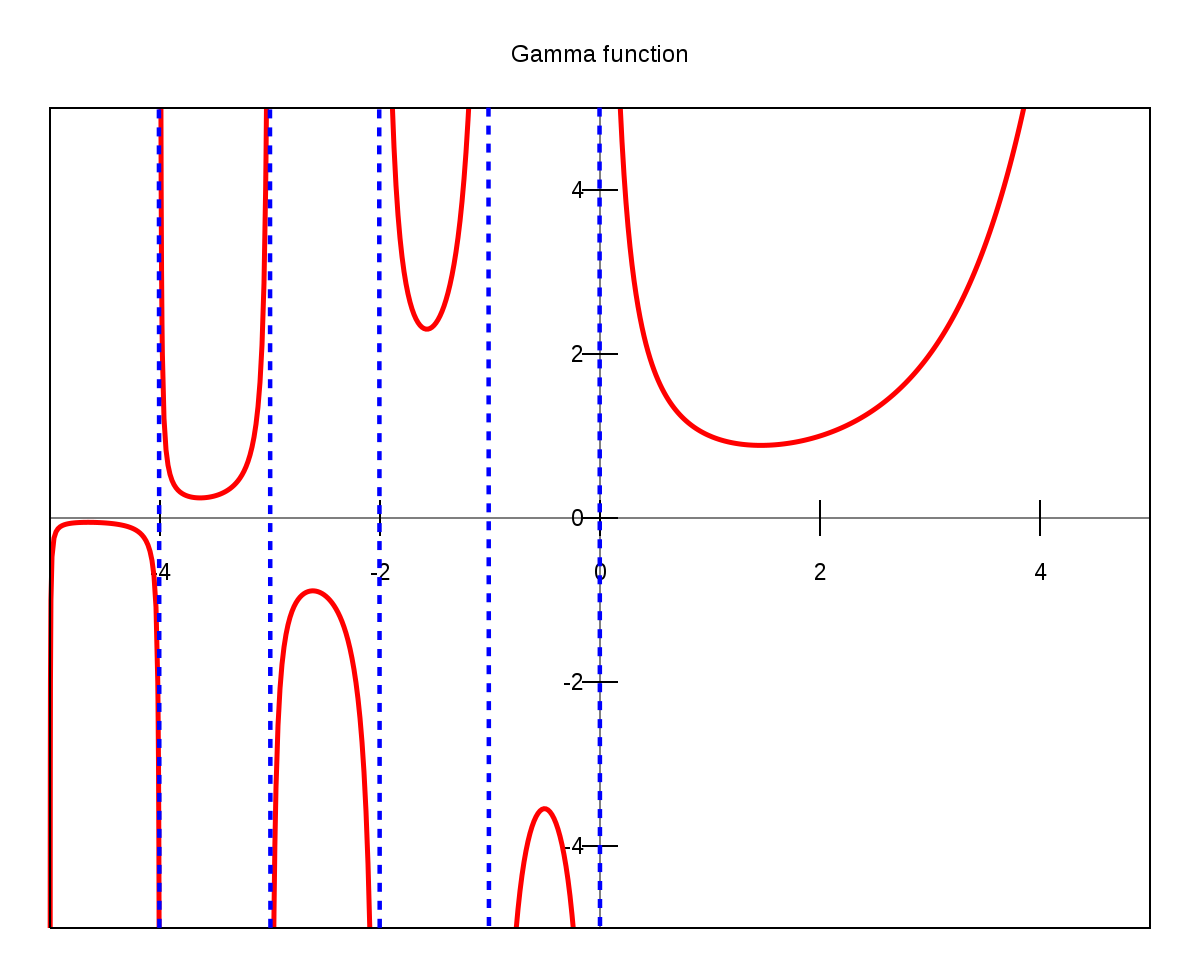
\includegraphics[scale=0.25]{img/Gamma_plot.png}
          \end{center}
      \end{enumerate}
      \end{definition}

      \begin{theorem}[The Bessel Function]
      Given the Bessel equation 
      \[t^2 y^{\prime\prime} + t y^\prime + (t^2 - p^2) y = 0, \;\; p \in \mathbb{C}, \text{Re}(p) \geq 0\]
      where $t = 0$ is a regular singular point. 
      \begin{enumerate}
          \item If $p \not\in \mathbb{N} \cup \{0\}$, then the following \textit{Bessel functions of the first kind} $J$ (of index $p, -p$) 
          \begin{align*}
              J_p (t) & = \bigg| \frac{t}{2}\bigg|^p \sum_{m=0}^\infty \frac{(-1)^m}{m! \Gamma(p+m+1)} \bigg(\frac{t}{2}\bigg)^{2m} \\
              J_{-p} (t) & = \bigg| \frac{t}{2}\bigg|^{-p} \sum_{m=0}^\infty \frac{(-1)^m}{m! \Gamma(m-p+1)} \bigg(\frac{t}{2}\bigg)^{2m}
          \end{align*}
          are two linearly independent solutions for $0 < |t| < \infty$. 
          \item If $p = 0$, then the Bessel function of the first kind and second kind, both of index $0$
          \begin{align*}
              J_0 (t) & = \sum_{m=0}^\infty \frac{(-1)^m}{(m!)^2} \bigg( \frac{t}{2}\bigg)^{2m} \\
              K_0 (t) & = - \sum_{m=1}^\infty \Bigg( \frac{(-1)^m}{(m!)^2} \bigg(1 + \frac{1}{2} + \ldots + \frac{1}{m} \bigg) \bigg(\frac{t}{2}\bigg)^{2m} \Bigg) + J_0 (t) \log{t}
          \end{align*}
          are two linearly independent solutions for $0 < |t|<\infty$. 
          \item If $p$ is a positive integer $n$, then the Bessel function of the first kind of index $n$ and the \textit{Bessel function of the second kind} $K$ (of index n)
          \begin{align*}
              J_n (t) & = \bigg| \frac{t}{2}\bigg|^n \sum_{m=0}^\infty \frac{(-1)^m}{m! \Gamma(n+m+1)} \bigg(\frac{t}{2}\bigg)^{2m} \\
              K_n (t) & = -\frac{1}{2} \bigg|\frac{t}{2}\bigg|^{-n} \bigg(\sum_{k=0}^{n-1} \frac{(n-k-1)!}{k!} \bigg(\frac{t}{2}\bigg)^{2k} + \frac{1}{n!}\bigg(1 + \frac{1}{2} + \ldots + \frac{1}{n}\bigg)\bigg(\frac{t}{2}\bigg)^{2n} \Bigg) \\
              & -\frac{1}{2} \bigg(\frac{t}{2} \bigg)^n \sum_{k=0}^\infty \frac{(-1)^k}{k!(k+n)!} \bigg(\Big(1 + \ldots + \frac{1}{k}\Big) + \Big(1 + \frac{1}{2} + \ldots + \frac{1}{k+n}\Big) \bigg) \bigg(\frac{t}{2}\bigg)^{2k} \\
              & + J_n (t) \log{|t|}
          \end{align*}
      \end{enumerate}
      \end{theorem}
      \begin{proof}
      We now derive the solutions to this Bessel equation. By the regular singular point theorem, since
      \[\alpha (t) = 1, \;\; \beta(t) = -p^2 + t^2\]
      which both converge for $|t|<\infty$, the indicial equation is 
      \[f(z) = z(z-1) + z + -p^2 = z^2 - p^2\]
      which has zeroes $z_1 = p, z_2 = -p$ (remember we assumed (Re$(p) \geq 0$). If $p \neq 0$ and if $z_1 - z_2 = 2p$ is not a positive integer (i.e. $p$ is not $0$, an integer, or a half-integer), there exists two linearly independent solutions $\varphi_1, \varphi_2$ of the equation, valid for $0<|t|<\infty$, of the form
      \begin{align*}
          \varphi_1 (t) & = |t|^p \sum_{k=0}^\infty c_k t^k \;\;\;\;\; (c_0 \neq 0) \\
          \varphi_2 (t) & = |t|^{-p} \sum_{k=0}^\infty \hat{c}_k t^k \;\;\;\; (\hat{c}_0 \neq 0)
      \end{align*}
      where coefficients $c_k, \hat{c}_k$ are determined recursively by substitution. We first compute $\varphi_1$ and assume $t>0$. Substituting
      \[\varphi_1^\prime (t) = \sum_{k=0}^\infty c_k (p+k) t^{p+k-1}, \;\;\; \varphi_1^{\prime\prime} = \sum_{k=0}^\infty c_k (p+k) (p+k-1) t^{p+k-2}\]
      into the equation and simplifying gives
      \[\mathcal{L}_2 \big( \varphi_1 (t)\big) = t^p \bigg( f(p) c_0 + f(p+1) c_1 t + \sum_{k=0}^\infty \big( f(p+k) c_k + c_{k-2}\big) t^k \bigg) = 0\]
      for which we conclude that 
      \[f(p+1) c_1 = 2p + 1 = 0 \implies p = -\frac{1}{2} \text{ or } c_1 = 0\]
      But since Re$(p)\geq 0$, this means that $c_1 = 0$. We use the recursive relations
      \[f(p+k) c_k + c_{k-2} = k (2p+k) c_k + c_{k-2} = 0\]
      which implies that
      \begin{align*}
          c_{2m-1} & = 0 \\
          c_{2m} & = \frac{(-1)^m c_0}{2^{2m} m! (p+1)(p+2) \ldots (p+m)} 
      \end{align*}
      for $m = 1, 2, \ldots$. Therefore, the solution can be written as
      \[\varphi_1 (t) = c_0 |t|^p \Bigg( 1 + \sum_{m=1}^\infty \frac{(-1)^m t^{2m}}{2^{2m} m! (p+1) (p+2) \ldots (p+m)} \Bigg)\]
      Since we can let $c_0$ be any nonzero constant, we define it using the Gamma function as
      \[c_0 = \frac{1}{2^p \Gamma(p+1)}\]
      resulting in the solution
      \[J_p = \bigg| \frac{t}{2}\bigg|^p \sum_{m=0}^\infty \frac{(-1)^m}{m! \Gamma(p+m+1)} \bigg(\frac{t}{2}\bigg)^{2m}\]
      called the \textit{Bessel function of the first kind of index $p$}. It is well defined for all $t \in \mathbb{R}$ and satisfies the DEQ for $0 < |t| < \infty$. 
      \end{proof}

    \subsubsection{Singularities at Infinity}

      We can also study the behavior of solutions of the equation
      \[\mathcal{L}_2 (y) = y^{\prime\prime} + p(t) y^\prime + q(t) y = 0\]
      as $|t| \rightarrow \infty$ by making the change of variable $t = 1/x$ and studying the behavior of solutions of the resulting equation as $x \rightarrow 0$. Thus, we let $\varphi$ be a solution of the original DEQ for $|t|>R$ and let
      \[\psi(x) = \varphi(\frac{1}{x}), \;\; \bar{p}(x) = p(\frac{1}{x}), \;\; \bar{q}(x) = q(\frac{1}{x})\]
      which should all be well-defined for $|x|<1/R$. By the chain rule, we have
      \begin{align*}
          \varphi^\prime (t) & = -\frac{1}{t^2} \psi^\prime (x) = -x^2 \psi^\prime (x) \\
          \varphi^{\prime\prime} (t) & = \frac{1}{t^4} \psi^{\prime\prime} (x) + \frac{2}{t^3} \psi^\prime (x) = x^4 \psi^{\prime\prime}(x) + 2x^3 \psi^\prime (x) 
      \end{align*}
      Substituting this in shows that $\psi$ satisfies the new equation
      \[\bar{\mathcal{L}}_2 (z) = x^4 z^{\prime\prime} + \big( 2x^3 - x^2 \bar{p}(x)\big) z^\prime + \bar{q} (x) z= 0\]
      in which $x$ is the independent variable and $z$ is the function. Therefore, if $\psi$ satisfies $\bar{\mathcal{L}}_2 (z) = 0$ and if $\varphi(t) = \psi(1/t)$, then $\varphi$ satisfies $\mathcal{L}_2 (y) = 0$. Our results lead to the following theorem. 

      \begin{theorem}[Singularities at Infinity]
      $\infty$ is an ordinary point, a regular singular point, or an irregular singular point for the equation $\mathcal{L}_2 (y) = 0$ if and only if $0$ is respectively an ordinary point, a regular singular point, or an irregular singular point for the equation $\bar{\mathcal{L}}_2 (z) = 0$. 
      \end{theorem}

      \begin{example}
      Given the equation
      \[y^{\prime\prime} + a y^\prime + by = 0, \;\;\;\;\; a, b \in \mathbb{R}\]
      The change of variable $t = 1/x$ transforms this equation to
      \[x^4 z^{\prime\prime} + (2x^3 - ax^2) z^\prime + bz = 0\]
      which has an irregular singular point at $x = 0$. Therefore, the original equation has an irregular singular point at $t = \infty$. 
      \end{example}

\section{Systems of DEQs}

  \subsection{First-Order Systems}

    We expand on the theory of solving first order differential equations by studying systems of them, which can be worked on using vector algebra/calculus. 

    \begin{definition}[System of 1st Order Equations]
    A system of $n$ first order equations can be put in the form 
    \[y^\prime = f(t, y) \begin{cases}
    y_1^\prime  = f_1 (t, y_1, y_2, \ldots, y_n) \\
    y_2^\prime  = f_2 (t, y_1, y_2, \ldots, y_n) \\
    \ldots \\
    y_n^\prime  = f_n (t, y_1, y_2, \ldots, y_n) 
    \end{cases}\]
    where $f: D \subset \mathbb{R} \times \mathbb{R}^n \longrightarrow \mathbb{R}^n$ is defined in some $(n+1)$-dimensional region $D$ ($\mathbb{R}$ being the time continuum and $\mathbb{R}^n$ being the $n$-dimensional phase space). That is, at a certain time $t = t_0$, 
    \[f(t_0, \cdot): \mathbb{R}^n \longrightarrow \mathbb{R}^n\]
    determines the phase velocity vector field of $\mathbb{R}^n$ for that instance of time. If the system is autonomous, then the vector field does not morph. As shown before, we can visualize the following. 
    \begin{enumerate}
        \item System with 1-dimensional phase space (i.e. a system of one equation) 
        \begin{center}
            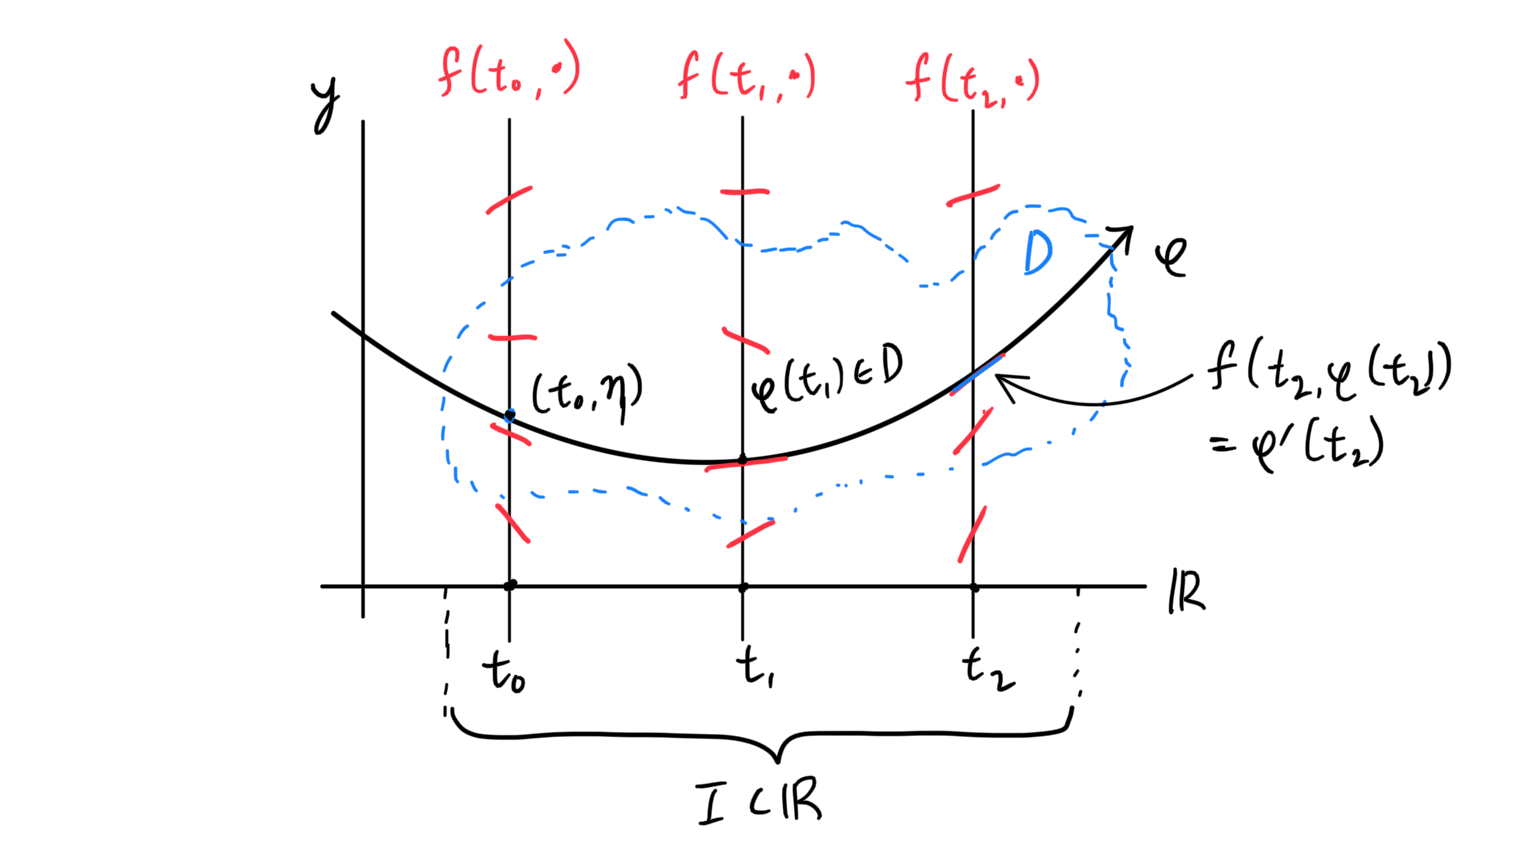
\includegraphics[scale=0.26]{img/System_w_1_dim_Phase_Space.PNG}
        \end{center}
        \item System with 2-dimensional phase space (two equations). The solution shown is 
        \[\varphi: \mathbb{R} \longrightarrow \mathbb{R}^2, \;\; y = \varphi(t) \iff \begin{pmatrix}y_1 \\ y_2
        \end{pmatrix} = \begin{pmatrix} \varphi_1 \\ \varphi_2 \end{pmatrix} (t) = \begin{pmatrix} \varphi_1 (t) \\ \varphi_2 (t) \end{pmatrix}\]
         \begin{center}
            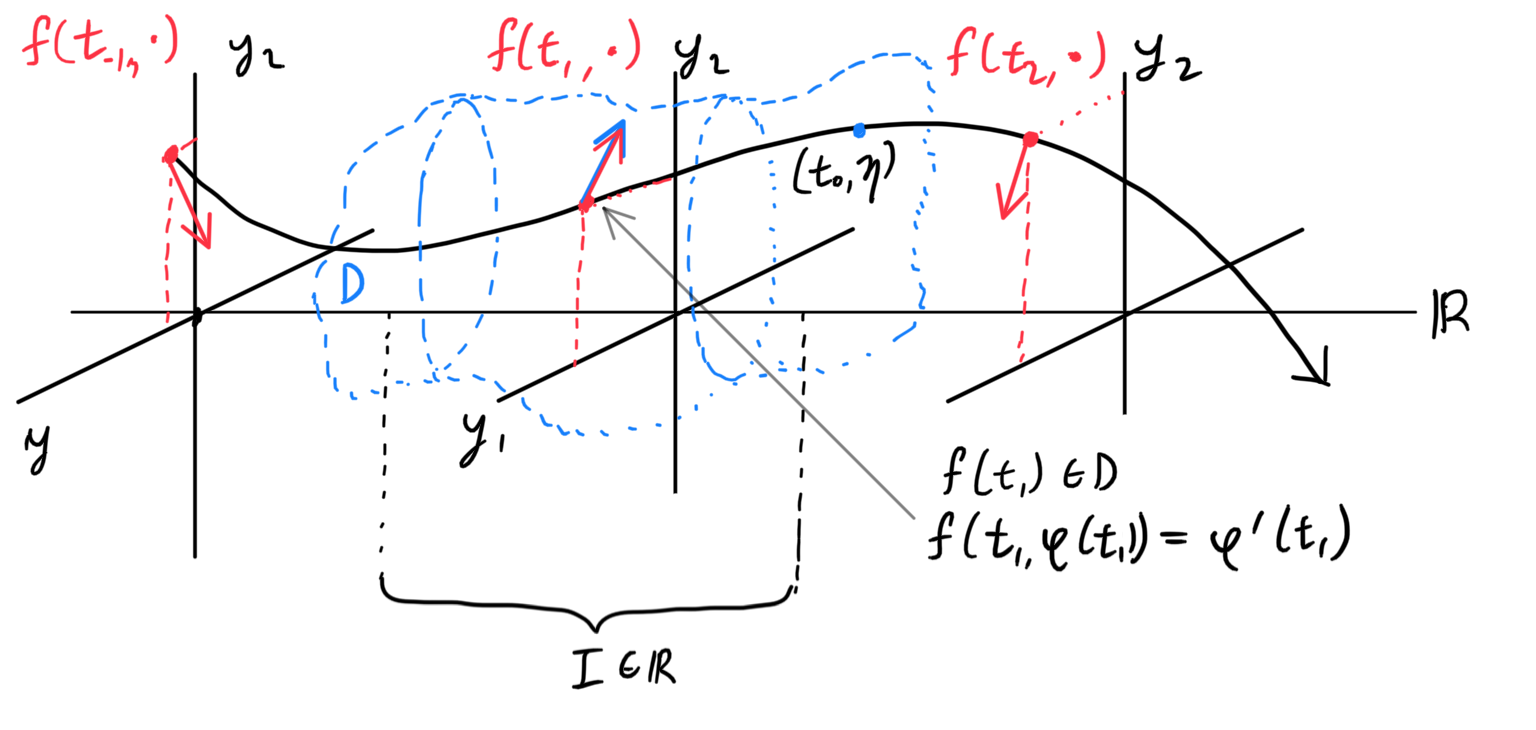
\includegraphics[scale=0.26]{img/System_w_2_dim_Phase_Space.PNG}
        \end{center}
        \item Systems with higher-dimensional phase spaces are harder to visualize, but we just imagine a time continuum $\mathbb{R}$ where at each point $t_0 \in \mathbb{R}$, there is a vector space $\mathbb{R}^n$ with a vector field $f(t_0, \cdot): \mathbb{R}^n \longrightarrow \mathbb{R}^n$ associated with it. In the visual below, the phase space are shown to be $\mathbb{R}^3$ (when it is really $\mathbb{R}^n$), with $D$ being represented by its cross sections in the time axis (e.g. $D_{t_0}$ is the cross section of $D$ at $t=t_0$). The solution curve $\varphi$ isn't explicitly shown (only the points on the curve at times $t=t_0, t_1, t_2$), but it would be of form 
        \[\varphi: \mathbb{R} \longrightarrow \mathbb{R}^3, y = \varphi(t) \iff \begin{pmatrix}
        y_1 \\ y_2 \\ y_3 \end{pmatrix} = \begin{pmatrix}
        \varphi_1 \\ \varphi_2 \\ \varphi_3 \end{pmatrix} (t) = \begin{pmatrix}
        \varphi_1 (t)\\ \varphi_2(t) \\ \varphi_3(t) \end{pmatrix}\]
         \begin{center}
            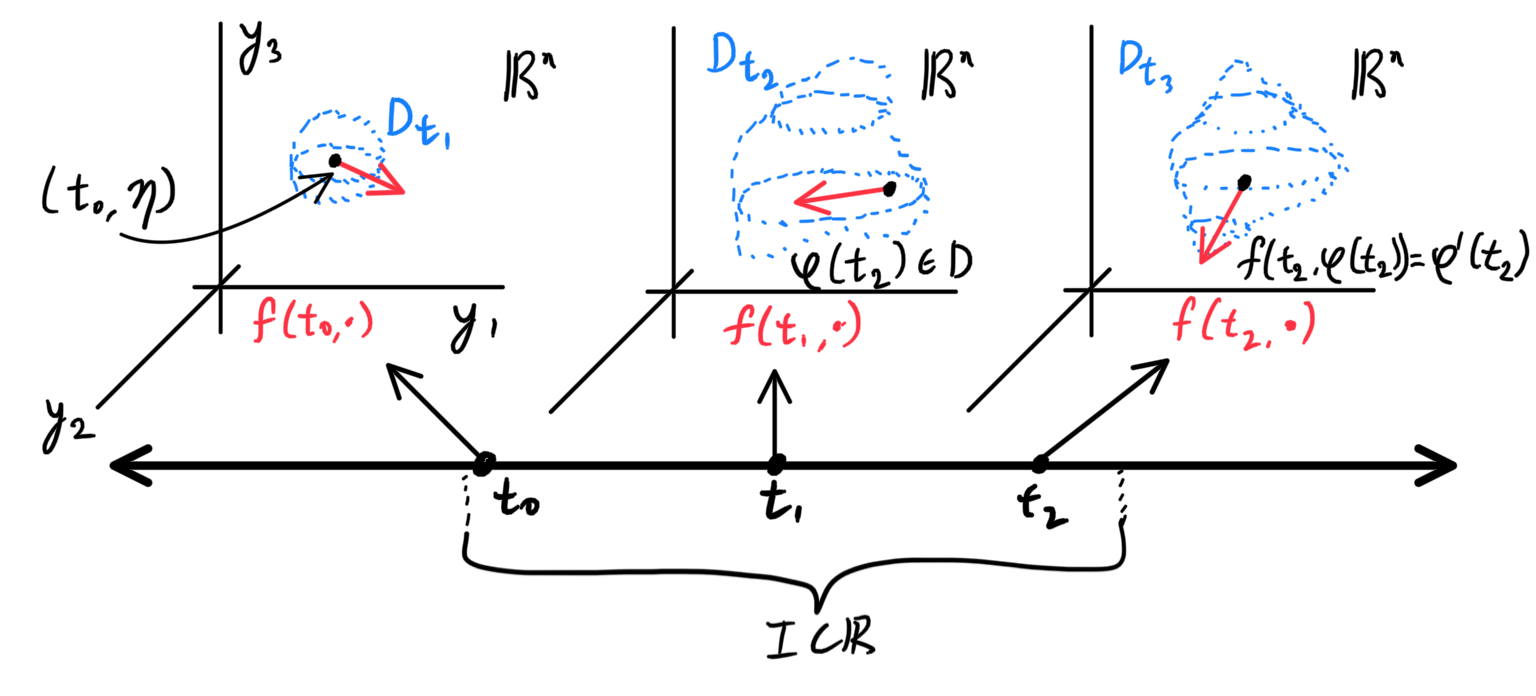
\includegraphics[scale=0.26]{img/System_w_n_dim_Phase_Space.PNG}
        \end{center}
    \end{enumerate}
    To find the solution of the system means to find the $n$ equations $y_1 = \varphi_1 (t), y_2 = \varphi_2 (t), \ldots, y_n = \varphi_n (t)$, which is equivalent to finding the vector-valued path function 
    \[y = \varphi(t) = \begin{pmatrix} \varphi_1 (t) \\ \vdots \\ \varphi_n (t) \end{pmatrix}, \varphi: I \subset \mathbb{R} \longrightarrow \mathbb{R}^n\]
    such that
    \begin{enumerate}
        \item the point $\big(t, \varphi(t)\big) \in D$ for each $t \in I$
        \item $\varphi^\prime (t)$ exists for each $t \in I$
        \item $\varphi^\prime (t) = f \big( t, \varphi(t)\big)$ for every $t \in I$ 
    \end{enumerate}
    To solve an initial value problem for the system with initial condition 
    \[\varphi(t_0) = \eta, \;\;\; \eta \in \mathbb{R}^n \text{ and } (t_0, \eta) \in D\]
    means to find a solution $\varphi$ of the system such that $\varphi(t_0) = \eta$. 
    \end{definition}

    The study of first order equations is quite nice because we can reduce a high-order scalar differential equation of form
    \[y^{(n)} = g(t, y, y^\prime, \ldots, y^{(n-1)})\]
    to the following system with a change of variable $y_1 = y, y_2 = y^\prime, \ldots, y_n = y^{(n-1)}$. 
    \[\begin{pmatrix}
    y_1 \\ y_2 \\ \vdots \\ y_{n-1} \\ y_n
    \end{pmatrix}^\prime = \begin{pmatrix}
    y_2 \\ y_3 \\ \vdots \\ y_n \\ g(t, y_1, y_2, \ldots, y_n)
    \end{pmatrix} \iff \begin{cases}
    y_1^\prime = y_2 \\
    y_2^\prime = y_3 \\
    \ldots \\
    y_{n-1}^\prime = y_n \\
    y_n^\prime = g(t, y_1, y_2, \ldots, y_n)
    \end{cases}\]

    \begin{example}
    We can write 
    \[2 y^{\prime\prime} - 5 y^\prime + y = 0, \;\; y(3) = 6, y^\prime (3) = -1\]
    We can define the following functions to get
    \[\begin{cases}
        x_1 (t) = y(t) \\
        x_2 (t) = y^\prime (t) 
    \end{cases} \implies \begin{cases}
    x_1^\prime = y^\prime = x_2 \\
    x_2^\prime = y^{\prime\prime} = -\frac{1}{2} x_1 + \frac{5}{2} x_2
    \end{cases} \]
    This gives the matrix equation
    \[\begin{pmatrix}
    x_1 \\ x_2
    \end{pmatrix}^\prime = \begin{pmatrix}
    0 & 1 \\ -1/2 & 5/2
    \end{pmatrix} \begin{pmatrix}
    x_1 \\ x_2
    \end{pmatrix}, \;\; \begin{pmatrix} x_1 \\ x_2 \end{pmatrix} (3) = \begin{pmatrix} 6 \\ -1 \end{pmatrix}\]
    Solving this system is equivalent to finding a function $\varphi: \mathbb{R} \longrightarrow \mathbb{R}^2$ satisfying the equation. 
    \end{example}  

    It naturally extends that a system of high-order scalar differential equations can be reduced to a system of systems (creating a larger system) of first-order differential equations. 

    \begin{example}
    The system 
    \begin{align*}
        y^{\prime\prime} & = \sin{(t)} y^\prime + 2y - 4 \\
        y^{\prime\prime\prime} & = e^t y^{\prime\prime} - 2\sin{(4\pi t)} y
    \end{align*}
    can be reduced (with substitution $y_1 = y, y_2 = y^\prime, y_3 = y^{\prime\prime}$) to 
    \begin{align*}
        y_1^\prime & = y_2 \\
        y_2^\prime & = y_3 \\
        y_2^\prime & = \sin(t) y_2 + 2y_1 - 4 \\
        y_3^\prime & = e^t y_3 - 2\sin{(4\pi t)} y_1
    \end{align*}
    Note that even though this system consists of first-order equations, it cannot be put simply into vector form since there are two equations involving $y_2^\prime$. We can attempt to solve the system excluding $y_2^\prime = y_3$
    \end{example}

    \begin{theorem}[Existence, Uniqueness of Solutions in a System of First-Order DEQs]
    Given the system of first-order DEQs 
    \[y^\prime = f(t, y)\]
    Let the partial derivatives of $f: \mathbb{R} \times \mathbb{R}^n \longrightarrow \mathbb{R}^n$
    \[\frac{\partial f}{\partial y_k}, \;\; k = 1, 2, \ldots, n\]
    be continuous in $D$. That is, for a given $t = t_0$, the phase velocity vector field $f(t_0, \cdot): \mathbb{R}^n \longrightarrow \mathbb{R}^n$ is $C^1$. Then, given any initial point $(t_0, \eta) \in D$, there exists a unique solution $\varphi$ of the system $y^\prime = f(t, y)$ satisfying the initial condition $\varphi(t_0) = \eta$. The solution $\varphi$ exists for any interval $I$ containing $t_0$ for which the points $\big(t, \varphi(t)\big)$ lie in $D$. Furthermore, the solution $\varphi$ is continuous with respect to $t_0, t$, and $\eta$. 
    \begin{center}
        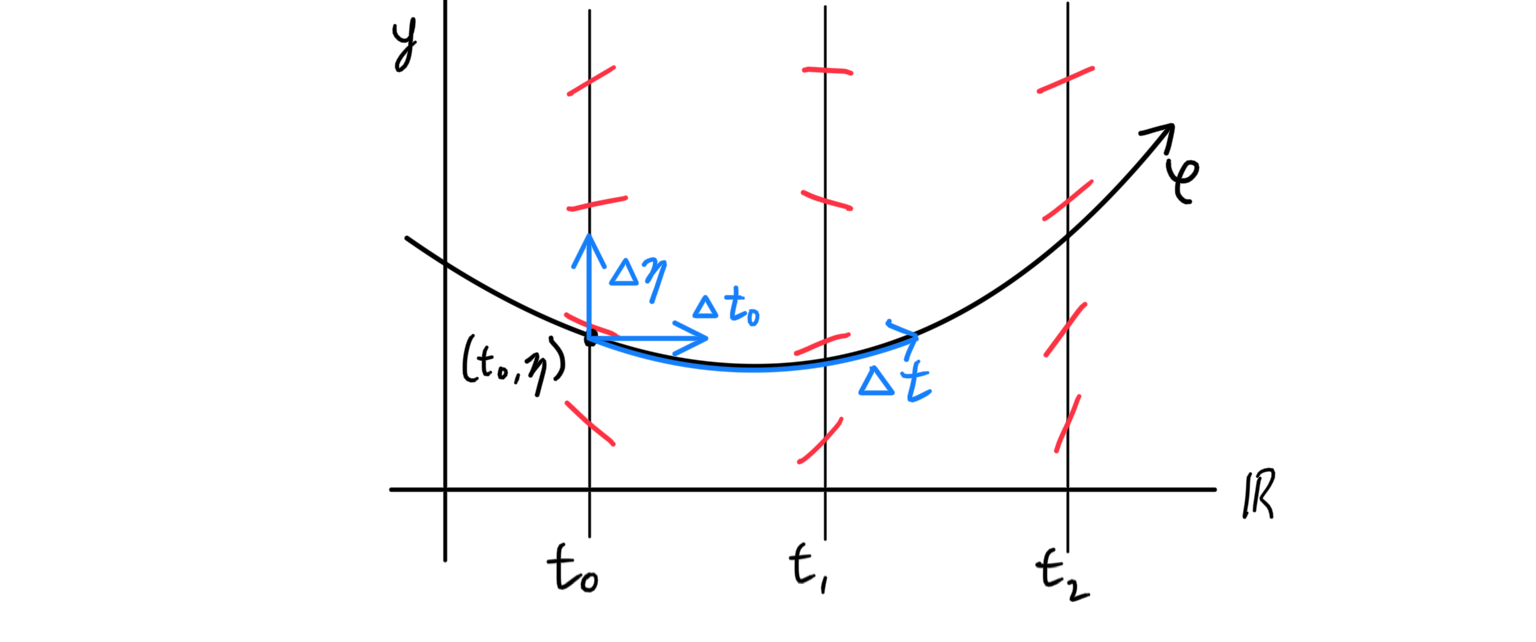
\includegraphics[scale=0.25]{img/Continuous_w_respect_to_3_things.PNG}
    \end{center}
    \end{theorem}

    We briefly state a useful result. 

    \begin{lemma}[Gronwall Inequality]
    Let $K \geq 0$ be a constant and $f, g$ be nonnegative $C^0$ functions on some interval $\alpha \leq t \leq \beta$ satisfying the inequality
    \[f(t) \leq K + \int_\alpha^t f(s) g(s) \, ds \text{ for } \alpha \leq t \leq \beta\]
    Then, 
    \[f(t) \leq K \exp \bigg( \int_{\alpha}^t g(s) \,ds \bigg) \text{ for } \alpha \leq t \leq \beta\]
    \end{lemma}

  \subsection{Linear Systems of DEQs}

    Remember that higher-order systems can be reduced to a system of first-order DEQs, so it makes sense to talk about a system of first-order linear DEQs. 

    \begin{definition}[Linear Systems of DEQs]
    The system $y^\prime = f(t, y)$ linear in the components of $y$ has the form 
    \begin{align*}
        y_1^\prime & = a_{11}(t) y_1 + a_{12}(t) y_2 + \ldots + a_{1n}(t) y_n + g_1 (t) \\
        y_2^\prime & = a_{21}(t) y_1 + a_{22}(t) y_2 + \ldots + a_{2n}(t) y_n + g_2 (t) \\
        \vdots & = \vdots \\
        y_n^\prime & = a_{n1}(t) y_1 + a_{n2}(t) y_2 + \ldots + a_{nn}(t) y_n + g_n (t)
    \end{align*}
    which can be represented as a matrix equation, where $A: \mathbb{R} \longrightarrow \text{Mat}(n \times n, \mathbb{R}), g: \mathbb{R} \longrightarrow \mathbb{R}^n$. 
    \[y^\prime = A(t) y + g(t) \iff \begin{pmatrix}
    y_1 \\ y_2 \\ \vdots \\ y_n
    \end{pmatrix}^\prime = \begin{pmatrix}
    a_{11}(t) & a_{12} (t) & \ldots & a_{1n}(t) \\
    a_{21}(t) & a_{22} (t) & \ldots & a_{2n}(t) \\
    \vdots & \vdots & \ddots & \vdots \\
    a_{n1}(t) & a_{n2} (t) & \ldots & a_{nn}(t) 
    \end{pmatrix} \begin{pmatrix}
    y_1 \\ y_2 \\ \vdots \\ y_n
    \end{pmatrix} + \begin{pmatrix}
    g_1 (t) \\ g_2 (t) \\ \vdots \\ g_n (t) 
    \end{pmatrix}\]
    \end{definition}

    It is actually true that there exists a unique solution to this linear system as long as $\eta$ is finite. This is formalized in the theorem below. 

    \begin{theorem}[Existence of Unique Solutions of Linear Systems]
    Let matrix-valued function $A(t)$ and vector valued function $g(t)$ be continuous on some interval $a \leq t \leq b$. Then, if $a\leq t_0 \leq b$ and if $|\eta| < \infty$, the system of linear DEQs
    \[y^\prime = A(t) y + g(t)\]
    has a unique solution $y = \varphi(t)$ satisfying initial condition $\varphi(t_0) = \eta$ and existing on the interval $a \leq t \leq b$. 
    \end{theorem}

    \subsubsection{Homogeneous Linear Systems of DEQs}

      Note that a first-order homogeneous linear system is of form 
      \[y^\prime = A(t) y\]
      Note that the scalar analogue of a homogeneous first-order linear DEQ can be changed to the above form as such 
      \begin{align*}
          a_0 (t) y^\prime + a_1 (t) y = 0 & \implies a_0 (t) y^\prime = - a_1 (t) y \\
          & \implies y^\prime = -\frac{a_1 (t)}{a_0 (t)} y
      \end{align*}
      where we treat $y, y^\prime$ as $1$-dimensional vectors, and $-a_1(t)/a_0 (t)$ as a $1 \times 1$ matrix. 

      Just as in the scalar case, the solutions to the linear system forms a vector space. 

      \begin{theorem}[Fundamental Set of Solutions]
      Given the first-order linear homogeneous system 
      \[y^\prime = A(t) y\]
      with $A: \mathbb{R} \longrightarrow \text{Mat}(n \times n, \mathbb{C})$ being continuous over interval $I \subset \mathbb{R}$, the solutions of this system over $I$ form an $n$-dimensional subspace within $C^1(\mathbb{R}, \mathbb{C}^n)$, the space of all continuously differentiable functions mapping $\mathbb{R} \longrightarrow \mathbb{C}^n$. The basis of this space is called the \textit{fundamental set of solutions}. 
      \end{theorem}
      \begin{proof}
      We can rearrange the system as 
      \begin{align*}
          -y_1^\prime + a_{11}(t) y_1 + a_{12}(t) y_2 + \ldots + a_{1n}(t) y_n = 0 \\
          -y_2^\prime + a_{21}(t) y_1 + a_{22}(t) y_2 + \ldots + a_{2n}(t) y_n = 0 \\
          \vdots = \vdots \\
          -y_n^\prime + a_{n1}(t) y_1 + a_{n2}(t) y_2 + \ldots + a_{nn}(t) y_n = 0 
      \end{align*}
      and put it into matrix form
      \[\begin{pmatrix}
      a_{11}(t) & \ldots & a_{1n} (t) & -1 & \ldots & 0 \\
      \vdots & \ddots &\vdots (t) & \vdots & \ddots& \vdots \\
      a_{n1}(t) & \ldots & a_{nn} (t) & 0 & \ldots & -1 
      \end{pmatrix} \begin{pmatrix}y_1  \\ \vdots \\ y_n \\ y_1^\prime \\ \vdots \\ y_n^\prime \end{pmatrix} = 0\]
      The kernel of this linear mapping has dimension $n$. 
      \end{proof}

      \begin{example}[4th Order DEQ into System of 1st-Order DEQs in Matrix Form]
      We can write the following homogeneous 4th order differential equation 
      \[y^{(4)} + 3 y^{\prime\prime} - \sin{(t)} y^\prime + 8y = t^2, \;\; y(0) = 1, y^\prime (0) = 2, y^{\prime\prime} (0) = 3, y^{(3)} (0) = 4 \]
      into the system by making the substitutions 
      \begin{align*}
          & x_1 = y \implies x_1^\prime = y^\prime = x_2 \\
          & x_2 = y^\prime \implies x_2^\prime = y^{\prime\prime} = x_3 \\
          & x_3 = y^{\prime\prime} \implies x_3^\prime = y^{(3)} = x_4 \\
          & x_4 = y^{(3)} \implies x_4^\prime = y^{(4)} = -8y + \sin{(t)} y^\prime - 3y^{\prime\prime} + t^2 = -8x_1 + \sin{(t)} x_2 - 3x_3 + t^2
      \end{align*}
      which leads to the matrix equation
      \[x^\prime =  \begin{pmatrix} 
      0&1&0&0\\
      0&0&1&0\\
      0&0&0&1\\
      -8&\sin(t)&-3&0
      \end{pmatrix} x
      + \begin{pmatrix} 
      0\\0\\0\\t^2
      \end{pmatrix}, x (0) = \begin{pmatrix} 
      1\\2\\3\\4
      \end{pmatrix}\]
      \end{example}

      \begin{definition}[Solution Matrix, Fundamental Matrix]
      Given that $\varphi_1, \varphi_2, \ldots, \varphi_n: \mathbb{R} \longrightarrow \mathbb{R}^n$ are $n$ solutions to the homogeneous matrix differential equation $y^\prime = A(t) y$, the $n \times n$ matrix whose columns are solutions is called a \textit{solution matrix}.

      Then $n \times n$ matrix with its columns being the $n$ linearly independent solutions on $I$ is called the \textit{fundamental matrix}. 
      \[\Phi = \begin{pmatrix}
      | & | & \ldots & | \\
      \phi_1 & \phi_2 & \ldots & \phi_n \\
      | & | & \ldots & |
      \end{pmatrix} = \begin{pmatrix}
      \phi_{11}(t) & \phi_{21} (t) & \ldots & \phi_{n1} (t) \\
      \phi_{12} (t) & \phi_{22} (t) & \ddots & \phi_{n2} (t) \\
      \vdots & \vdots & \ddots & \vdots \\
      \phi_{1n} (t) & \phi_{2n} (t) & \ldots & \phi_{nn} (t)
      \end{pmatrix}\]
      Note that a fundamental matrix is not unique (that is, two different fundamental matrices $\Phi, \Tilde{\Phi}$ can exist), but since the column space of $\Phi$ and $\Tilde{\Phi}$ are the same, we can change any fundamental matrix into another with a linear change of basis. That is, given the passive transformation matrix $P$, 
      \[\Phi = P^{-1} \Tilde{\Phi} P\]
      Furthermore, the fundamental matrix $\Phi (t)$ has the property that any solution of the matrix DEQ can be expressed as a linear combination of the column space of $\Phi(t)$. That is, every solution $\psi (t)$ can be constructed as
      \[\psi (t) = \Phi (t) c, \;\;\; c = \begin{pmatrix} 
      c_1 \\ \vdots \\ c_n \end{pmatrix} \]
      \end{definition}

      \begin{theorem}[Abel's Formula]
      If $\Phi$ is a solution matrix of $y^\prime = A(t) y$ on $I$ and if $t_0$ is any point of $I$, then 
      \[\det{\Phi(t)} = \det{\Phi(t_0)} \exp\bigg( \int_{t_0}^t \sum_{j=1}^n a_{jj} (s) \, ds\bigg) \text{ for every } t \in I\]
      It immediately follows that since $t_0$ is arbitrary, either 
      \begin{enumerate}
          \item $\det{\Phi(t)} \neq 0$ for each $t \in I$, or 
          \item $\det{\Phi(t)} = 0$ for every $t \in I$ 
      \end{enumerate}
      \end{theorem}

      \begin{corollary}
      A solution matrix $\Phi$ of the matrix equation 
      \[y^\prime = A(t) y\]
      on interval $I$ is a fundamental matrix if and only if 
      \[\det{\Phi(t)} \neq 0 \text{ for every } t \in I\]
      Practically, this means that to test whether a solution matrix is a fundamental matrix, it suffices to evaluate its determinant at one point! 
      \end{corollary}

      Note that this corollary has a very close relationship with the previously mentioned theorem on how the Wronskian is used to determine the linear independence of solutions to a linear DEQ $\mathcal{L}_n (y) = 0$. More specifically, if we take a $n$th order linear DEQ satisfying the hypothesis of the Wronskian theorem, we can change it to a system of first-order linear equations and apply the previous corollary to determine linear independence of solutions. Both approaches are exactly the same. 

    \subsubsection{Linear Inhomogeneous Systems}

      It is obvious that due to the \textit{forcing term} $g(t)$ (representing the external force on the system), the form of solution of the inhomogeneous system 
      \[y^\prime = A(t) y + g(t)\]
      is 
      \[\varphi(t) = \psi(t) + \Phi(t) c\]
      where $\psi$ is a special solution to the DEQ over interval $I$. Since we know how to find the fundamental matrix $\Phi$, all it remains is to find $\psi$. We can do this using the multivariate variation of constants formula. 

      For notational purposes, we write for vector valued functions $f: \mathbb{R} \longrightarrow \mathbb{R}^n$, where $f_1, f_2, \ldots, f_n$ are the basis functions, 
      \[\int_a^b f(x)\,ds = \begin{pmatrix}
      \int_a^b f_1 (x)\,ds \\ \vdots \\ \int_a^b f_n(x)\,ds
      \end{pmatrix}\]

      \begin{theorem}[Multivariate Variation of Constants Formula]
      Given the inhomogeneous first-order linear system 
      \[y^\prime = A(t) y + g(t)\]
      if $\Phi$ is the fundamental matrix of its homogeneous counterpart $y^\prime = A(t) y$ on interval $I \subset \mathbb{R}$, then the special function given by the variation of constants formula 
      \[\psi (t) = \Phi (t) \int_{t_0}^t \Phi^{-1} (s) g(s) \,ds\]
      is the unique solution of the original DEQ satisfying the initial condition on $I$
      \[\psi (t_0) = 0\]
      (Notice that $\Phi^{-1}$ is always well defined since $\Phi$ is nonsingular) This means that every solution $\phi$ of the DEQ has the form 
      \[\phi(t) = \psi (t) + \phi_h (t)\]
      where $\varphi_h$ is the solution of the homogeneous system satisfying the same initial condition at $t_0$ as $\varphi$ (e.g. $\varphi_h (t_0) = \eta$). This makes it such that the initial conditions are met: 
      \[\varphi(t_0) = \psi(t_0) + \varphi_h (t_0) = 0 + \eta = \eta\]
      \end{theorem}

  \subsection{Linear Systems with Constant Coefficients}

    If the homogeneous system 
    \[y^\prime = A(t) y\]
    has constant coefficients (i.e. $A$ consists of constant terms), then we can obtain an explicit formula of the fundamental matrix. 

    Also, to reduce confusion, 
    \begin{enumerate}
        \item $Ax$ will be used to denote matrix $A$ multiplied by vector $x$
        \item $xA$ will be used to denote scalar $x$ multiplied to matrix $A$ (row vector multiplication will not be seen in this section)
    \end{enumerate}

    \begin{theorem}[Fundamental Matrix of a Linear System with Constant Coefficients]
    Given the system of $n$ linear equations 
    \[y^\prime = A y, \;\;\;\;\; A \in \text{Mat}(n \times n, \mathbb{C})\]
    the matrix
    \[\Phi(t) = e^{(t-t_0)A} = \sum_{m=0}^\infty \frac{((t-t_0)A)^m}{m!}\]
    is the fundamental matrix with $\Phi(t_0) = I$ on $(-\infty, \infty)$. 
    \end{theorem}
    \begin{proof}
    $\Phi(t_0) = I$ is obvious from substitution. Assuming $t_0 = 0$, we differentiate $At: \mathbb{R} \longrightarrow \text{Mat}(n \times n, \mathbb{R})$ with respect to $t$ to get
    \[\big( e^{tA} \big)^\prime = A + \frac{tA^2} {1!} + \frac{t^2 A^3}{2!} + \ldots + \frac{t^{k-1} A^{k}}{(k-1)!} + \ldots = A e^{tA}\]
    This means that given any constant vector $c \in \mathbb{R}^n$, we have
    \[\big( e^{tA} \big)^\prime c = A e^{tA} c \implies \big( e^{tA} c\big)^\prime = A (e^{tA} c)\]
    and so $e^{tA}$ is a solution matrix. Furthermore, since $\det{ \Phi(0)} = \det{I} = 1$, it is a fundamental matrix (by the corollary to Abel's formula). 
    \end{proof}

    Note that given an arbitrary matrix $A$, it is stupid to calculate $e^{A}$ explicitly. Rather, we can use a change of basis to put it into Jordan Canonical Form $J$. 
    \[A = P^{-1} J P\]
    Then, it is clear that
    \[e^A = e^{P^{-1} J P} = P^{-1} e^J P\]
    Finding the eigendecomposition of a linear mapping, which may require working over the field $\mathbb{C}$ (or by introducing generalized eigenvectors over $\mathbb{R}$). This entire process is talked in detail in the linear algebra chapter. 

    Another trick that may work in some cases is the following lemma. 

    \begin{lemma}
    If two $n \times n$ matrices commute, then
    \[e^{M} \cdot e^{P} = e^{M + P} \]
    \end{lemma}
    \begin{proof}
    Trivial using the Baker-Campbell-Hausdorff formula. 
    \end{proof}

    Finally, we mentioned a greatly simplified variation of constants formula for the case when we solve a inhomogeneous system of linear DEQs with constant coefficients. 

    \begin{corollary}[Multivariate Variation of Constants Formula for Constant Coefficient Systems]
    Given inhomogeneous system of $N$ linear DEQs 
    \[y^\prime = A y + g(t), \;\;\;\;\; A \in \text{Mat}(n \times n, \mathbb{R}), g \in C^0\]
    with initial conditions $\varphi(t_0) = \eta$, then a specific solution of the system is 
    \[\psi (t) = \int_{t_0}^t e^{(t-s)A} g(s) \,ds , \text{ where } \psi(t_0) = 0\]
    meaning that the general solution to this equation is 
    \[\varphi(t) = e^{(t - t_0)A} \eta + \int_{t_0}^t e^{(t-s)A} g(s) \,ds \;\;\;\;\; -\infty < t< \infty\]
    where $\varphi(t_0) = \eta$. 
    \end{corollary}

    \begin{example}
    Given the initial value problem 
    \[y^\prime = Ay + g(t) \iff \begin{pmatrix} y_1 ^\prime \\ y_2^\prime \end{pmatrix} = \begin{pmatrix} 2 & 1 \\ -1 & 4 \end{pmatrix} \begin{pmatrix} y_1 \\ y_2 \end{pmatrix} + \begin{pmatrix} e^{3t} \\ 1 \end{pmatrix}, \;\;\; \varphi(0) = \eta\]
    Then, we have
    \begin{align*}
        \Phi(t) & = e^{tA} = e^{3t} \begin{pmatrix} 1-t & t \\ -t & 1+t \end{pmatrix} \\
        \Phi(t) \Phi^{-1} (s) & = e^{(t-s)A} = e^{3(t-s)} \begin{pmatrix} 1 - (t-s) & t-s \\ -(t-s) & 1+(t-s) \end{pmatrix} \\
        e^{(t-s)A} g(s) & = e^{3t} \begin{pmatrix}
        1-(t-s)+e^{-3s}(t-s) \\ -(t-s) + e^{-3s} (1+t-s)\end{pmatrix}
    \end{align*}
    Therefore, 
    \[\varphi(t) = e^{3t} \begin{pmatrix} 1-t & t \\ -t & 1+t \end{pmatrix} \eta + e^{3t} \int_{0}^t \begin{pmatrix} 1-(t-s) + e^{-3s} (t-s) \\
    -(t-s) + e^{-3s}(1+t-s) \end{pmatrix} \,ds\]
    which can be easily evaluated. 
    \end{example}

    \subsubsection{Asymptotic Behavior of Solutions}

      In many cases, in order to apply the variation of constants formula 
      \[\varphi(t) = e^{(t - t_0)A} \eta + \int_{t_0}^t e^{(t-s)A} g(s) \,ds \;\;\;\;\; -\infty < t< \infty\]
      and others derived from it, we must know how the matrix $e^{tA}$ behaves. For example, in order to measure the growth of solutions of as $t \rightarrow \infty$, we need to estimate 
      \[\lim_{t\rightarrow \infty} \varphi(t)\]
      where $|\cdot|$ is the L-1 norm. But this cannot be done without knowing a useful estimate of $|e^{tA}|$. 

      \begin{theorem}
      Given $\lambda_1, \lambda_2, \ldots, \lambda_k$ are distinct eigenvalues of $A$, where $\lambda_j$ has multiplicity $n_j$ and $n_1 + \ldots + n_k = n$, let $\rho$ be any real number such that 
      \[\rho > \max_{j=1, \ldots, k} \big( \text{Re}(\lambda_i)\big)\]
      Then, there exists a constant $K > 0$ such that
      \[|e^{tA}| \leq K e^{t \rho} \text{ for } 0 \leq t < \infty\]
      \end{theorem}

      Its applications really lies within its corollary. 

      \begin{corollary}
      If all eigenvalues of $A$ have real parts negative, then every solution $\varphi(t)$ of the system
      \[y^\prime = A y\]
      approaches $0$ as $t \rightarrow + \infty$. More precisely, there exists constants $\Tilde{K} > 0$, $\sigma > 0$ such that
      \[|\varphi(t)|< \Tilde{K} e^{-\sigma t}, \;\;\; (0 \leq t < \infty)\]
      \end{corollary}

      \begin{theorem}[Upper Bound on Growth Rate of Solutions of Nonhomogeneous Linear System with Constant Coefficients]
      Suppose that in the linear inhomogeneous system 
      \[y^\prime = A y + g(t)\]
      the function $g(t)$ grows no faster than an exponential function; that is, there exists real constants $M > 0, T \geq 0$, and $a \in \mathbb{R}$ such that
      \[|g(t)| \leq M e^{at} \text{ for all } t \geq T\]
      Then, every solution $\varphi$ of the system grows no faster than an exponential function. That is, there exists real constants $K>0, b$ such that
      \[|\varphi(t)| \leq K e^{bt} \text{ for all } t \geq T\]
      The derivative $\varphi^\prime (t)$ also grows no faster than an exponential function. 
      \end{theorem}

\section{Laplace Transforms}

  Laplace transforms extends our toolkit for solving linear differential equations (and systems of them) by reducing an initial value problem into an algebra problem, which can be summarized by the diagram below, where $\mathcal{L}$ represents the transform. 
  \[
    \begin{tikzcd}
      \text{Algebra Problem} \arrow{r}{solution} &  Y(t)\\
      \text{DEQ Problem} \arrow{u}{\mathcal{L}} \arrow{r}{solution} & y = \varphi(t) \arrow{u}{\mathcal{L}}
    \end{tikzcd}
  \]
  Laplace transforms also allows us to work with piecewise continuous functions. 

  The method of Laplace Transforms does not actually allow us to solve new types of differential equations. Rather, it is useful because it enables us to find one particular solution of the differential equation which satisfies the initial conditions directly, rather than first finding the general solution and then using the initial conditions to determine constants. 

  \begin{definition}[Functions of exponential growth at infinity]
  A function on $0 < t < \infty$ is said to be \textit{of exponential growth at infinity} if it satisfies
  \[|f(t)| \leq M e^{ct}\]
  for some real constants $M>0$ and $c$, for all sufficiently large $t$. 
  \end{definition}

  \begin{definition}[Function Class $\Lambda$]
  The \textit{class $\Lambda$} of functions is defined as those functions on $0<t<\infty$ which are
  \begin{enumerate}
      \item absolutely integrable on $0$ 
      \item piecewise continuous on $(0, \infty)$
      \item of exponential growth at infinity
  \end{enumerate}
  Clearly, the functions $1, t, t^n (n \in \mathbb{N}), \sin{t}, \cos{t}, e^{zt} (z \in \mathbb{C})$ are in class $\Lambda$, but $e^{t^2} \not\in \Lambda$. 
  \end{definition}

  \begin{definition}[Laplace Transform]
  Let $f \in \Lambda$. The \textit{Laplace transform} of $f$ is denoted $\mathcal{L}\{f(t)\}$ or $F(t)$, defined
  \[F(s) \equiv \int_0^\infty f(t)e^{-s t} \, dt = \lim_{A \rightarrow \infty} f(t) e^{-st}\,dt \]
  Sometimes, the Laplace transform may be defined by setting the lower limit to $- \infty$. 
  \[F(t) \equiv \int_{-\infty}^\infty f(t) e^{-s t}\,dt\]
  \end{definition}

  \begin{example}
  The Laplace transformation of constant function $1$ is 
  \[\int_0^\infty e^{-st}\,dt = \lim_{A \rightarrow \infty} \int_0^A e^{-st} \,dt = \lim_{A \rightarrow \infty} \bigg( \frac{1}{s} - \frac{e^{-sA}}{s} \bigg) = \frac{1}{s}\;\;\;\; (\text{Re}(s) > 0)\]
  Clearly, the integral does not converge for Re$(s) \leq 0$. The Laplace transform of $e^{zt}$ is
  \[\mathcal{L} (e^{zt}) = \frac{1}{s-z} \;\;\;\; (\text{Re}(s)> \text{Re}(z))\]
  \end{example}

  From the examples before and our notation of the transform, we can see and prove the following. 

  \begin{proposition}[Linearity of the Laplace Transform]
  The Laplace transform is a linear map with respect to its function argument. That is, 
  \[\mathcal{L} \{a f + b g\} = a \mathcal{L}\{f\} + b \mathcal{L}\{g\}\]
  This means that if $f: \mathbb{R} \longrightarrow \mathbb{C}$ is a complex-valued function
  \[f(t) = u(t) + i v(t)\]
  Then, 
  \[\mathcal{L}\big(f(t)\big) = \mathcal{L}\big(u(t) + i v(t) \big) = \mathcal{L} \big( u(t) \big) + i \mathcal{L} \big( v(t)\big)\]
  That is, 
  \[\text{Re}\big((\mathcal{L}(f(t))\big) = \mathcal{L}( \text{Re}(f(t))), \text{Com}\big((\mathcal{L}(f(t))\big) = \mathcal{L}( \text{Com}(f(t)))\]
  \end{proposition}


  \subsection{Common Laplace Transforms}

    \begin{example}
    Given $z = \alpha + i \beta \in \mathbb{C}$, with $\alpha, \beta \in \mathbb{R}$, and $f(t) = e^{zt}$, we have
    \begin{align*}
        \mathcal{L} (e^{zt}) & = \mathcal{L} (e^{\alpha t} e^{i \beta t}) = \mathcal{L} \big( e^{\alpha t} \cos{\beta t} + i e^{\alpha t} \sin{\beta t}\big) \\
        & = \frac{1}{s-z} = \frac{1}{z - \alpha - i \beta} \\
        & = \frac{s - \alpha + i \beta}{(s-\alpha)^2 + \beta^2}
    \end{align*}
    By linearity, we can take the real and complex parts of this transform to get
    \begin{align}
        \mathcal{L} \big(e^{\alpha t} \cos{\beta t} \big) & = \frac{s-\alpha}{(s-\alpha)^2 + \beta^2} \\
        \mathcal{L} \big(e^{\alpha t} \sin{\beta t} \big) & = \frac{\beta}{(s-\alpha)^2 + \beta^2}
    \end{align}
    Taking $\alpha = 0$ gives us
    \[\mathcal{L} \big( \cos{\beta t}\big) = \frac{s}{s^2 + \beta^2}, \;\;\; \mathcal{L}\big( \sin{\beta t}\big) = \frac{\beta}{s^2 + \beta^2} \;\;\; \text{Re}(s) > 0\]
    \end{example}

    To compute the Laplace transforms functions of some other forms, we can use the following theorem. 

    \begin{theorem}
    The Laplace transform of a function $f$ in the class $\Lambda$ has derivatives of all orders, given by
    \[F^{(k)} (s) = (-1)^k \int_0^\infty t^k e^{-st} f(t)\,dt, \;\;\;\; k = 1, 2, \ldots\]
    Furthermore, $f(t) \in \Lambda \implies t^k f(t) \in \Lambda$ for every positive integer $k$, and its Laplace transform is given by
    \[\mathcal{L}\big( t^k f(t) \big) = (-1)\]
    \end{theorem}

    \begin{corollary}
    It follows immediately that
    \begin{align*}
        \mathcal{L}\big( t^k\big) & = (-1)^k \frac{d^k}{d s^k} \bigg( \frac{1}{s} \bigg) = \frac{k!}{s^{k+1}} \;\;\; (\text{Re}(s) > 0) \\
        \mathcal{L}\big( t^k e^{zt}\big) & = (-1)^k \frac{d^k}{ds^k} \bigg( \frac{1}{s-z} \bigg) = \frac{k!}{(s-z)^{k+1}} \;\;\; (\text{Re}(s) > \text{Re}(z))
    \end{align*}
    \end{corollary}

    Another theorem for computing Laplace transforms. 

    \begin{theorem}
    If the function $f \in \Lambda$ has a Laplace transform $F$, then for any constant $a \in \mathbb{C}$, 
    \[\mathcal{L}\big(e^{at} f(t) \big) = F(s-a)\]
    \end{theorem}
    \begin{proof}
    It is easy to prove that $e^{at} f(t) \in \Lambda$, since 
    \[|f(t)| \leq M e^{ct} \implies |e^{at} f(t)| \leq e^{\alpha t} M e^{ct} = M e^{(a+c)t}\]
    and thus $e^{at} f(t)$ is of exponential growth at infinity. Calculating the Laplace transform, we get
    \[\mathcal{L}\big(e^{at} f(t) \big) = \int_0^\infty e^{-st} e^{at} f(t) \,dt = \int_0^\infty e^{-(s-a)t} f(t) \,dt = F(s - a)\]
    \end{proof}

    We conclude this subsection by providing a table of common Laplace transforms. 

    \begin{theorem}[Table of Common Laplace Transforms]
    Here we have some common transforms, where $a \in \mathbb{R}$ is a constant. Note that the gamma function
    \[\Gamma(t) \equiv \int_{0}^\infty e^{-x} \, x^{t-1}\,dx\]
    is an extension of the factorial function to the real numbers. 
    \begin{enumerate}
        \item $f(t) = e^{a t} \implies F(t) = \frac{1}{s-a}$
        \item $f(t) = t^n, n \in \mathbb{N} \implies F(t) = \frac{n!}{s^{n+1}}$
        \item $f(t) = t^p, p > -1 \implies F(t) = \frac{\Gamma(p+1)}{t^{p+1}}$
        \item $f(t) = \sin(at) \implies F(t) = \frac{a}{t^2 + a^2}$
        \item $f(t) = \cos(at) \implies F(t) = \frac{t}{t^2 + a^2}$ 
        \item $f(t) = t \sin(at) \implies F(t) = \frac{2 a t}{(t^2 + a^2)^2}$
        \item $f(t) = t \cos(at) \implies F(t) = \frac{t^2 - a^2}{(s^2 + a^2)^2}$
        \item $f(t) = \sin(a t + b) \implies F(t) = \frac{t \sin(b) + a \cos(b)}{t^2 + a^2}$
        \item $f(t) = \cos(a t + b) \implies F(t) = \frac{t \cos(b) - a \sin(b)}{t^2 + a^2}$
    \end{enumerate}
    \end{theorem}

    \subsubsection{Laplace Transforms of Derivatives}

      Now that we know how to calculate Laplace transforms, we must extend this to derivatives of functions in order to integrate it within differential equations. 

      \begin{lemma}
      Let $f$ be a differentiable function in the class $\Lambda$ whose derivative also belongs to the class $\Lambda$, and let the Laplace transform of $f$ be $F$. Then, 
      \[\mathcal{L} \big( f^\prime (t) \big) = s F(s) - f(0) \]
      \end{lemma}
      \begin{proof}
      We use the definition of Laplace transform and integrate by parts to get 
      \begin{align*}
          \mathcal{L}\big( f^\prime (t) \big) & = \int_0^\infty e^{-st} f^\prime (t) \,dt = \lim_{A \rightarrow \infty} e^{-st} f^\prime (t) \,dt \\
          & = \lim_{A\rightarrow \infty} \bigg( e^{-st} f(t) \big|_0^A + \int_0^A s e^{-st} f(t)\,dt\bigg) \\
          & = - f(0) + s\int_0^\infty e^{-st} f(t) \,dt = s F(s) - f(0)
      \end{align*}
      where we used the fact ($f \in \Lambda \implies f$ is of exponential growth at infinity) that 
      \[\lim_{A \rightarrow \infty} e^{-sA} f(A) = 0\]
      for sufficiently large Re$(s)$. 
      \end{proof}

      \begin{definition}[The Class $\Lambda^k$]
      For each positive integer $k$, define $\Lambda^k$ to be the class of $C^k((0, \infty))$ (defined over $(0, \infty)$) functions in $\Lambda$ whose derivatives up to order $k$ also belong to $\Lambda$. That is, 
      \[\Lambda^k = \{f \in C^k((0, \infty))\;|\; f, f^\prime, f^{\prime\prime}, \ldots, f^{(k)} \in \Lambda \}\]
      \end{definition}

      \begin{theorem}[Laplace Transform of Derivatives]
      If $f \in \Lambda^k$ for some positive integer $k$, and if $F$ is the Laplace transform of $f$, then for any $1 \leq j \leq k$, 
      \begin{align*}
          \mathcal{L}\big( f^{(j)} (t) \big) & = s^j F(s) - \sum_{i=1}^j s^{j-i} f^{(i-1)}(0) \\
          & = s^j F(s) - s^{j-1} f(0) - s^{j-2} f^\prime (0) - \ldots - s f^{(j-2)}(0) - f^{(j-1)} (0)
      \end{align*}
      \end{theorem}
      \begin{proof}
      Using the lemma, proof by induction on $j$ for any fixed $k$. 
      \end{proof}

      Note that in order to solve a differential equation using Laplace transforms, we must know the initial values $\varphi(0), \varphi^\prime (0), \ldots$ at $t = 0$ (must be at $0$!) for us to simplify the algebraic equation that is produced. This is shown in the examples. 

      \begin{example}
      Given the first-order differential equation with initial conditions
      \[y^\prime + a y = 0, \;\;\; \varphi_0 (0) = y_0\]
      where $a, y_0$ are given constants. Assuming that the solution is in the class $\Lambda^1$, we try to find this using Laplace transforms. Let $Y_0 (s) = \mathcal{L}( \varphi_0)$. Then,
      \begin{align*}
          \mathcal{L}\big(\varphi_0^\prime (t) + a \varphi_0 (t)\big) & = \mathcal{L}\big(\varphi_0^\prime (t)\big) + a \mathcal{L}\big(\varphi_0 (t)\big) \\
          & = s Y_0 (s) - \varphi_0 (0) + a Y_0 (s) = 0
      \end{align*}
      So, 
      \[(s+a) Y_0 (s) = y_0 \implies Y_0 (s) = \frac{y_0}{s+a}\]
      Now the only problem remaining is to find a function whose Laplace transform is this expression. By direct verification, we can see that $\varphi_0 (t) = y_0 e^{-at}$ is indeed the solution. 
      \end{example}

      \begin{example}
      The Laplace transform of the nonhomogeneous first-order linear DEQ 
      \[y^\prime + a y= f(t), \;\;\; \varphi(0) = y_0\]
      is (where $Y(s) = \mathcal{L}(\varphi)$)
      \[s Y(s) - \varphi(0) + a Y(s) = F(s) \implies Y(s) = \frac{y_0}{s+a} + \frac{F(s)}{s+a}\]
      Therefore, we must find a function which has this expression as its Laplace transform. By the previous example, we know that $t_0 e^{-at}$ satisfies the first term, but we have no method as yet of finding a function whose Laplace transform is 
      \[\frac{F(s)}{s+a}\]
      This suggests that we will need a method of finding a function whose Laplace transform is the product of two given functions $F(s)$ and $1/(s+a)$. 
      \end{example}

      This final example shows what would happen if we tried to take the Laplace transform of linear DEQ with nonconstant coefficients. 

      \begin{example}
      Taking the Laplace transform of 
      \[y^\prime + 2t y = 0, \;\;\; \psi(0) = y_0\]
      gives (where $\mathcal{L}(\psi) = Z(s)$) 
      \[sZ(s) - \psi(0) - 2Z^\prime (s) = 0\]
      While in the previous problems the equation was greatly simplified into an algebraic problem, here we have a differential equation which is no simplier than the original problem. 
      \end{example}

      Clearly, this example suggests that the usefulness of the Laplace transform method is limited mainly to equations with constant coefficients. 

  \subsection{Heaviside Step, Dirac Delta Functions}

    \begin{definition}[Heaviside Step Function]
    A \textit{Heaviside (step) function}, denoted as $H$, $\mathbb{I}$, or $u$, is defined
    \[H(x) \equiv \begin{cases}
    0 & x < 0 \\
    1  & x \geq 0
    \end{cases}\]
    Clearly, it can be horizontally translated $c$ units to result in the function $H(t-c) = u_c$ which is $1$ if $t \geq c$ and $0$ otherwise. 
    \begin{center}
        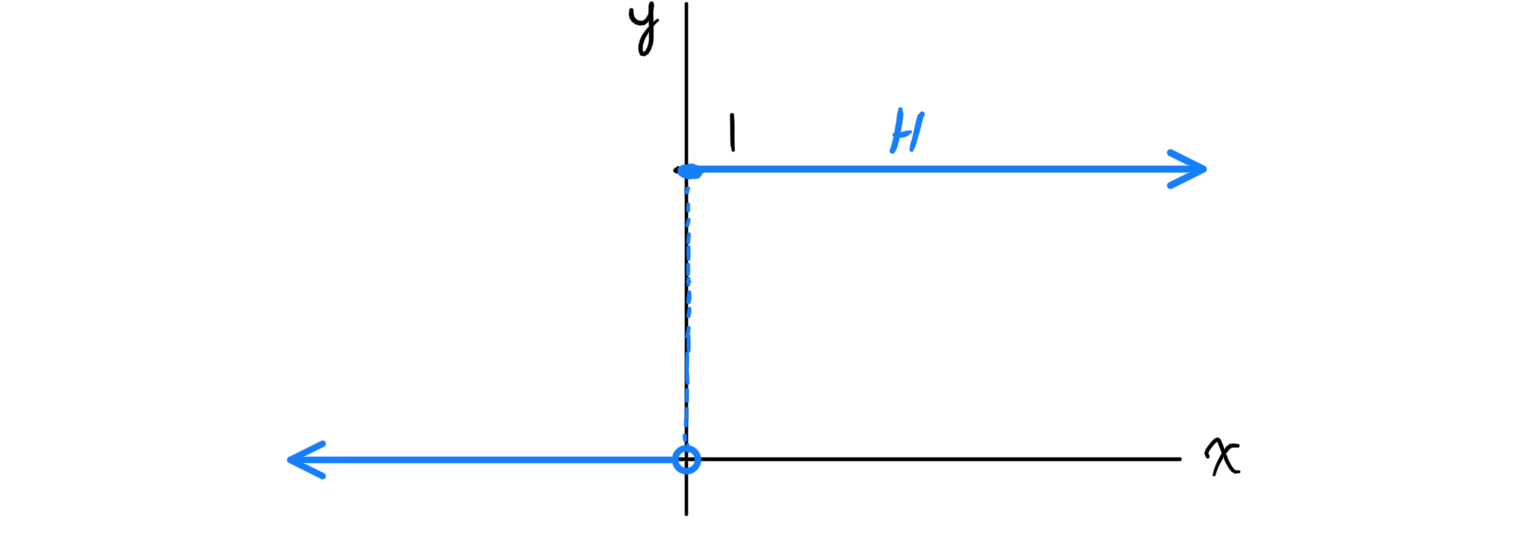
\includegraphics[scale=0.23]{img/Heaviside.PNG}
    \end{center}
    \end{definition} 

    Looking back a Heaviside step functions, we can combine them to create more complicated models. For example, we can redefine the piecewise function
    \[f(t) = \begin{cases}
    -4 & t < 6 \\
    25 & 6 \leq t < 8 \\
    16 & 8 \leq t < 30 \\
    10- & t \geq 30
    \end{cases}\]
    in terms of Heaviside functions as such
    \[f(t) = -4 + 29 u_6 (t) - 9 u_8 (t) - 6 u_{30} (t)\]
    This is analogous to a "switch" that we can turn on or off. Furthermore, we can use Heaviside functions to "shift" functions horizontally a certain length $c$ while turning them "off" for values of $t < c$ and "on" for values $t \geq c$. This can be written as 
    \[g(t) \equiv u_c (t) \, f(t - c)\]
    To find the Laplace transform of $g(t)$, we can evaluate it as such. 
    \begin{align*}
        \mathcal{L} \{u_c (t) \, f(t -c)\} & = \int_0^\infty e^{-s t} u_c (t) f(t-c) \,dt \\
        & = \int_c^\infty e^{-st} f(t-c) \,dt 
    \end{align*}
    Substituting $u = t - c$ gives
    \begin{align*}
         \mathcal{L} \{u_c (t) \, f(t -c)\} & = \int_0^\infty e^{-s (u+c)} f(u) \,du \\
         & = e^{-cs} \int_0^\infty e^{-su} f(u)\,du \\
         & = e^{-cs} F(s)
    \end{align*}
    This leads to the following formulas. 
    \begin{theorem}
    The Laplace transforms for Heaviside functions are:
    \begin{align*}
        & \mathcal{L} \{u_c (t) f(t-c)\} = e^{-ct} F(t) \\
        & \mathcal{L} \{u_c (t)\} = \frac{e^{-ct}}{t}
    \end{align*}
    \end{theorem}

    \begin{definition}[Dirac Delta Function]
    The \textit{Dirac delta function} is a generalized function or distribution that models forces exerted over small time frames. It can be thought of as a function $\delta$ satisfying the properties 
    \begin{align*}
        & 1. \delta (t - a) = 0, \;\; t \neq a \\
        & 2. \int_{a-\varepsilon}^{a+\varepsilon} \delta(t-a) \,dt, \;\; \varepsilon > 0 \\
        & 3. \int_{a-\varepsilon}^{a+\varepsilon} f(t) \delta(t-a) \,dt = f(a), \;\; \varepsilon > 0
    \end{align*}
    Alternatively, it may be evaluated as the limit of a Gaussian distribution centered at $a$ where $\sigma \rightarrow 0$. That is, 
    \[\delta(t) = \lim_{\sigma \rightarrow 0} \text{Normal}(a, \sigma^2)\]
    \begin{center}
        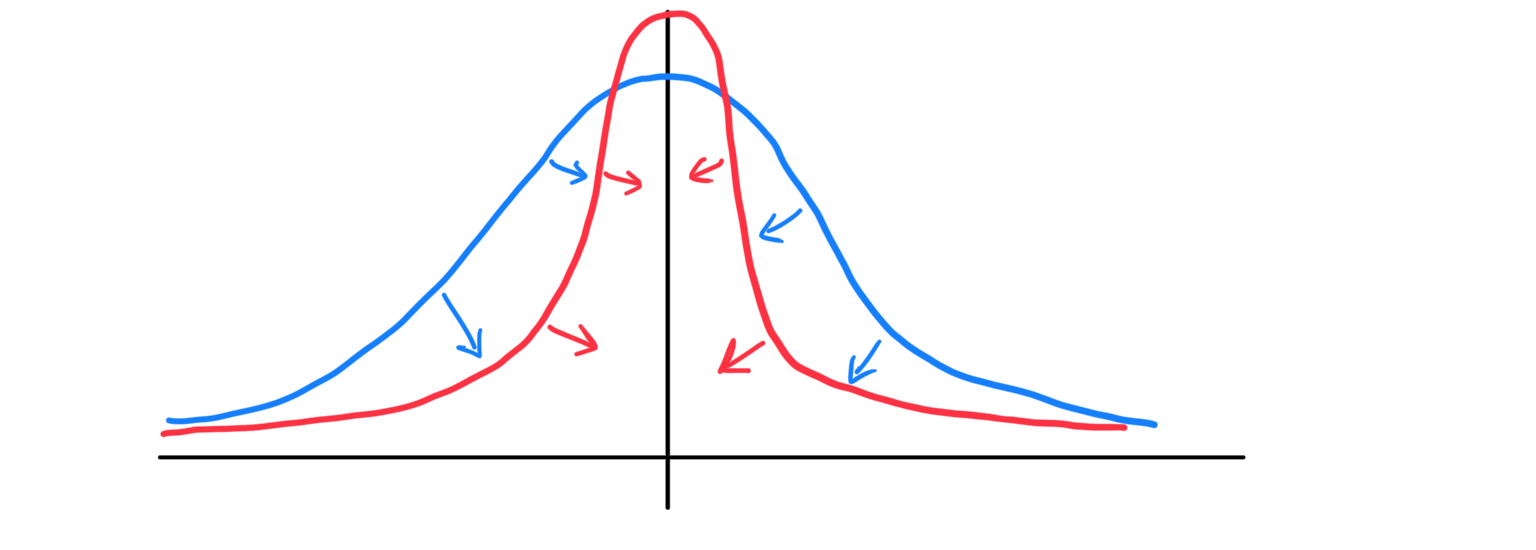
\includegraphics[scale=0.23]{img/Dirac_Delta.PNG}
    \end{center}
    \end{definition}

    To apply the Dirac delta function in Laplace transforms, we calculate
    \[\mathcal{L} \{ \delta(t-a)\} = \int_0^\infty e^{-st} \delta(t-a) \,dt = e^{-as}\]
    given that $a>0$. 

    \begin{proposition}
    More generally, we have
    \[\mathcal{L}\{u_c (t) f(t-c)\} = e^{-cs} F(s)\]
    where $F$ is the Laplace transform of $f$. 
    \end{proposition}

    \begin{lemma}
    The derivative of the Heaviside function $u_a (t)$ is the Dirac delta function centered at $a$. That is, 
    \[u_a^\prime (t) = \delta (t - a)\]
    \end{lemma}
    \begin{proof}
    With a bit of background in probability, the cumulative distribution function (CDF) of the Dirac delta function is defined
    \[\int_{-\infty}^t \delta(u - a)\,du = \begin{cases}
    0 & t < a \\
    1 & t \geq a
    \end{cases}\]
    But this is precisely the definition of the Heaviside function. By the fundamental theorem of calculus, we have
    \[u^\prime_a (t) = \frac{d}{d t} \int_{-\infty}^t \delta(u-a)\, du = \delta(t-a)\]
    \end{proof}

  \subsection{Inverse Laplace Transform}

    \begin{definition}[Inverse Laplace Transform]
    The \textit{Inverse Laplace transform} is the inverse of a Laplace transform. That is, 
    \[\mathcal{L}\big( f(t)\big) = F(s) \implies  \mathcal{L}^{-1} \big(F(s)\big) = f(t)\]
    \end{definition}

    Now, as we have mentioned in the previous examples, we would like to derive a certain method to find the inverse transform of a function. 

    \begin{theorem}[Inverse Laplace Transforms of Products of Functions]
    We assume that we are given two functions $f(t), g(t)$, with their Laplace transforms $\mathcal{f} = F(s), \mathcal{g} = G(s)$. Then, 
    \[\mathcal{L}\bigg(\int_0^t f(t-v) g(v)\,dv \bigg) = F(s)G(s)\]
    That is, given the function $F(s) G(s)$ (with their respective inverse transforms known), its inverse Laplace transform is
    \[\mathcal{L}^{-1} \big( F(s) G(s)\big) = \int_0^t f(t-v) g(v)\,dv\]
    given by the convolution integral of $f$ and $g$. 
    \end{theorem}
    \begin{proof}
    We let $H(s) = F(s) G(s)$ and try to find the function $h(t)$ where $\mathcal{L}(h) = H(s)$. If there is such as function $h$, then 
    \begin{align*}
        \mathcal{L}\big(h(t)\big) & = \int_0^\infty e^{-st} h(t)\,dt \\
        & = F(s) G(s) = \int_0^\infty e^{-su} f(u) \,du \int_0^\infty e^{-sv} g(v)\,dv
    \end{align*}
    where Re$(s)>\sigma = \max{(\alpha, \beta)}$, where $F(s) = \mathcal{L}(f)$ for Re$(s)>\alpha$ and $G(s) = \mathcal{L}(g)$ for Re$(s)>\beta$ ($\alpha, \beta \in \mathbb{R}$). Since each integral converges absolutely for Re$(s) > \sigma$, we can write the product of the two integrals as the iterated integral (using Fubini's theorem) 
    \begin{align*}
        \int_0^\infty e^{-st} h(t) \,dt & = \int_0^\infty \int_0^\infty e^{-s(u+v)} f(u) g(v)\,du \,dv \\
        & = \int_0^\infty g(v) \bigg(\int_0^\infty e^{-s(u+v)} f(u)\,du\bigg)\,dv \\
        & = \int_0^\infty g(v) \bigg( \int_0^\infty e^{-st} f(t-v) \,dt \bigg)\,dv \\
        & = \int_0^\infty e^{-st} \bigg( \int_0^t f(t-v) g(v)\,dv \bigg) \,dt
    \end{align*}
    where the second to last step was done by making the change of variable $u+v = t$ for Re$(s) > \sigma$. Therefore, 
    \begin{align*}
        F(s) G(s) & = \int_0^\infty e^{-st} h(t) \,dt = \int_0^\infty e^{-st} \bigg( \int_0^t f(t-v) g(v)\,dv \bigg) \,dt \\
        \implies & h(t) = \int_0^t f(t-v) g(v)\,dv
    \end{align*}
    \end{proof}

    \begin{proposition}
    $\mathcal{L}$ is a linear operator. 
    \[\mathcal{L}^{-1} \{ a F + b G\} = a \mathcal{L}^{-1} \{F\} + b \mathcal{L}^{-1} \{G\}\]
    \end{proposition}

    \begin{corollary}
    The only function in the class $\Lambda$ whose Laplace transform is identically $0$ is the zero function. 
    \end{corollary}

    \begin{example}
    We compute 
    \[\mathcal{L}^{-1} \bigg( \frac{1}{s^2 -1}\bigg) =\mathcal{L}^{-1} \bigg( \frac{1}{(s+1)(s-1)}\bigg)\]
    Since 
    \[\mathcal{L}^{-1} \bigg(\frac{1}{s-1}\bigg) = e^t, \; \mathcal{L}^{-1}\bigg(\frac{1}{s+1}\bigg) = e^{-t}\]
    we have
    \[\mathcal{L}^{-1} \bigg(\frac{1}{(s+1)(s-1)}\bigg) = \int_0^t e^{t-u} e^{-u} \,du = e^t \int_0^t e^{-2u} \,du = \frac{1}{2} \big(e^t - e^{-t}\big)\]
    We can also compute it using partial fraction decomposition and by using the linearity of $\mathcal{L}^{-1}$. 
    \begin{align*}
        \mathcal{L}^{-1} \bigg( \frac{1}{s^2-1}\bigg) & = \frac{1}{2} \Bigg( \mathcal{L}^{-1} \bigg( \frac{1}{s-1} \bigg) - \mathcal{L}^{-1} \bigg(\frac{1}{s+1}\bigg) \Bigg) \\
        & = \frac{1}{2} \big( e^t - e^{-t} \big) 
    \end{align*}
    \end{example}

    \begin{example}
    We compute 
    \[\mathcal{L}^{-1} \bigg( \frac{1}{s^2(s^2 + 1)}\bigg)\]
    we know that
    \[\mathcal{L}^{-1} \bigg(\frac{1}{s^2}\bigg) = t, \;\; \mathcal{L}^{-1} \bigg( \frac{1}{s^2+1}\bigg) = \sin{t}\]
    So,
    \[\mathcal{L}^{-1} \bigg( \frac{1}{s^2 (s^2+1)}\bigg) = \int_0^t (t-u) \sin{u} \,du = t \int_0^t \sin{u}\,du - \int_0^t u \sin{u}\,du = t - \sin{t}\]
    Using partial fractions, we have
    \[\mathcal{L}^{-1} \bigg(\frac{1}{s^2(s^2 + 1)} \bigg) = \mathcal{L}^{-1} \bigg( \frac{1}{s^2} \bigg) - \mathcal{L}^{-1} \bigg(\frac{1}{s^2 + 1} \bigg) = t - \sin{t}\]
    \end{example}

    \begin{example}
    Here is an example where we use only partial fractions. Since
    \[G(s) = \frac{86 s - 78}{(s+3) (s - 4) (5s - 1)} = -\frac{3}{s+3} + \frac{2}{s-4} + \frac{5}{5s-1}\]
    we have 
    \begin{align*}
        \mathcal{L}^{-1} \{G(s)\} & = \mathcal{L}^{-1} \{-\frac{3}{s+3} + \frac{2}{s-4} + \frac{5}{5s-1}\} \\
        & = -3 e^{-3t} + 2 e^{4 t} + e^{t/5}
    \end{align*}
    \end{example}

    Therefore, for rational functions of the form 
    \[\frac{N(s)}{D(s)}\]
    where $N, D$ are polynomials with the degree of $N$ less than the degree of $D$, we can take advantage of partial fractions to compute its inverse Laplace transform. 

    \begin{example}
    Solve the following differential equation. 
    \[2 y^{\prime\prime} + 3 y^\prime - 2y = t e^{-2t}, \;\; y(0) = 0, y^\prime (0) = -2\]
    We take the Laplace transforms of all the terms in the differential equation to get
    \[2\big( t^2 Y(t) - t y(0) - y^\prime (0)\big) + 3 \big( t Y(t) - y(0)\big) - 2 Y(t) = \frac{1}{(t+2)^2}\]
    which, after simplification, gives
    \[(2t^2 + 3t - 2) Y(t) + 4 = \frac{1}{(t+2)^2}\]
    Solving for $Y$, we get
    \begin{align*}
        Y(t) & = \frac{1}{(2t-1)(t+2)^3} - \frac{4}{(2t-1)(t+2)} \\
        & = \frac{1}{125} \bigg(\frac{-96}{s-\frac{1}{2}} + \frac{96}{s+2} - \frac{10}{(s+2)^2} - \frac{25}{(s+2)^3} \bigg)
    \end{align*}
    The inverse transform of this gives 
    \[y(t) = \frac{1}{125} \Big( -96 e^{\frac{t}{2}} + 96 e^{-2t} - 10t e^{-2t} - \frac{25}{2} t^2 e^{-2t}\Big) \]
    \end{example}

    We now deal with Heaviside functions in this next example. 
    \begin{example}
    Solve the following initial value problem. 
    \[2 y^{\prime\prime} + 10 y = 3 u_{12} (t) - 5 \delta(t - 4), \;\; y(0) = -1, y^\prime (0) = -2\]
    We take the Laplace transform 
    \begin{align*}
        & 2 \big( t^2 Y(t) - t y(0) - y^\prime (0) \big) + 10 Y(t) = \frac{3 e^{-12t}}{t} - 5 e^{-4 t} \\
        \implies & (2 t^2 + 10) Y(t) + 2t + 4 = \frac{3 e^{-12t}}{t} - 5 e^{-4t}
    \end{align*}
    and solve for $Y$
    \begin{align*}
        Y(t) & = 3 e^{-12t} \bigg(\frac{1}{t (2t^2 + 10)} \bigg) - 5e^{-4t} \bigg(\frac{1}{2t^2 + 10} \bigg) - \frac{2t+4}{2t^2 + 10} \\
        & = 3 e^{-12t} \bigg(\frac{1}{10t} - \frac{1}{10(t^2+5)} \bigg) - 5e^{-4t} \bigg(\frac{1}{2t^2 + 10} \bigg) - \frac{2t+4}{2t^2 + 10} \\
        & = 3 e^{-12t} F(t) - 5 e^{-4t} G(t) - H(t)
    \end{align*}
    Using the rules for inverse transforming Dirac delta functions, we can get
    \[y (t) = 3 u_{12} (t) f(t-12) - 5 u_4 (t) g(t-4) - h(t)\]
    where 
    \begin{align*}
        & f(t) = \frac{1}{10} - \frac{1}{10} \cos{(\sqrt{5} t)} \\
        & g(t) = \frac{1}{2 \sqrt{5}} \sin{(\sqrt{5}t} \\
        & h(t) = \cos{(\sqrt{5}t)} + \frac{2}{\sqrt{5}} \sin{(\sqrt{5}t}
    \end{align*}
    \end{example}

    In general, the best tool for systematically solving inverse Laplace transforms is a table, experience, and luck. 

    Finally, we conclude by saying that not every type of function is necessarily the Laplace transform of some other function. For example, this theorem: 

    \begin{theorem}
    If $f$ belongs to the class $\Lambda$ and if $F(s)$ is its Laplace transform, then 
    \[\lim_{\text{Re}(s) \rightarrow\infty} F(s) = 0\]
    Furthermore, not only does $F(s) \rightarrow 0$ as $s \rightarrow \infty$, but in fact $|s F(s)|$ remains bounded as Re$(s) \rightarrow \infty$. Clearly, not all functions have this property. 
    \end{theorem}
    \begin{proof}
    Since $f \in \Lambda$, it is of exponential growth at infinity, meaning $|f(t)| \leq Me^{ct}$ for some $M>0, c$ and sufficiently large $t$. This means that
    \begin{align*}
        |F(s)| & \leq M \int_0^\infty |e^{-st}| e^{ct} \, dt \\
        & = M \int_0^\infty e^{-\text{Re}(s) t} e^{ct}\,dt = \frac{M}{\text{Re}(s) - c}, \;\;\; (\text{Re}(s) > c)
    \end{align*}
    and it is clear that this limit approaches $0$ as Re$(s) \rightarrow \infty$. 
    \end{proof}

    In actuality, it is often impossible to find the inverse transform for a general function explicitly. 

\section{Numerical Methods of Solving DEQs}

  In many problems the only effective method for obtaining information about the solution of a differential equation is to use a numerical approximation procedure. In this section, we will talk about
  \begin{enumerate}
      \item the Euler Method and modified Euler Method
      \item the Milne Method
      \item Runge-Kutta Methods
  \end{enumerate}
  For simplicity, we constrain our view to single first-order differential equations. 

  \subsection{The Euler Method and Modified Euler Method}

    Given the first-order differential equation
    \[y^\prime = f(t, y) \text{ with initial conditions } \varphi(t_0) = y_0\]
    we wish to find an approximation to the value of the solution $\varphi$ at $t = t_0 + T$. By the fundamental rule of calculus, we know that assuming that $f(t, y)$ is $C^1$ for $t \in (t_0, t_0 + T)$, 
    \begin{align*}
        \varphi(t) & = \varphi(t_0) + \int_{t_0}^t \varphi^\prime (s) \,ds \\
        & = y_0 + \int_{t_0}^t f\big(s, \varphi(s) \big)\,ds
    \end{align*}
    In visual terms, we just take $y_0$ and add the area under the derivative curve $\varphi^\prime (s)$ from $t_0$ to whatever $t$ we would like. 
    \begin{center}
        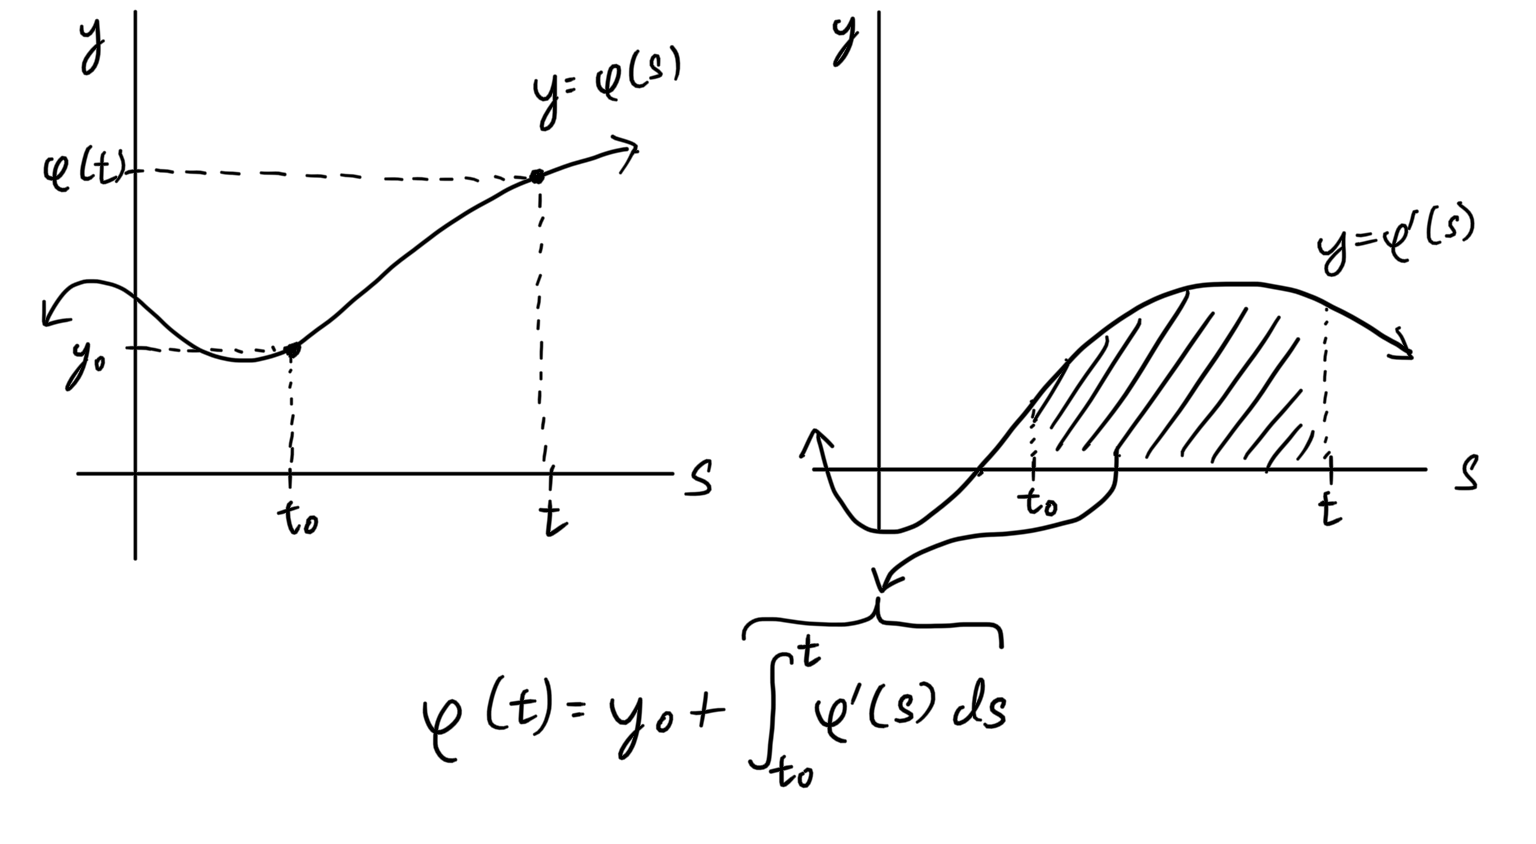
\includegraphics[scale=0.25]{img/Fundamental_Theorem_of_Calculus.PNG}
    \end{center}
    Since we know $y_0$, finding $f(t_0 + T)$ rests entirely on solving the integral representing the area under the velocity curve. Euler's method is simply doing this with left-hand Riemann sums. Note that while it is conventional that a the rectangles have the same width, they do not necessarily need to be. 
    \begin{enumerate}
        \item 2 Riemann rectangles (even and uneven). 
        \begin{center}
            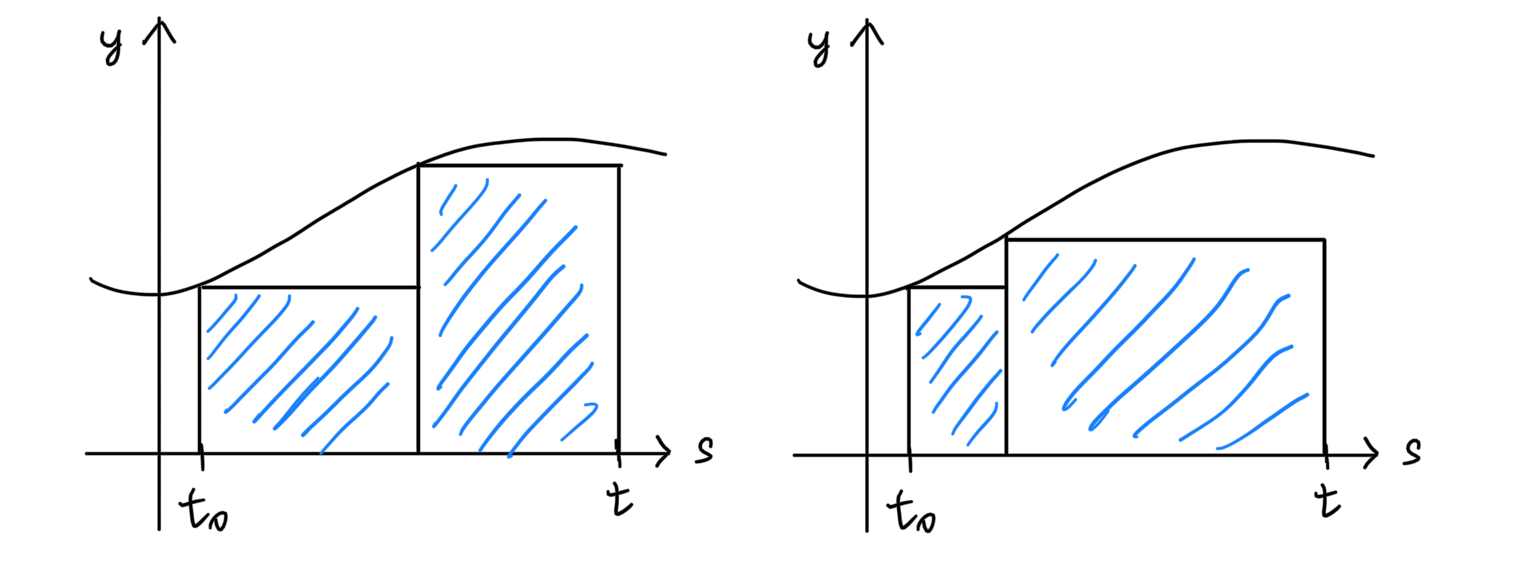
\includegraphics[scale=0.25]{img/2_Riemann.PNG}
        \end{center}
        \item 3 Riemann rectangles (even and uneven). 
        \begin{center}
            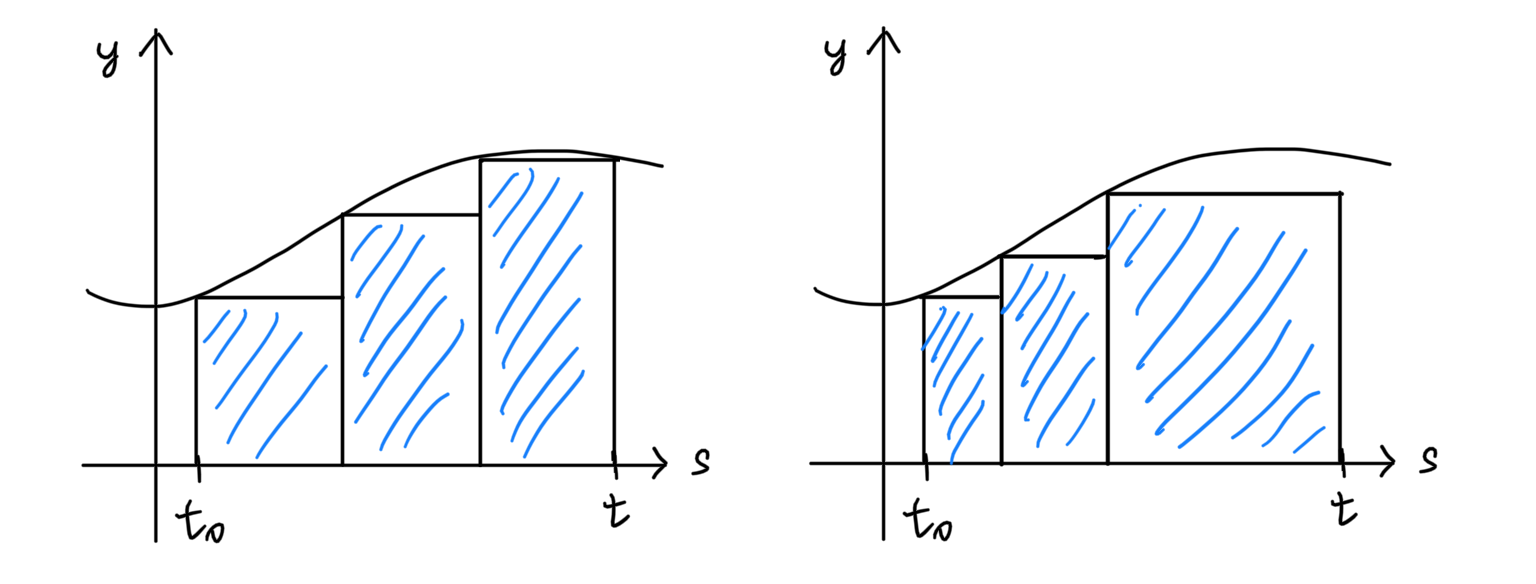
\includegraphics[scale=0.25]{img/3_Riemann.PNG}
        \end{center}
        \item 4 Riemann rectangles (even and uneven). 
        \begin{center}
            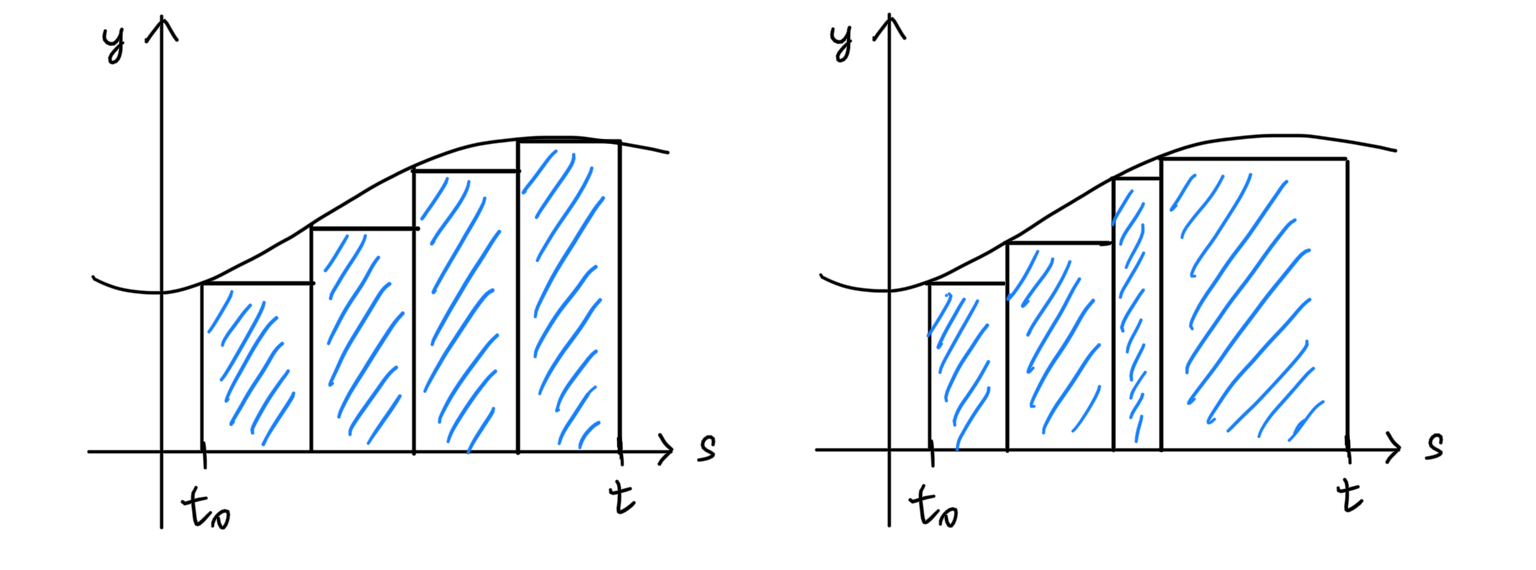
\includegraphics[scale=0.25]{img/4_Riemann.PNG}
        \end{center}
    \end{enumerate}
    In fact, the question of the best choice of unequal spacing is a major unsolved mathematical problem. We formalize this algorithm in the following steps. 

    \begin{theorem}[Euler's Method]
    Given the first order DEQ $y^\prime = f(t, y)$ with initial conditions $\varphi(t_0) = y_0$, say that we would like to approximate the value of $\varphi(t_0 + T)$. Then, the \textit{Euler method} gives us steps: 
    \begin{enumerate}
        \item Divide the interval $[t_0, t_0 + T]$ into $N$ (not necessarily equal) subintervals by specifying intermediate points
        \[t_0 < t_1 < t_2 < \ldots < t_{N-1} < t_N = t_0 + T\]
        For simplicity of calculations later, we will assume equal spacing, with spacing $h = T/N$. 
        \item Looking at points $t_k$ and $t_{k+1}$ for $k = 1, \ldots, N-1$, we can approximate the value of $y_{k+1}$ with $y_k$ using Riemann rectangles. 
        \begin{align*}
            y_{k+1} = y_k + \int_{t_k}^{t_{k+1}} f\big(s, \varphi(s)\big)\,ds  & \implies y_{k+1} = y_k + (t_{k+1} - t_k) f(t_k, y_k) \\
            & \implies y_{k+1} = y_k + h f(t_k, y_k)
        \end{align*}
        \begin{center}
            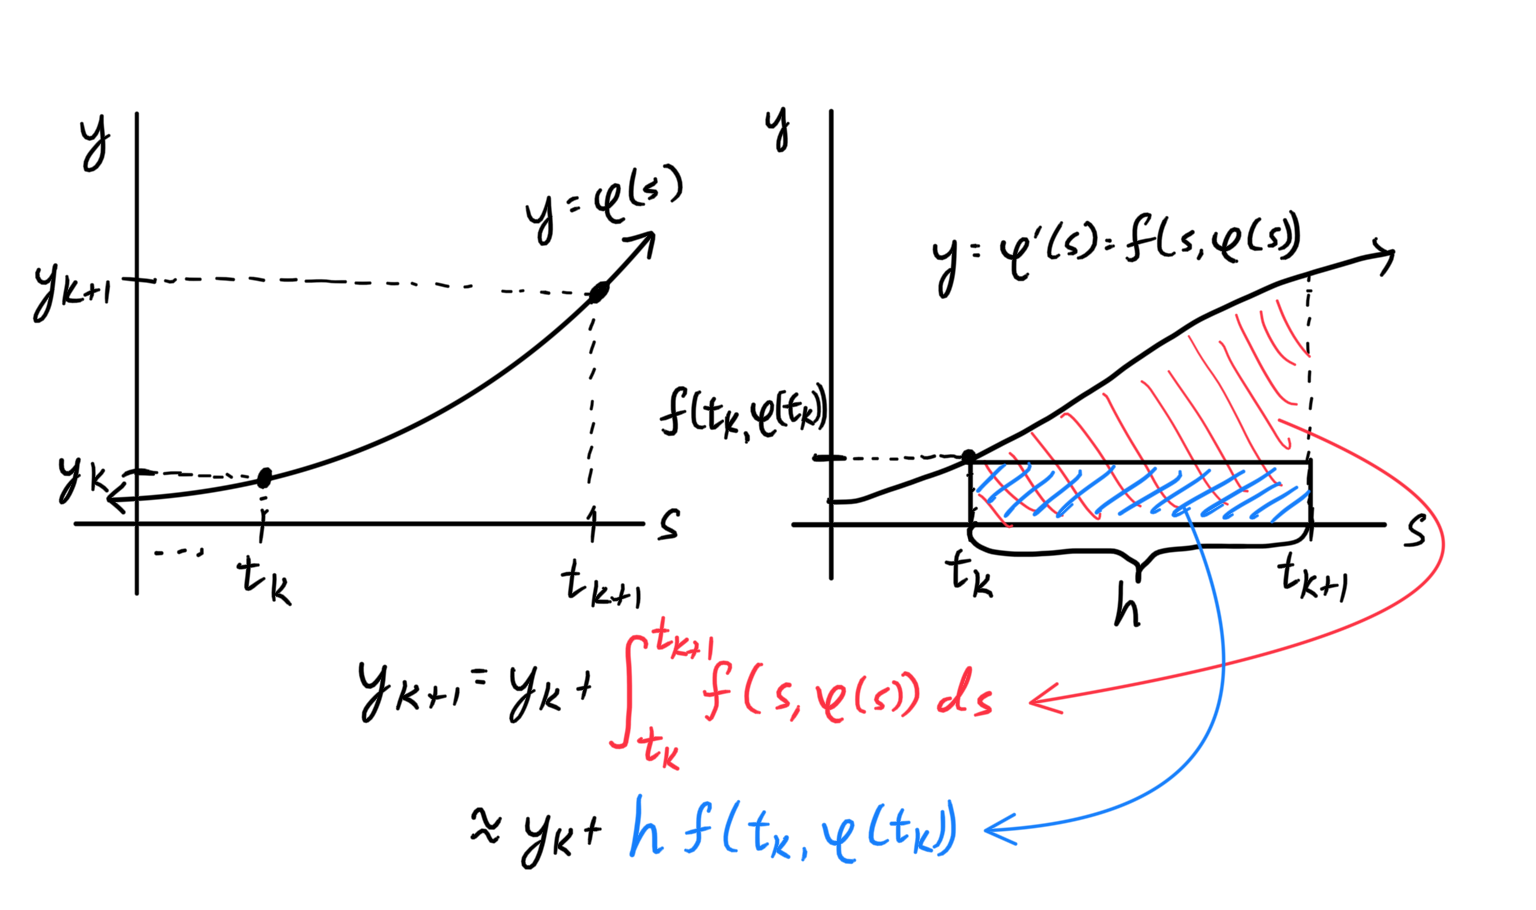
\includegraphics[scale=0.25]{img/Eulers_Method.PNG}
        \end{center}
        \item Use step 2 to find $y_1$, then $y_2$, and so on until $y_N \approx \varphi(t_N) = \varphi(t_0 + T)$ is found. Then terminate. 
    \end{enumerate}
    Furthermore, for some constant $M$, the local truncation error of the Euler method (for each step) is 
    \[|T_k| \leq \frac{1}{2} M h^2\]
    that is, no greater than a constant multiple of $h^2$, while the cumulative truncation error of it is
    \[|\varphi(t_n) - y_n| \leq \frac{1}{2} M h^2 N = \frac{1}{2} M T h\]
    that is, no greater than a constant multiple of $h$. 
    \end{theorem}

    Since the cumulative error bound is bounded by a linear function of $h$, we can make the error as small as we want by making the $h$ arbitrarily small. However, the truncation error for Euler's method is too large and is not used in applications. Rather, it is more efficient to use a more sophisticated method of approximation where the cumulative truncation error is no greater than a constant multiplied by some higher power of $h$. 

    An obvious improvement is to change the method of approximation of integrals from left-hand Riemann sums (taken at the start point of each interval) to Riemann rectangles taken at the midpoint of each interval. This method of approximation is called \textit{midpoint quadrature}
    \begin{center}
        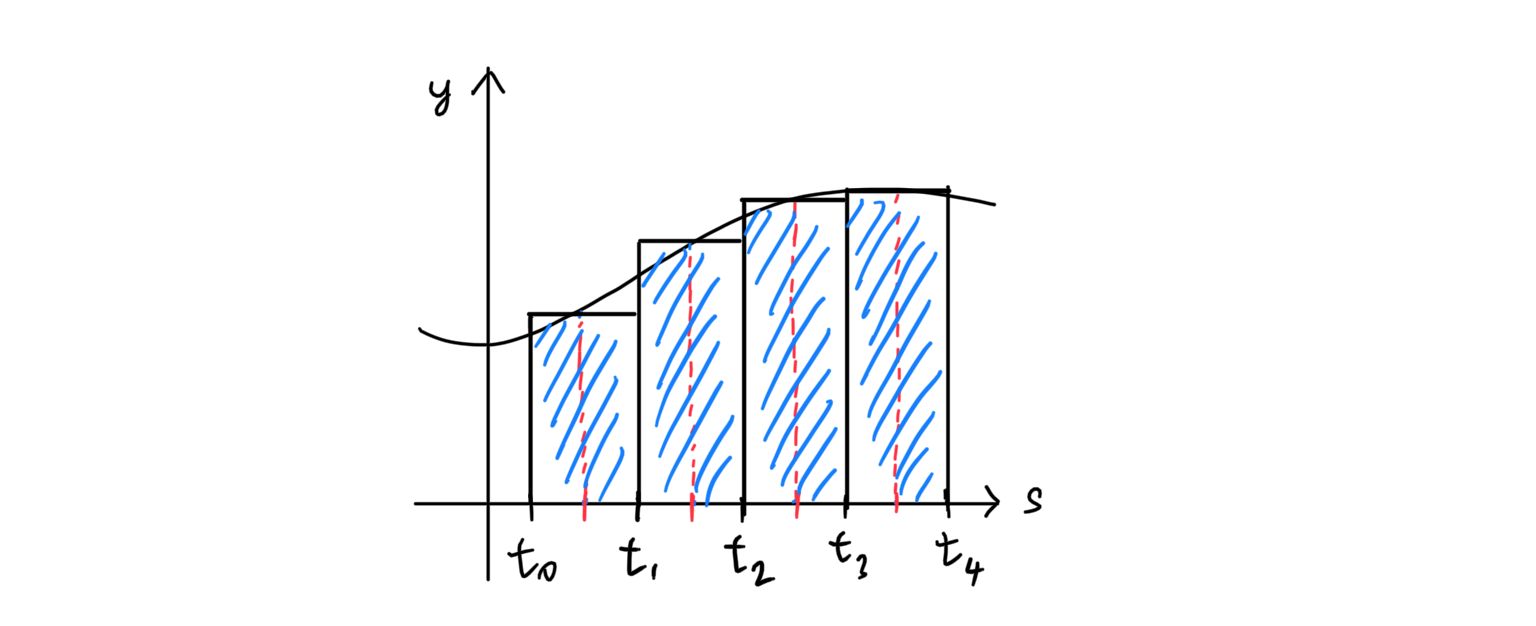
\includegraphics[scale=0.28]{img/Midpoint_Quadrature.PNG}
    \end{center}

    \begin{theorem}[Modified Euler's Method]
    Given the first order DEQ $y^\prime = f(t, y)$ with initial conditions $\varphi(t_0) = y_0$, say that we would like to approximate the value of $\varphi(t_0 + T)$.Then, the \textit{modified Euler's method} gives us steps: 
    \begin{enumerate}
        \item Divide the interval $[t_0, t_0 + T]$ into $N$ equal subintervals (of length $h$), where $N$ is an even number, by specifying intermediate points
        \[t_0 < t_1 < t_2 < \ldots < t_{N-1} < t_N = t_0 + T\]
        \item Rather than integrating over one subinterval $[t_k, t_{k+1}]$, we integrate over two subintervals $[t_k, t_{k+2}]$ and approximate it using the value of the function at $t_{k+1}$, the midpoint of the interval. That is, 
        \begin{align*}
            y_{k+2} = y_k + \int_{t_k}^{t_{k+2}} f\big(s, \varphi(s)\big)\,ds & \implies y_{k+2} = y_k + (t_{k+2} - t_k) f(t_{k+1}, y_{k+1}) \\
            & \implies y_{k+2} = y_k + 2 h f(t_{k+1}, y_{k+1})
        \end{align*}
        \begin{center}
            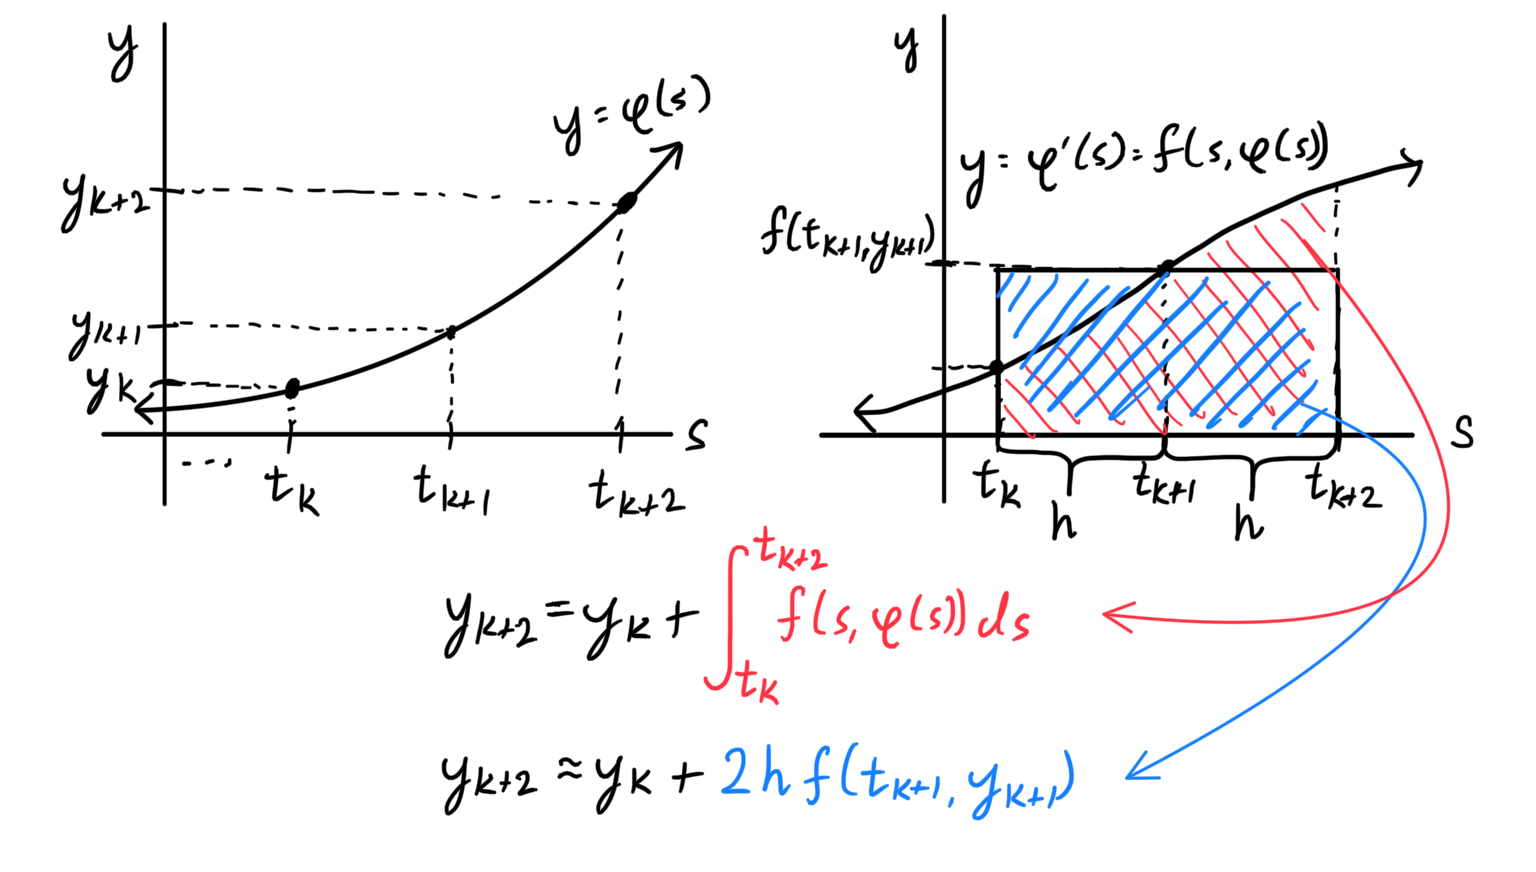
\includegraphics[scale=0.25]{img/Modified_Euler_Method.PNG}
        \end{center}
        Note that the modified Euler's method expresses $y_{k+2}$ in terms of both $y_k$ and $y_{k+1}$. This is a problem, since in the first step we know only $y_0$ but not $y_1$ in order to calculate $y_2$. Therefore, we must solve for $y_1$ with some other method, such as Euler's method or approximating using Taylor series (provided the function is analytic). 
        \item Use step to to find $y_2$, then $y_4$, then $y_6$, and so on until $y_N \approx \varphi(t_N) = \varphi(t_0 + T)$ is found. Then terminate. 
    \end{enumerate}
    Furthermore, for some constant $M$, the local truncation error of the modified Euler method (for each step) is 
    \[|T_k| \leq \frac{M}{3} h^3\]
    that is, no greater than a constant multiple of $h^2$, while the cumulative truncation error of it is no great than a constant multiple of $h^2$. 
    \end{theorem}

    \begin{example}[Comparison of Euler Algorithm and Modified Version on Approximating $e$]
    By setting $h = 0.1$, we estimate $e$ where $\varphi(1) = e$. Remember the differential equation with this solution is $y^\prime = f(t, y) = y$. Using Euler's method we have
    \[y_{k+1} = y_k + 0.1 y_k = 1.1y_k\]
    Doing this iteratively 10 times starting at $y_0 = 1$ gives us $1.1^{10} = 2.593$. However, using the modified Euler's method, we have 
    \[y_{k+2} = y_k + 0.2 f(t_{k+1}, y_{k+1})\]
    We can first approximate $y_1 = \varphi(0.1) = 1 + 0.1 + \frac{1}{2} (0.1)^2 + \ldots$ using a power series expansion, giving $y_1 \approx 1.105$ (correct to 3 decimal places). Since $f(t, y) = y$, we get 
    \[y_{k+2} = y_k + 0.2 y_{k+1}\]
    Calculating these values $y_2, y_3, \ldots$, we get $e \approx 2.713$, which is considerably better than the $2.593$ approximation. 
    \end{example}

    Another way to approximate definite integrals is to use trapezoidal sums as a method of approximation. 
    \[\int_{t_k}^{t_{k+1}} f\big(s, \varphi(s)\big)\,ds \approx \frac{h}{2}\big( f(t_k, \varphi(t_k)) + f(t_{k+1}, \varphi(t_{k+1}))\big)\]

    \begin{center}
        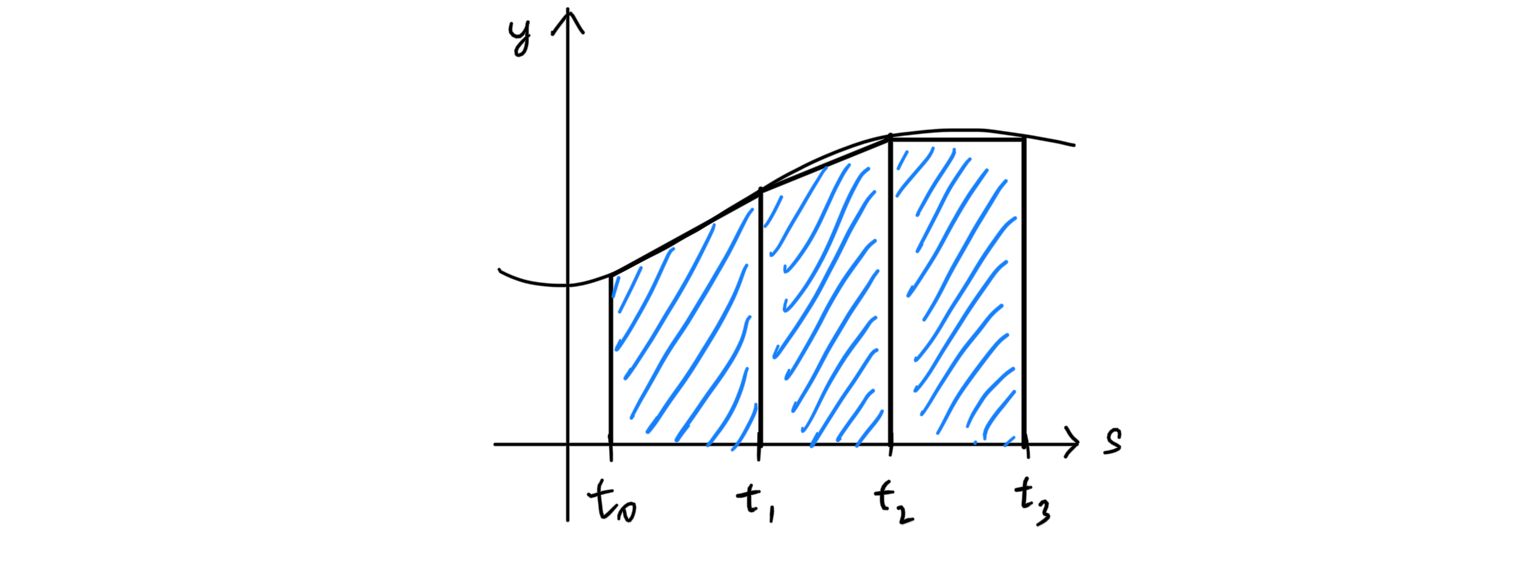
\includegraphics[scale=0.28]{img/Trapezoidal_Sum.PNG}
    \end{center}

    \begin{theorem}[Improved Euler's Method]
    Given the first order DEQ $y^\prime = f(t, y)$ with initial conditions $\varphi(t_0) = y_0$, say that we would like to approximate the value of $\varphi(t_0 + T)$, then the \textit{improved Euler method} gives us steps: 
    \begin{enumerate}
        \item Divide the interval $[t_0, t_0 + T]$ into $N$ (not necessarily equal) subintervals by specifying intermediate points 
        \[t_0 < t_1 < t_2 < \ldots < t_{N-1} < t_N = t_0 + T\]
        For simplicity of calculations later, we will assume equal spacing, with spacing $h = T/N$. 
        \item Looking at points $t_k$ and $t_{k+1}$ for $k = 1, \ldots, N-1$, we can approximate the value of $y_{k+1}$ with $y_k$ using trapezoids.
        \begin{align*}
            y_{k+1} = y_k + \int_{t_k}^{t_{k+1}} f\big( s, \varphi(s)\big)\,ds & \implies y_{k+1} = y_k + \frac{h}{2} \big(f(t_k, y_k) + f(t_{k+1}, y_{k+1}\big) 
        \end{align*}
        Note that the improved Euler method expresses $y_{k+1}$ implicitly rather than explicitly. There are methods for dealing with implicit formulas, but we leave it at this. 
        \item Use step 2 to find $y_2$, then $y_3$, and so on until $y_N \sum \varphi(t_N)$ is found. 
    \end{enumerate}
    \end{theorem}

  \subsection{The Milne Method}

    The Milne method gives us a quadratic approximation to certain integrals. 

    \begin{lemma}[Simpson's Rule]
    \textit{Simpson's rule} gives the approximation 
    \[\int_{t_k}^{t_{k+2}} f\big(s, \varphi(s)\big)\,ds \approx \frac{h}{3} \big( f(t_k, \varphi(t_k)) + 4 f (t_{k+1}, y_{k+1}) + f(t_{k+2}, y_{k+2})\big)\]
    \end{lemma}
    \begin{proof}
    This approximation pops up from attempting to find a quadratic graph of best fit for arbitrary function $y = f(t, \varphi(t))$. For convenience, we assign $F(t) = f(t, \varphi(t))$. Now, we must determine constants $a, b, c$ so that the parabola
    \[y = a + b(s - t_{k+1}) + c(s - t_{k+1})^2\]
    with vertex $(t_{k+1}, a)$ passes through the points $(t_k, F(t_k)), (t_{k+1}, F(t_{k+1})), (t_{k+2}, F(t_{k+2}))$. 
    \begin{center}
        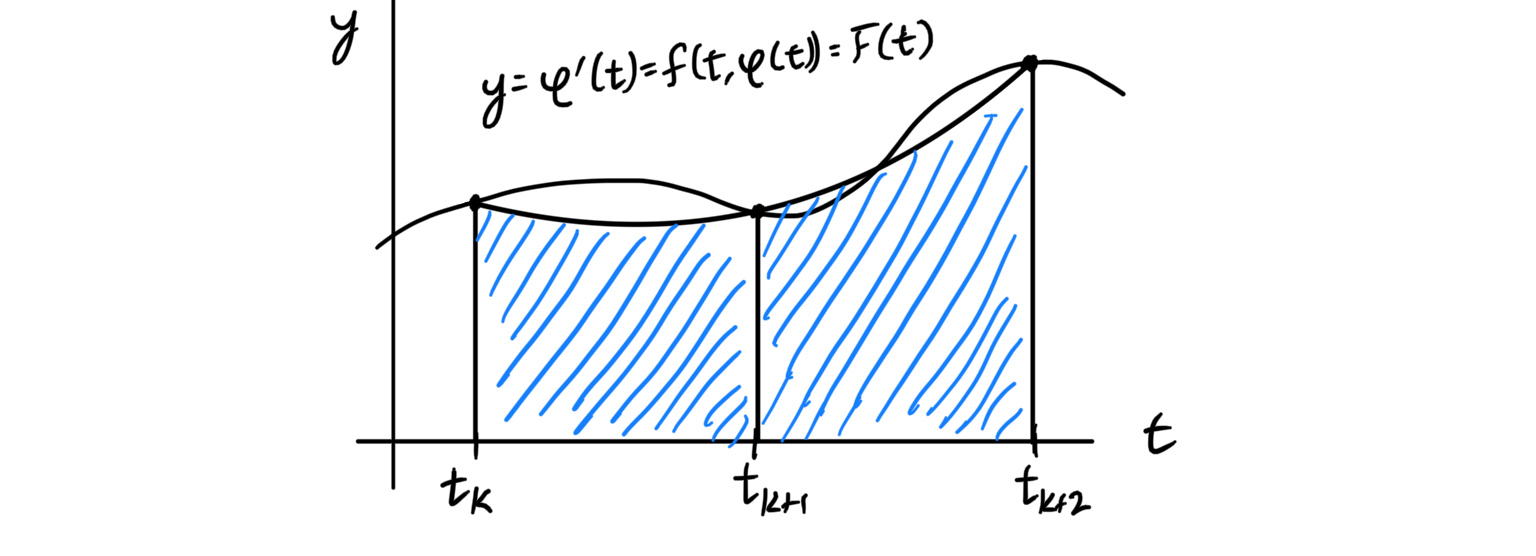
\includegraphics[scale=0.27]{img/Quadratic_Milne.PNG}
    \end{center}
    Since $h = t_{k+2} - t_{k+1} = t_{k+1} - t_k$, we have the set of conditions
    \begin{align*}
        F(t_k) & = a - bh + ch^2 \\
        F(t_{k+1}) & = a \\
        F(t_{k+2}) & = a + bh + ch^2
    \end{align*}
    We can solve this system to get
    \[a = F(t_{k+1}), \;\;\;\;\; c = \frac{F(t_{k+2}) - 2 F (t_{k+1}) + F(t_k)}{2 h^2}\]
    We then integrate this quadratic approximation
    \begin{align*}
        \int_{t_k}^{t_{k+2}} \big( a + b(s - t_{k+1}) + c(s - t_{k+1})^2 \big) \,ds & = \bigg( as - \frac{b}{2} (s - t_{k+1})^2 + \frac{c}{3} (s - t_{k+1})^3 \bigg) \bigg|^{t_{k+2}}_{t_k} \\
        & = 2 ah + \frac{2}{3} ch^3
    \end{align*}
    Note that we do not even need to find the value of $b$. Substituting the solutions $a, c$ in, we get Simpson's Rule. 
    \end{proof}

    \begin{theorem}[Milne Method]
    Given the first order DEQ $y^\prime = f(t, y)$ with initial conditions $\varphi(t_0) = y_0$, say that we would like to approximate the value of $\varphi(t_0 + T)$. Then, the \textit{Milne method} gives us steps: 
    \begin{enumerate}
        \item Divide the interval $[t_0, t_0 + T]$ into $N$ (not necessarily equal) subintervals by specifying intermediate points 
        \[t_0 < t_1 < t_2 < \ldots < t_{N-1} < t_N = t_0 + T\]
        For simplicity of calculations later, we will assume equal spacing, with spacing $h = T/N$. 
        \item Rather than integrating over one subinterval $[t_k, t_{k+1}]$, we integrate over two subintervals $[t_k, t_{k+2}]$ and approximate it using Milne's formula:
        \begin{align*}
            y_{k+2} = y_k & + \int_{t_k}^{t_{k+2}} f\big(s, \varphi(s)\big)\,ds \\
            \implies & y_{k+2} = y_k + \frac{h}{3} \big( f(t_k, \varphi(t_k)) + 4 f (t_{k+1}, y_{k+1}) + f(t_{k+2}, y_{k+2})\big)
        \end{align*}
        Note that this solves for $y_{k+2}$ implicitly (which isn't a problem when dealing with linear equations), and you need to know both $y_k$ and $y_{k+1}$ in order to calculate $y_{k+2}$. 
        \item Use step 2 to find $y_2, y_3, \ldots$ until $y_N \approx \varphi(t_N)$ is found. Then terminate. 
    \end{enumerate}
    Furthermore, the cumulative truncation error of the Milne method is no greater than a constant multiple of $h^4$. 
    \end{theorem}

    We can now state a very important theorem on error bounds of one-step methods (applying to the Euler method, but not to the Milne method). 

    \begin{theorem}[Truncation Error Bounds on One-Step Methods]
    Suppose that $f(t, y) \in C^1$ for $t_0 \leq t \leq t_0 + T$ and all $y$. Suppose 
    \[y_1, y_2, \ldots, y_N\]
    are the approximations calculated by some one-step method with step length $h$ to the solution $\varphi$ of 
    \[y^\prime = f(t, y), \;\;\;\; \varphi(t_0) = y_0\]
    If the local truncation error is no greater than $\epsilon$, then the cumulative truncation error is no greater than a constant multiple of $\epsilon/h$. 
    \end{theorem}

    This theorem shows that if the local truncation error of a one-step process is no greater than a constant multiple of $h^p$, then the cumulative truncation error is no grater than a constant multiple of $h^{p-1}$. Analogous results can be proved for two-steps methods (and for methods involving any finite number of steps). Therefore, the accuracy of approximation is improved if a method whose truncation error involves a higher power of $h$ is used. 

  \subsection{Stability, Consistency, and Convergence}

    \begin{definition}[Round-Off Errors]
    When we use a numerical method to obtain an approximation to the solution of a differential equation, we are trying to find a set of numbers 
    \[y_1, y_2, y_3, \ldots, y_N\]
    defined by the method, where $y_N$ is the final approximation. However, due to the floating-point nature of numbers in computers, we actually round-off all numbers calculated to a specific number of significant figures, obtaining a slightly different set of numbers
    \[z_1, z_2, z_3, \ldots, z_N\]
    the difference
    \[r_k = |z_k - y_k|, \;\; k = 1, 2, \ldots, N\]
    is called the \textit{round-off error}. The $h$ value is also called the \textit{mesh}. 
    \end{definition}

    \begin{definition}[Finite-Difference Methods]
    \textit{Finite-difference} methods are a class of numerical techniques for solving differential equations by approximating derivatives with finite differences. Both the spatial domain and time interval are discretized (i.e. broken up into a finite number of steps), and the value of the solution at these discrete points is approximated by solving algebraic equations containing finite differences and values from nearby points. 
    \end{definition}

    \begin{definition}[Consistency, Stability, Convergence]
    We now define three common terms that describes numerical methods. 
    \begin{enumerate}
        \item \textit{Consistency}: A finite difference method is considered consistent if by reducing the mesh and time step size, the truncation error terms could be made to approach $0$. In this case the solution to the difference equation would approach the true solution of the DE. 
        \item \textit{Stability}: A finite difference approximation is stable if the errors (truncation, round-off, etc.) decay (i.e. remain bounded, preferably within some deducible function) as the computation proceeds from one marching step to the next. 
        \item \textit{Convergence}: The solution to the finite difference approximation approaches the true solution of the DE when the mesh is refined (step size reduced). This means that the approximation $y_N$ tend to the actual solution as $h \rightarrow 0$. 
    \end{enumerate}
    \end{definition}

    Every method mentioned in this section is convergent. Obviously, a method which is not convergent is useless for obtaining numerical approximations. It is possible to give conditions for stability and consistency of numerical methods which are easy to verify. If we do this, we can use the following theorem to prove convergence. 

    \begin{theorem}[Lax Equivalence Theorem]
    A finite difference approximation method satisfying consistency (meaning truncation error approaches $0$ when step size and mesh size goes to $0$) and stability (meaning error goes on diminishing as time step passes) is convergent. 
    \end{theorem}

    It turns out that the Milne method may be numerically instable, which is why it is not always suitable, despite its small truncation error. 

  \subsection{Runge-Kutta Methods}

    Let us revisit Taylor polynomials that serve as approximations to differentiable functions. Let $\varphi$ be the solution of the differential equation 
    \[y^\prime = f(t, y) , \;\;\;\; \varphi(t_0) = y_0\]
    Assuming that $\varphi$ has a continuous second derivative on the interval $[t_0, t_0 + T]$, we can use Taylor's theorem (with the Lagrange form of the remainder) to write the first order approximation centered at $t_0$.  
    \[\varphi(t) = \varphi(t_0) + (t - t_0) \varphi^\prime (t_0) + \frac{(t - t_0)^2}{2!} \varphi^{\prime\prime} (\zeta)\]
    for some $\zeta \in (t_0, t)$. If $t_1 = t_0 + h$, then
    \begin{align*}
        \varphi(t_1) & = \varphi(t_0) + h \varphi^\prime (t_0) + \frac{h^2}{2!} \varphi^{\prime\prime} (\zeta) \\
        & = \varphi(t_0) + h f(t_0, y_0) + \frac{h^2}{2!} \varphi^{\prime\prime} (\zeta) \\
        & \approx y_0 + h f(t_0, y_0)
    \end{align*}
    where the approximation is gotten by neglecting the term $\frac{h^2}{2!} \varphi^{\prime\prime} (\zeta)$. If we divide the interval $[t_0, t_0 + T]$ into $N$ subintervals of length $h$ by defining the partition points $t_k = t_0 + kh$ ($k = 0, 1, \ldots, N$), we can use this procedure to obtain an iterative formula
    \[y_{k+1} = y_k + hf(t_k, y_k)\]
    with local truncation error $\frac{h^2}{2!} \varphi^{\prime\prime} (\zeta)$. This first-order approximation is, of course, just Euler's algorithm. 

    If we look at the second degree Taylor expansion 
    \[\varphi(t) = \varphi(t_0) + (t - t_0) \varphi^\prime (t_0) + \frac{(t - t_0)^2}{2!} \varphi^{\prime\prime} (t_0) + \frac{(t - t_0)^3}{3!} \varphi^{\prime\prime\prime} (\zeta)\]
    we can ignore the error term but we still have to deal with the second order term. We can evaluate $\varphi^{\prime\prime} (t_0)$ by differentiating $\varphi^\prime (t) = f(t, \varphi(t))$ using the chain rule, which gives
    \begin{align*}
        \varphi^{\prime\prime} (t) & = f_t \big( t, \varphi(t)\big) + f_y \big(t, \varphi(t)\big) \varphi^\prime (t) \\
        & = f_t \big(t, \varphi(t)\big) + f_y \big( t, \varphi(t)\big) f\big(t, \varphi(t)\big)
    \end{align*}
    Where $f_t$ and $f_y$ represents the partial derivatives with respect to $t$ and $y$, respectively. Note that when computing $f_t (t, \varphi(t))$, we should keep $\varphi(t)$ constant, and when computing $f_y (t, \varphi(t))$, we should keep $t$ constant while deriving with respect to $y = \varphi(t)$. Do not get confused by this. This ultimately leads to the iterative approximation formula
    \[y_{k+1} = y_k + h f(t_k, y_k) + \frac{h^2}{2!} \big( f_t (t_k, y_k) + f_y (t_k, y_k) f(t_k, y_k)\big)\]
    with local truncation error $\frac{h^3}{3!} \varphi^{\prime\prime\prime} (\zeta)$. This is a plausible means of obtaining numerical approximations, but it suffers from the disadvantage of having to calculate derivatives of $f$, which isn't easy for a computer to do. This problem persists for procedures using higher-order Taylor approximations. 

    The Runge-Kutta method is an attempt to obtain formulas equivalent to Taylor approximations which do not involve derivatives of $f$. There are many variations of Runge-Kutta methods, but we will describe the most common version. 

    \begin{theorem}[Runge-Kutta Method]
    Given the first order DEQ $y^\prime = f(t, y)$ with initial conditions $\varphi(t_0) = y_0$, say that we would like to approximate the value of $\varphi(t_0 + T)$. Then, the \textit{Runge-Kutta method} gives us steps: 
    \begin{enumerate}
        \item Divide the interval $[t_0, t_0 + T]$ into $N$ (not necessarily equal) subintervals by specifying intermediate points 
        \[t_0 < t_1 < t_2 < \ldots < t_{N-1} < t_N = t_0 + T\]
        For simplicity of calculations later, we will assume equal spacing, with spacing $h = T/N$. 
        \item Given the value $y_k$, we can approximate the value $y_{k+1}$ using the one-step process
        \[y_{k+1} = y_k + \frac{h}{6} (p_1 + 2p_2 + 2p_3 + p_4)\]
        where 
        \begin{align*}
            p_1 & = f(t_k, y_k) & & p_2 = f\bigg( t_k + \frac{h}{2}, y_k + \frac{h p_1}{2}\bigg)  \\
            p_3 & = f\bigg( t_k + \frac{h}{2} , y_k + \frac{h p_2}{2} \bigg) & & p_4 = f(t_{k+1}, y_k + h p_3)
        \end{align*}
    \end{enumerate}
    The term $\frac{1}{6} (p_1 + 2p_2 + 2p_3 + p_4)$ represents an "average" slope of $\varphi$ over the interval $[t_k, t_{k+1}]$. More specifically, 
    \begin{enumerate}
        \item $p_1$ is the slope at $t_1$
        \item $p_2$ is an approximation of the slops at the midpoint of the interval obtained by means of the Euler method
        \item $p_3$ is a second approximation to the slope at the midpoint
        \item $p_4$ is an approximation to the slope at $t_{k+1}$ obtained by means of the Euler method with slope $p_3$. 
    \end{enumerate}
    Even though it requires a lot of calculations, it is an explicit one-step procedure that does not require calculation of derivative of $f$. Furthermore, it is equivalent to a 4th order Taylor formula, and the local truncation error of the Runge-Kutta method is no greater than a constant multiple of $h^5$. 
    \end{theorem}

    \begin{example}[Deriving a Runge-Kutta Formula equivalent to 2nd-Order Taylor Formula]
    Earlier in this subsection, we have found that the second order approximation formula for $\varphi$ is 
    \[y_{k+1} = y_k + h f(t_k, y_k) + \frac{h^2}{2!} \big( f_t (t_k, y_k) + f_y (t_k, y_k) f(t_k, y_k)\big)\]
    which requires us to compute derivatives. We will demonstrate how to obtain a Runge-Kutta formula equivalent to this 2nd-order Taylor formula. We will assume a method of form 
    \[y_{k+1} = y_k + h \Big( af(t_k, y_k) + b f\big( t_k + \alpha h, y_k + \beta h f(t_k, t_k)\big)\Big)\]
    where $a, b, \alpha, \beta$ are constants to be determined. By Taylor's theorem for functions of two variables we write
    \[f\big(t_k + \alpha h, y_k + \beta h f(t_k, y_k)\big) = f(t_k, y_k) + \alpha h f_t (t_k, y_k) + \beta h f(t_k, y_k) f_y (t_k, y_k) + R h^2\]
    where $R$ is a remainder term involving the second-order partial derivatives of $f$. Substituting this into the original form gives
    \begin{align*}
        y_{k+1} = y_k + h(a + b) f(t_k, y_k) + h^2 \big( \alpha b f_t (t_k, y_k) + \beta b f(t_k, y_k) f_y (t_k, y_k)\big) + R b h^3
    \end{align*}
    Comparing this with the original approximation formula for $\varphi$ (with derivatives), we can compare each term and see that if
    \[a + b = 1, \;\;\;, \alpha b = \frac{1}{2}, \;\;\; \beta b = \frac{1}{2}\]
    then the approximations obtained by these two formulas differ only by the term $R b h^3$. Thus, any quadruples of constants satisfying these conditions is a Runge-Kutta formula of the desired type. For example, choosing $a = \frac{1}{2}, b = \frac{1}{2}, \alpha = 1, \beta = 1$, gives
    \[y_{k+1} = y_k + \frac{h}{2} \big( f(t_k, y_k) + f(t_{k+1}, y_k + h f(t_k, y_k))\big)\]
    which is equivalent in accuracy to a three-term Taylor formula. Also note that this formula is similar to the improved Euler method. 
    \end{example}

  \subsection{Numerical Methods for Systems and Equations of Higher Order}

    Everything in this section had been designed for first-order equations, but these methods are equally suitable for systems of differential equations. We can write a system of equations as a vector equation
    \[y^\prime = f(t, y) \iff \begin{cases}
    y_1^\prime & = f_1 (t, y_1, y_2, \ldots, y_n) \\
    y_2^\prime & = f_2 (t, y_1, y_2, \ldots, y_n) \\
    \vdots & = \vdots \\
    y_n^\prime & = f_n (t, y_1, y_2, \ldots, y_n)
    \end{cases}\]
    where $y \in \mathbb{R}^n$ and $f: \mathbb{R}^n \times \mathbb{R} \longrightarrow \mathbb{R}^n$. We can apply the approximation methods developed in this chapter to the system by applying them to each component in the vector equation. 

    \begin{example}
    Consider the system 
    \[u^\prime = v, \;\;\;\; v^\prime = g(t, u, v)\]
    This can be written in form 
    \[y^\prime = f(t, y) \iff \begin{pmatrix} u \\ v \end{pmatrix}^\prime = \begin{pmatrix} v \\ g(t, u, v) \end{pmatrix} \]
    The Euler method applied to this system leads to a pair of iterative formulas 
    \[\begin{pmatrix} u_{k+1} \\ v_{k+1} \end{pmatrix} = \begin{pmatrix} u_k \\ v_k \end{pmatrix} + h \begin{pmatrix} v_k \\ g(t_k, u_k, v_k) \end{pmatrix} \implies \begin{cases} u_{k+1} & = u_k + h v_k \\
    v_{k+1} & = v_k + h g(t_k, u_k, v_k) \end{cases}\]
    Therefore, once we are given initial values $u_0$ and $v_0$, and once we have found both $u_k$ and $v_k$, we can use this to compute $u_{k+1}$ and $v_{k+1}$. 
    \end{example}

    As we have seen before, higher order equations can be treated as a system of first-order DEQs, which can then be solved numerically on each component equation. 

\end{document}

